\documentclass[8pt,aspectratio=1610]{beamer}
\usepackage[utf8]{inputenc}
\usepackage{booktabs}
\usepackage{array}
\usepackage{graphicx}
\usepackage{xcolor}
\usepackage{tikz}
\usetikzlibrary{positioning,arrows.meta,decorations.pathreplacing,calc,shadows}
\usepackage{pgfplots}
\pgfplotsset{compat=1.18}
\usepackage{amsmath}
\usepackage{amssymb}
\usepackage{amsfonts}
\usepackage{algorithm}
\usepackage{algorithmic}

\usetheme{metropolis}
\usecolortheme{wolverine}
\metroset{progressbar=frametitle,block=fill}
\setbeamertemplate{navigation symbols}{}

% Define custom colors complementing the Wolverine theme
\definecolor{maizelight}{RGB}{255, 203, 5}
\definecolor{maizedark}{RGB}{255, 167, 0}
\definecolor{bluelight}{RGB}{0, 39, 76}
\definecolor{tealaccent}{RGB}{0, 128, 128}
\definecolor{orangeaccent}{RGB}{255, 138, 51}

% Customize block colors
\setbeamercolor{block title}{bg=bluelight,fg=white}
\setbeamercolor{block body}{bg=bluelight!10,fg=black}
\setbeamercolor{block title example}{bg=maizelight,fg=black}
\setbeamercolor{block body example}{bg=maizelight!15,fg=black}
\setbeamercolor{block title alerted}{bg=orangeaccent,fg=white}
\setbeamercolor{block body alerted}{bg=orangeaccent!15,fg=black}

% Custom block environments
\newenvironment<>{techblock}[1]{%
  \setbeamercolor{block title}{bg=tealaccent,fg=white}%
  \setbeamercolor{block body}{bg=tealaccent!10,fg=black}%
  \begin{block}#2{#1}}{\end{block}}

\newenvironment<>{tipblock}[1]{%
  \setbeamercolor{block title}{bg=maizedark,fg=black}%
  \setbeamercolor{block body}{bg=maizedark!15,fg=black}%
  \begin{block}#2{#1}}{\end{block}}

% Title slide information
\title{Classification Methods}
\subtitle{CMSC 173 - Machine Learning}
\author{Noel Jeffrey Pinton}
\institute{Department of Computer Science\\University of the Philippines - Cebu}
\date{\today}

\begin{document}

\begin{frame}
\titlepage
\end{frame}

\begin{frame}{Outline}
\tableofcontents
\end{frame}

% ========================================
% Section: Introduction
% ========================================

\section{Introduction \& Motivation}

\begin{frame}{What is Classification?}
\begin{columns}[t]
\begin{column}{0.48\textwidth}
\begin{block}{Definition}
\textbf{Classification} is a supervised learning task where we predict a discrete class label for new observations based on training examples.
\end{block}

\vspace{0.2cm}

\begin{exampleblock}{Key Characteristics}
\begin{itemize}
\setlength{\itemsep}{2pt}
\item Supervised learning
\item Discrete output (classes/categories)
\item Learn from labeled training data
\item Make predictions on new data
\end{itemize}
\end{exampleblock}
\end{column}

\begin{column}{0.48\textwidth}
\begin{block}{Formulation}
Given training data:
$$\mathcal{D} = \{(\mathbf{x}_1, y_1), \ldots, (\mathbf{x}_n, y_n)\}$$

where:
\begin{itemize}
\setlength{\itemsep}{1pt}
\item $\mathbf{x}_i \in \mathbb{R}^d$ = feature vector
\item $y_i \in \{1, 2, \ldots, C\}$ = class label
\end{itemize}

\vspace{0.1cm}

\textbf{Goal:} Learn function $f: \mathbb{R}^d \rightarrow \{1, \ldots, C\}$
\end{block}

\vspace{0.1cm}

\begin{alertblock}{Types}
\textbf{Binary:} 2 classes (spam/not spam)\\
\textbf{Multi-class:} $C > 2$ classes (digits 0-9)
\end{alertblock}
\end{column}
\end{columns}
\end{frame}

\begin{frame}{Classification vs Regression}
\begin{columns}[t]
\begin{column}{0.48\textwidth}
\begin{block}{Classification}
\begin{itemize}
\setlength{\itemsep}{2pt}
\item \textbf{Output:} Discrete categories
\item \textbf{Examples:}
  \begin{itemize}
  \setlength{\itemsep}{0pt}
  \item Email: spam/not spam
  \item Medical: disease diagnosis
  \item Image: object recognition
  \item Finance: loan approval
  \end{itemize}
\item \textbf{Metrics:} Accuracy, precision, recall
\item \textbf{Goal:} Predict class membership
\end{itemize}
\end{block}
\end{column}

\begin{column}{0.48\textwidth}
\begin{block}{Regression}
\begin{itemize}
\setlength{\itemsep}{2pt}
\item \textbf{Output:} Continuous values
\item \textbf{Examples:}
  \begin{itemize}
  \setlength{\itemsep}{0pt}
  \item House price prediction
  \item Temperature forecasting
  \item Stock price estimation
  \item Age prediction
  \end{itemize}
\item \textbf{Metrics:} MSE, MAE, $R^2$
\item \textbf{Goal:} Predict numerical value
\end{itemize}
\end{block}
\end{column}
\end{columns}

\vspace{0.1cm}

\begin{alertblock}{Key Difference}
Classification predicts \textbf{categories}, regression predicts \textbf{quantities}.
\end{alertblock}
\end{frame}

\begin{frame}{Real-World Applications}
\begin{columns}[t]
\begin{column}{0.48\textwidth}
\begin{block}{Medical \& Healthcare}
\begin{itemize}
\setlength{\itemsep}{2pt}
\item \textbf{Disease diagnosis}: Cancer detection, diabetes screening
\item \textbf{Medical imaging}: X-ray, MRI classification
\item \textbf{Drug discovery}: Molecular classification
\end{itemize}
\end{block}

\vspace{0.15cm}

\begin{block}{Finance \& Business}
\begin{itemize}
\setlength{\itemsep}{2pt}
\item \textbf{Credit scoring}: Loan default prediction
\item \textbf{Fraud detection}: Transaction classification
\item \textbf{Customer churn}: Retention analysis
\end{itemize}
\end{block}
\end{column}

\begin{column}{0.48\textwidth}
\begin{block}{Technology \& Media}
\begin{itemize}
\setlength{\itemsep}{2pt}
\item \textbf{Image recognition}: Object detection, face recognition
\item \textbf{Text classification}: Sentiment analysis, spam filtering
\item \textbf{Recommendation}: Content categorization
\end{itemize}
\end{block}

\vspace{0.15cm}

\begin{block}{Science \& Engineering}
\begin{itemize}
\setlength{\itemsep}{2pt}
\item \textbf{Biology}: Species identification, gene classification
\item \textbf{Quality control}: Defect detection
\item \textbf{Remote sensing}: Land cover classification
\end{itemize}
\end{block}
\end{column}
\end{columns}

\vspace{0.05cm}

\begin{alertblock}{Common Theme}
All involve learning patterns from labeled examples to classify new instances!
\end{alertblock}
\end{frame}

\begin{frame}{Classification Methods Overview}
\textbf{This lecture covers three fundamental classification methods:}

\vspace{0.3cm}

\begin{columns}[t]
\begin{column}{0.32\textwidth}
\begin{block}{Naive Bayes}
\textbf{Probabilistic}
\begin{itemize}
\setlength{\itemsep}{1pt}
\item Based on Bayes theorem
\item Assumes feature independence
\item Fast, simple
\item Works with small data
\end{itemize}

\vspace{0.05cm}

\textbf{Best for:} Text classification, real-time prediction
\end{block}
\end{column}

\begin{column}{0.32\textwidth}
\begin{block}{K-Nearest Neighbors}
\textbf{Instance-based}
\begin{itemize}
\setlength{\itemsep}{1pt}
\item Distance-based
\item Non-parametric
\item No training phase
\item Intuitive
\end{itemize}

\vspace{0.05cm}

\textbf{Best for:} Pattern recognition, recommendation systems
\end{block}
\end{column}

\begin{column}{0.32\textwidth}
\begin{block}{Decision Trees}
\textbf{Rule-based}
\begin{itemize}
\setlength{\itemsep}{1pt}
\item Hierarchical decisions
\item Interpretable
\item Handles mixed types
\item Foundation for ensembles
\end{itemize}

\vspace{0.05cm}

\textbf{Best for:} Medical diagnosis, credit scoring
\end{block}
\end{column}
\end{columns}

\vspace{0.2cm}

\begin{alertblock}{Learning Objectives}
Understand theory, implementation, and practical application of each method.
\end{alertblock}
\end{frame}

% ========================================
% Section: Naive Bayes
% ========================================

\section{Naive Bayes Classification}

\begin{frame}{Bayes' Theorem: Foundation}

\begin{block}{Bayes' Theorem}
$$P(C_k | \mathbf{x}) = \frac{P(\mathbf{x} | C_k) \cdot P(C_k)}{P(\mathbf{x})}$$

where:
\begin{itemize}
\setlength{\itemsep}{1pt}
\item $P(C_k | \mathbf{x})$ = \textbf{Posterior}: Probability of class $C_k$ given features $\mathbf{x}$
\item $P(\mathbf{x} | C_k)$ = \textbf{Likelihood}: Probability of features given class
\item $P(C_k)$ = \textbf{Prior}: Probability of class (before seeing data)
\item $P(\mathbf{x})$ = \textbf{Evidence}: Probability of features (normalization constant)
\end{itemize}
\end{block}

\vspace{0.15cm}

\centering
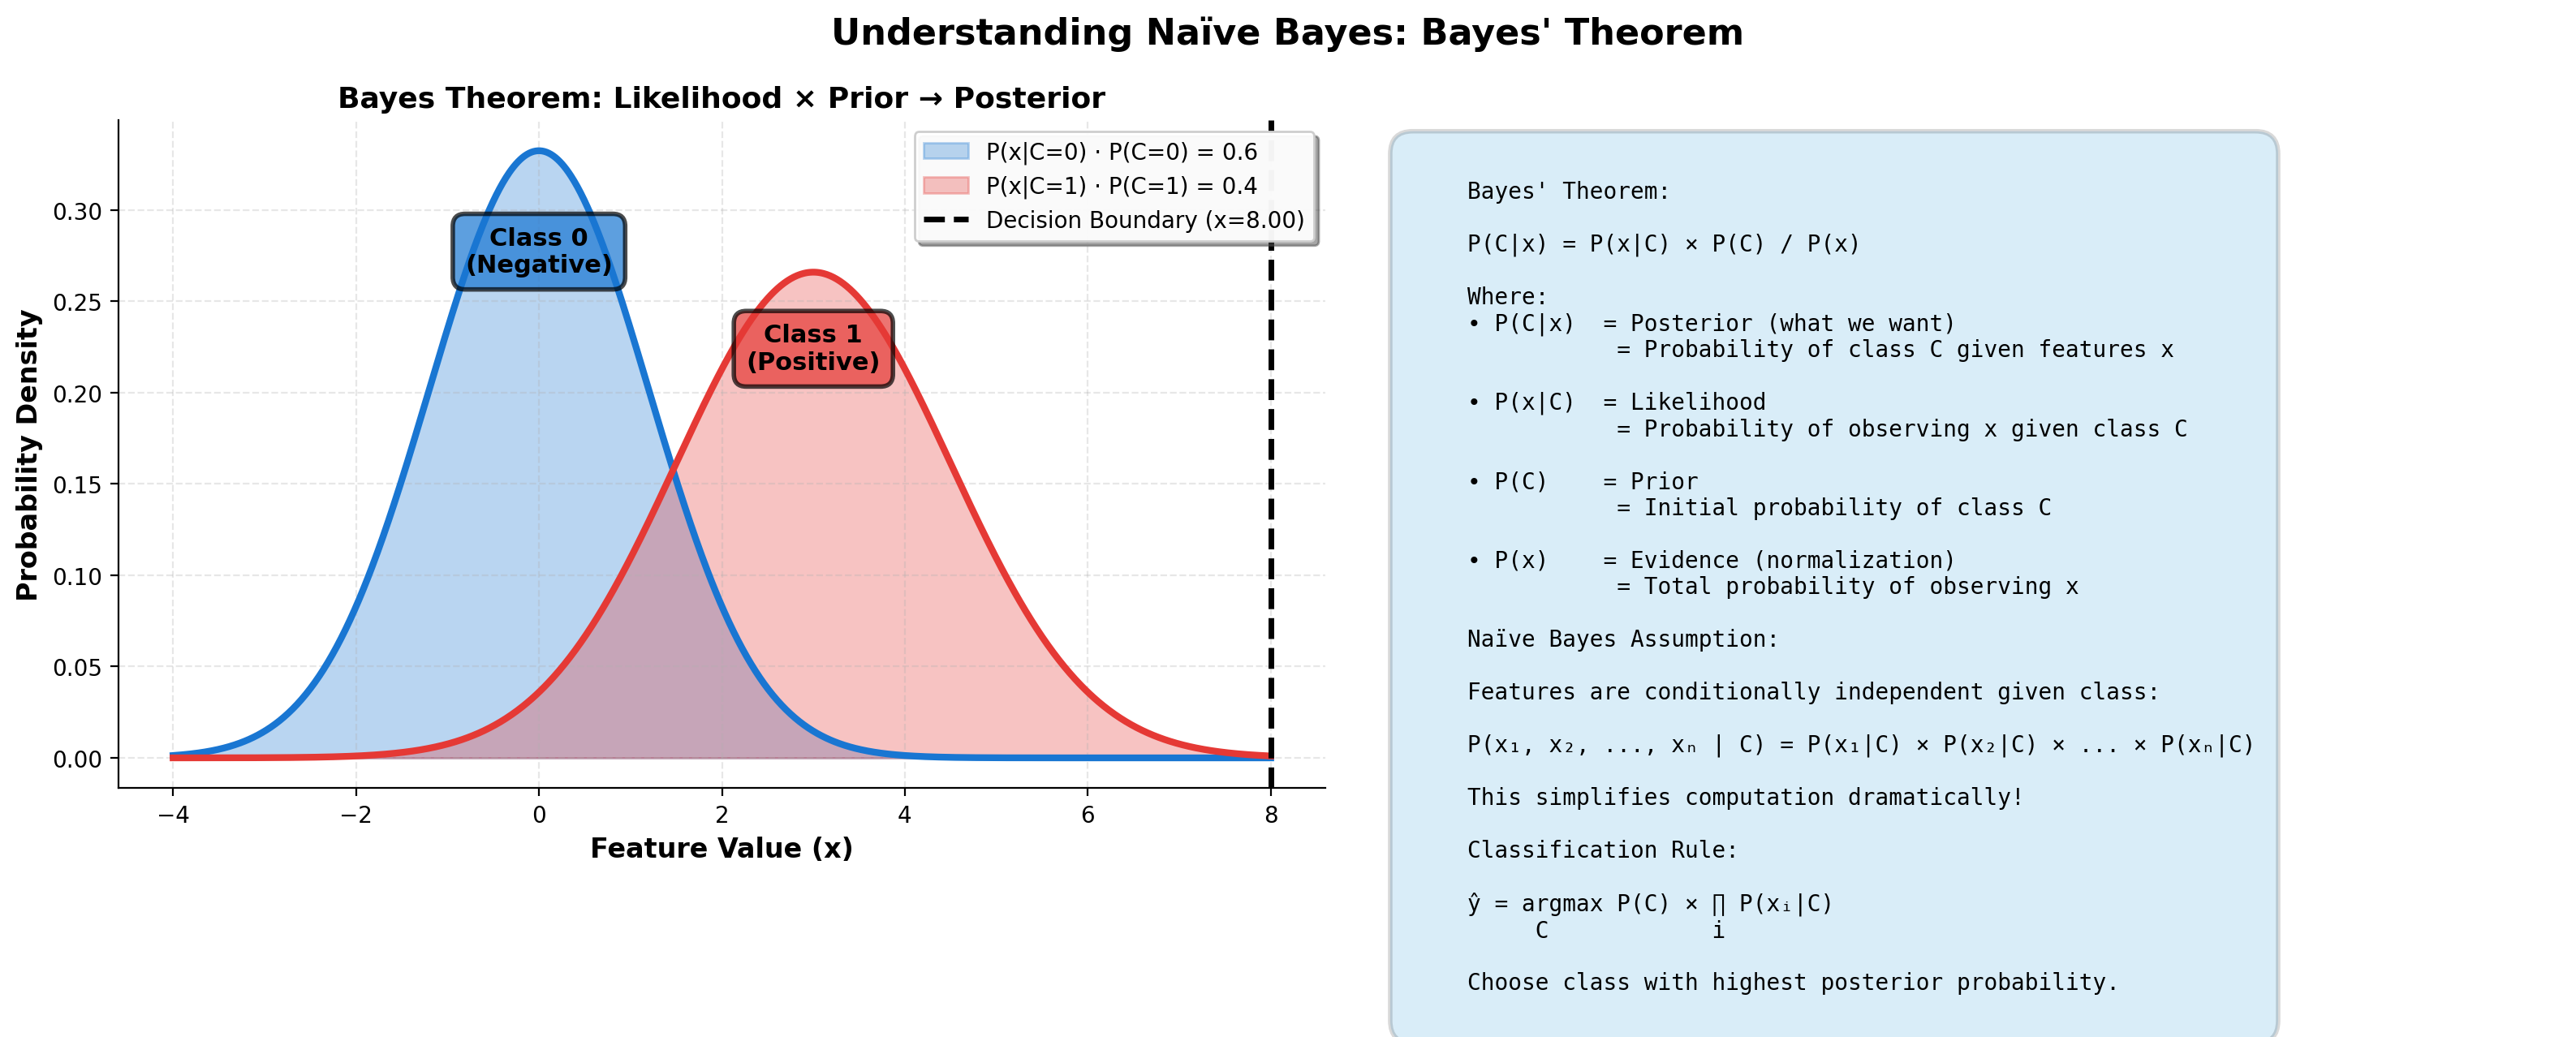
\includegraphics[width=0.75\textwidth]{../figures/nb_bayes_theorem.png}

\vspace{0.1cm}

\begin{alertblock}{Classification Rule}
Choose class with highest posterior: $\hat{y} = \arg\max_{k} P(C_k | \mathbf{x})$
\end{alertblock}
\end{frame}

\begin{frame}{The "Naive" Assumption}

\begin{columns}[t]
\begin{column}{0.52\textwidth}
\begin{block}{Feature Independence}
\textbf{Assumption:} Features are conditionally independent given the class:

$$P(\mathbf{x} | C_k) = P(x_1, x_2, \ldots, x_d | C_k)$$
$$= P(x_1|C_k) \cdot P(x_2|C_k) \cdots P(x_d|C_k)$$
$$= \prod_{i=1}^{d} P(x_i | C_k)$$
\end{block}

\vspace{0.1cm}

\begin{exampleblock}{Why "Naive"?}
This assumption is often violated in practice, but:
\begin{itemize}
\setlength{\itemsep}{1pt}
\item Makes computation tractable
\item Reduces parameters exponentially
\item Works surprisingly well empirically
\end{itemize}
\end{exampleblock}
\end{column}

\begin{column}{0.45\textwidth}
\centering
\vspace{0pt}
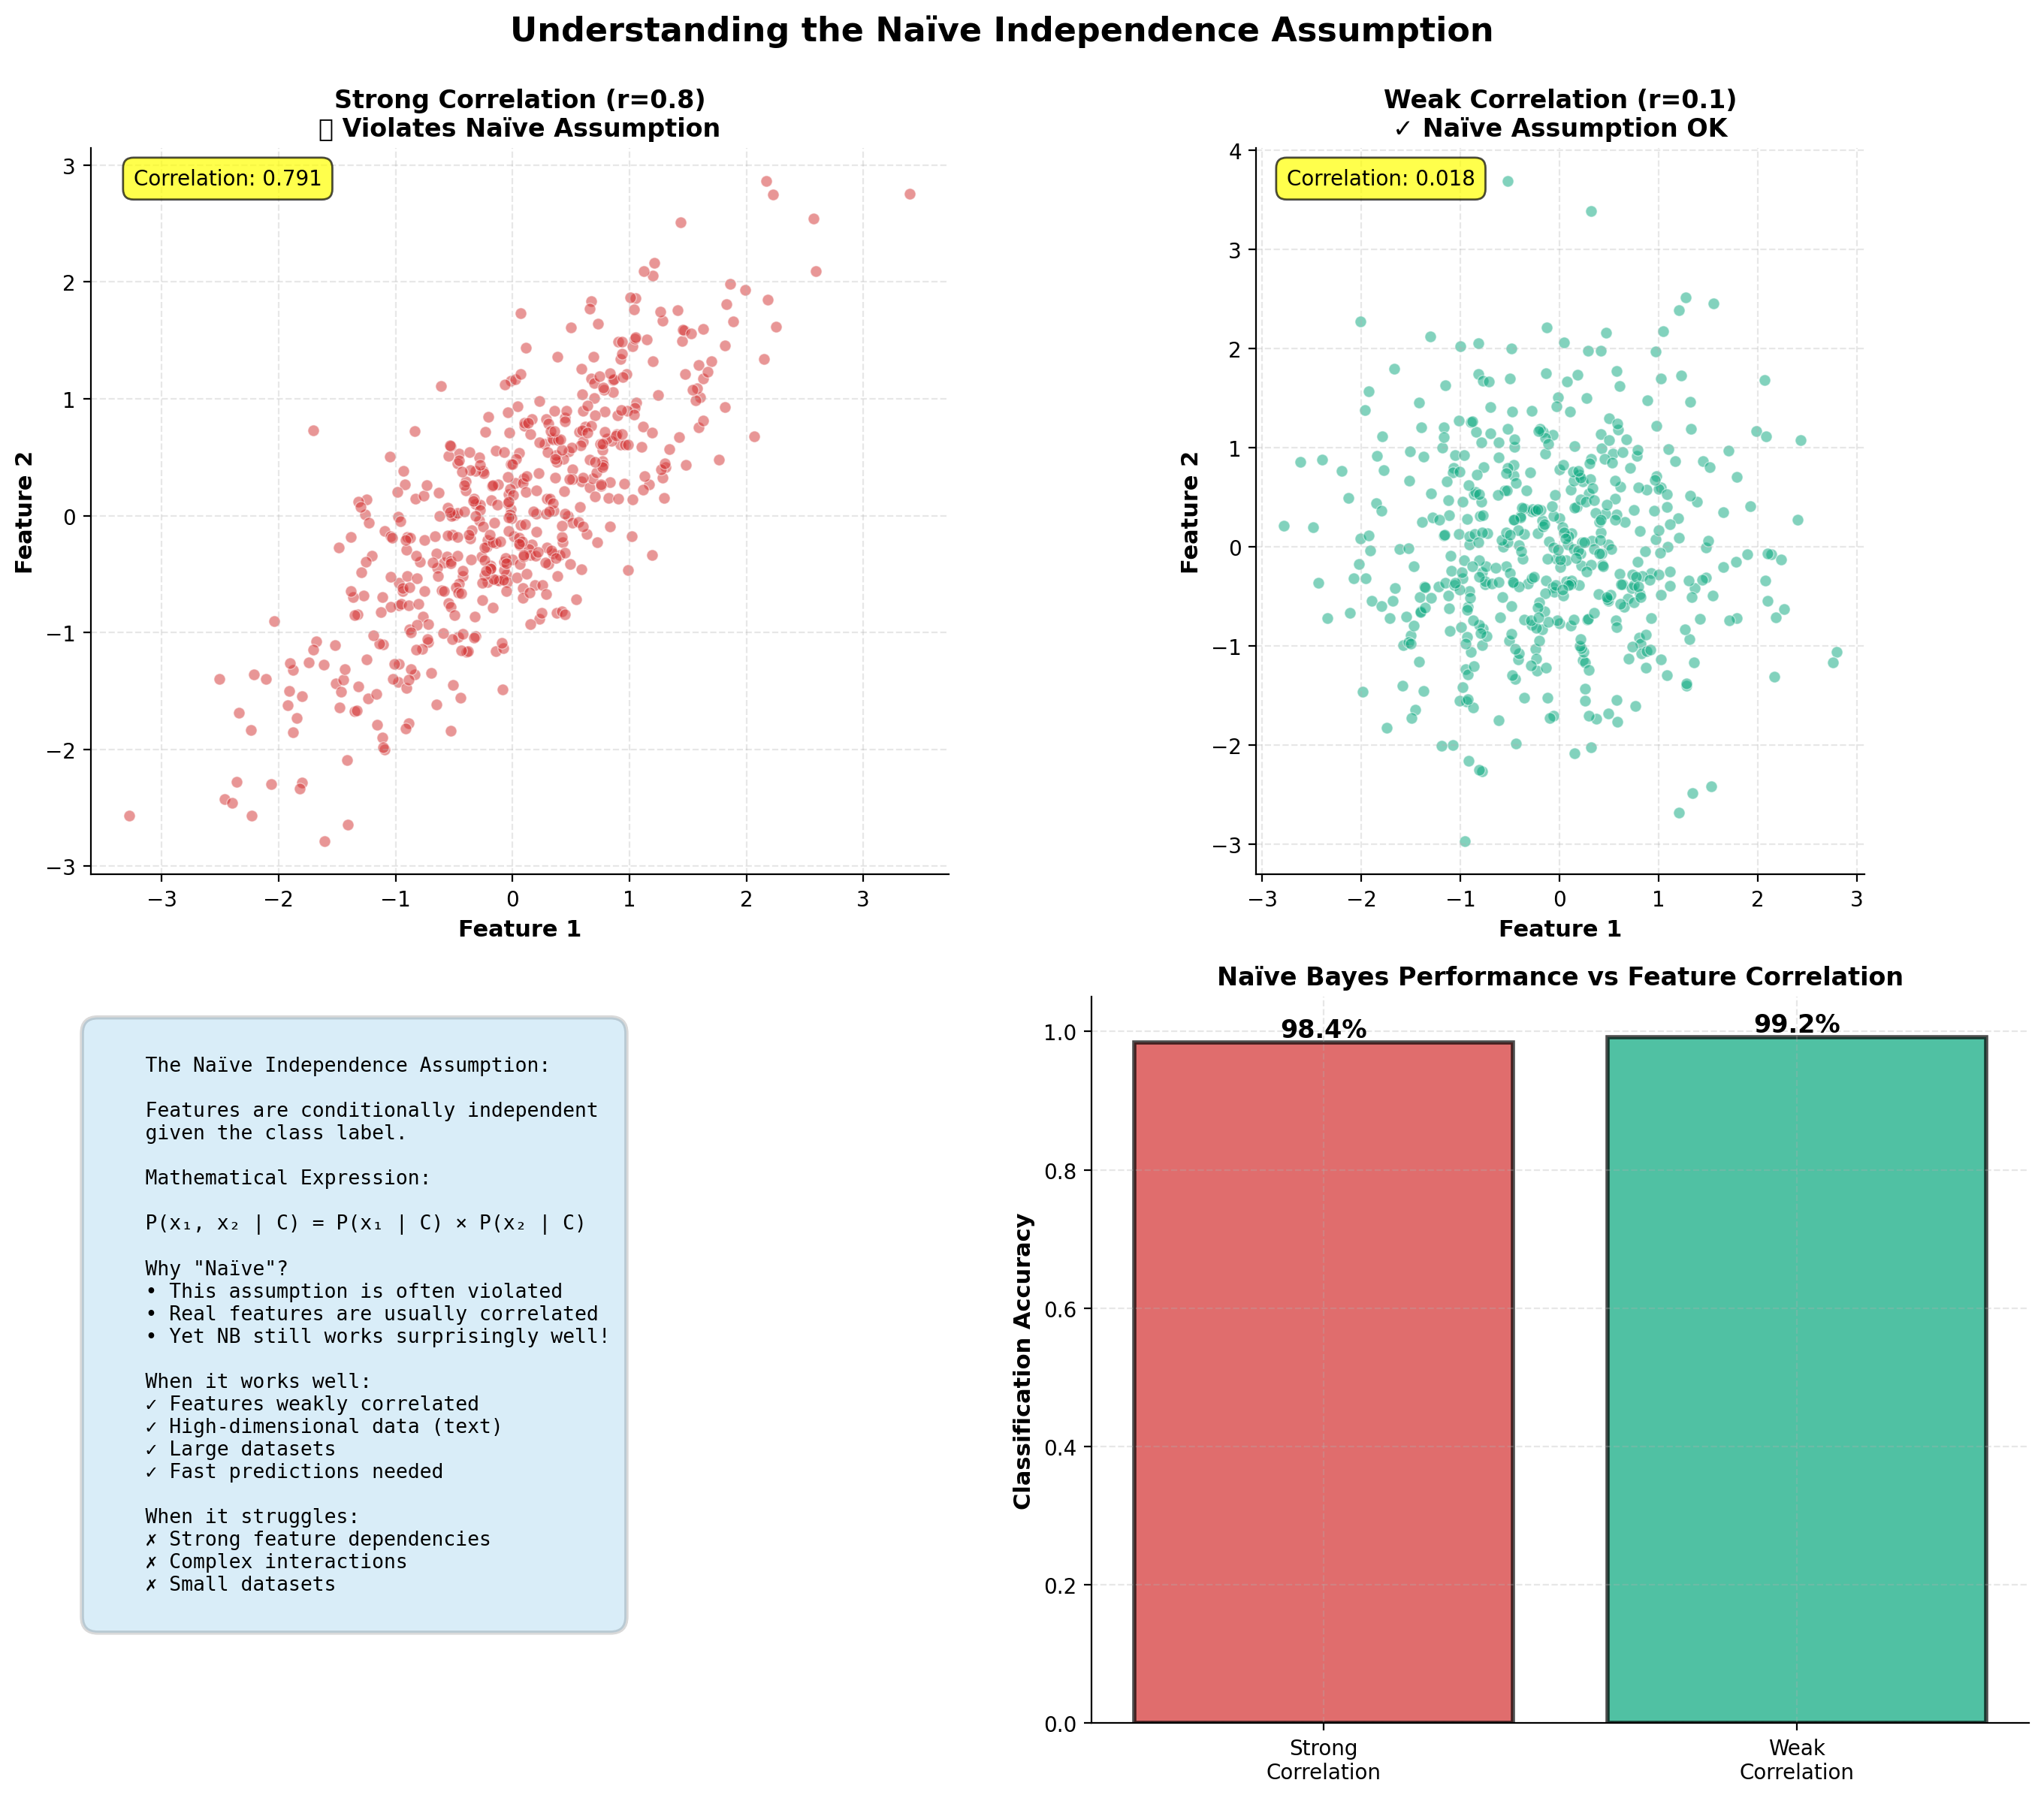
\includegraphics[width=\textwidth]{../figures/nb_naive_assumption.png}

\vspace{0.15cm}

\begin{alertblock}{Practical Impact}
Enables classification with minimal training data and fast prediction!
\end{alertblock}
\end{column}
\end{columns}
\end{frame}

\begin{frame}{Naive Bayes: Classification Formula}

\textbf{Combining Bayes theorem with independence assumption:}

\vspace{0.2cm}

\begin{block}{Full Formula}
$$P(C_k | \mathbf{x}) \propto P(C_k) \prod_{i=1}^{d} P(x_i | C_k)$$

\vspace{0.1cm}

\textbf{Classification decision:}
$$\hat{y} = \arg\max_{k} \left[ P(C_k) \prod_{i=1}^{d} P(x_i | C_k) \right]$$
\end{block}

\vspace{0.15cm}

\begin{exampleblock}{In Practice (Log Probabilities)}
To avoid numerical underflow, use log probabilities:

$$\hat{y} = \arg\max_{k} \left[ \log P(C_k) + \sum_{i=1}^{d} \log P(x_i | C_k) \right]$$
\end{exampleblock}

\vspace{0.1cm}

\begin{alertblock}{Key Insight}
We only need to estimate $P(C_k)$ and $P(x_i | C_k)$ from training data!
\end{alertblock}
\end{frame}

\begin{frame}{Types of Naive Bayes Classifiers}

\begin{block}{1. Gaussian Naive Bayes}
For \textbf{continuous} features: Assume features follow Gaussian distribution

$$P(x_i | C_k) = \frac{1}{\sqrt{2\pi\sigma_{k,i}^2}} \exp\left(-\frac{(x_i - \mu_{k,i})^2}{2\sigma_{k,i}^2}\right)$$

\textbf{Parameters:} Mean $\mu_{k,i}$ and variance $\sigma_{k,i}^2$ for each feature $i$ and class $k$

\textbf{Use cases:} Iris classification, continuous sensor data
\end{block}

\begin{block}{2. Multinomial Naive Bayes}
For \textbf{discrete counts} (e.g., word frequencies): Assume multinomial distribution

$$P(x_i | C_k) = \frac{N_{k,i} + \alpha}{\sum_{j} N_{k,j} + \alpha d}$$

where $N_{k,i}$ = count of feature $i$ in class $k$, $\alpha$ = smoothing parameter

\textbf{Use cases:} Text classification, document categorization
\end{block}

\begin{block}{3. Bernoulli Naive Bayes}
For \textbf{binary} features: Assume Bernoulli distribution

$$P(x_i | C_k) = P(i|C_k)^{x_i} \cdot (1 - P(i|C_k))^{(1-x_i)}$$

\textbf{Use cases:} Spam filtering (word present/absent), binary feature sets
\end{block}
\end{frame}

\begin{frame}{Gaussian Naive Bayes: Details}

\begin{columns}[t]
\begin{column}{0.48\textwidth}
\begin{block}{Training (Parameter Estimation)}
For each class $C_k$ and feature $i$:

\vspace{0.1cm}

\textbf{1. Prior probability:}
$$P(C_k) = \frac{n_k}{n}$$
where $n_k$ = number of samples in class $k$

\vspace{0.1cm}

\textbf{2. Mean:}
$$\mu_{k,i} = \frac{1}{n_k} \sum_{\mathbf{x}_j \in C_k} x_{j,i}$$

\vspace{0.1cm}

\textbf{3. Variance:}
$$\sigma_{k,i}^2 = \frac{1}{n_k} \sum_{\mathbf{x}_j \in C_k} (x_{j,i} - \mu_{k,i})^2$$
\end{block}
\end{column}

\begin{column}{0.48\textwidth}
\begin{block}{Prediction}
For new sample $\mathbf{x}$:

\vspace{0.1cm}

\textbf{1. Compute log-likelihood for each class:}
$$\log P(C_k | \mathbf{x}) = \log P(C_k)$$
$$+ \sum_{i=1}^{d} \log P(x_i | C_k)$$

\vspace{0.1cm}

\textbf{2. Choose class with highest value:}
$$\hat{y} = \arg\max_{k} \log P(C_k | \mathbf{x})$$
\end{block}

\vspace{0.1cm}

\centering
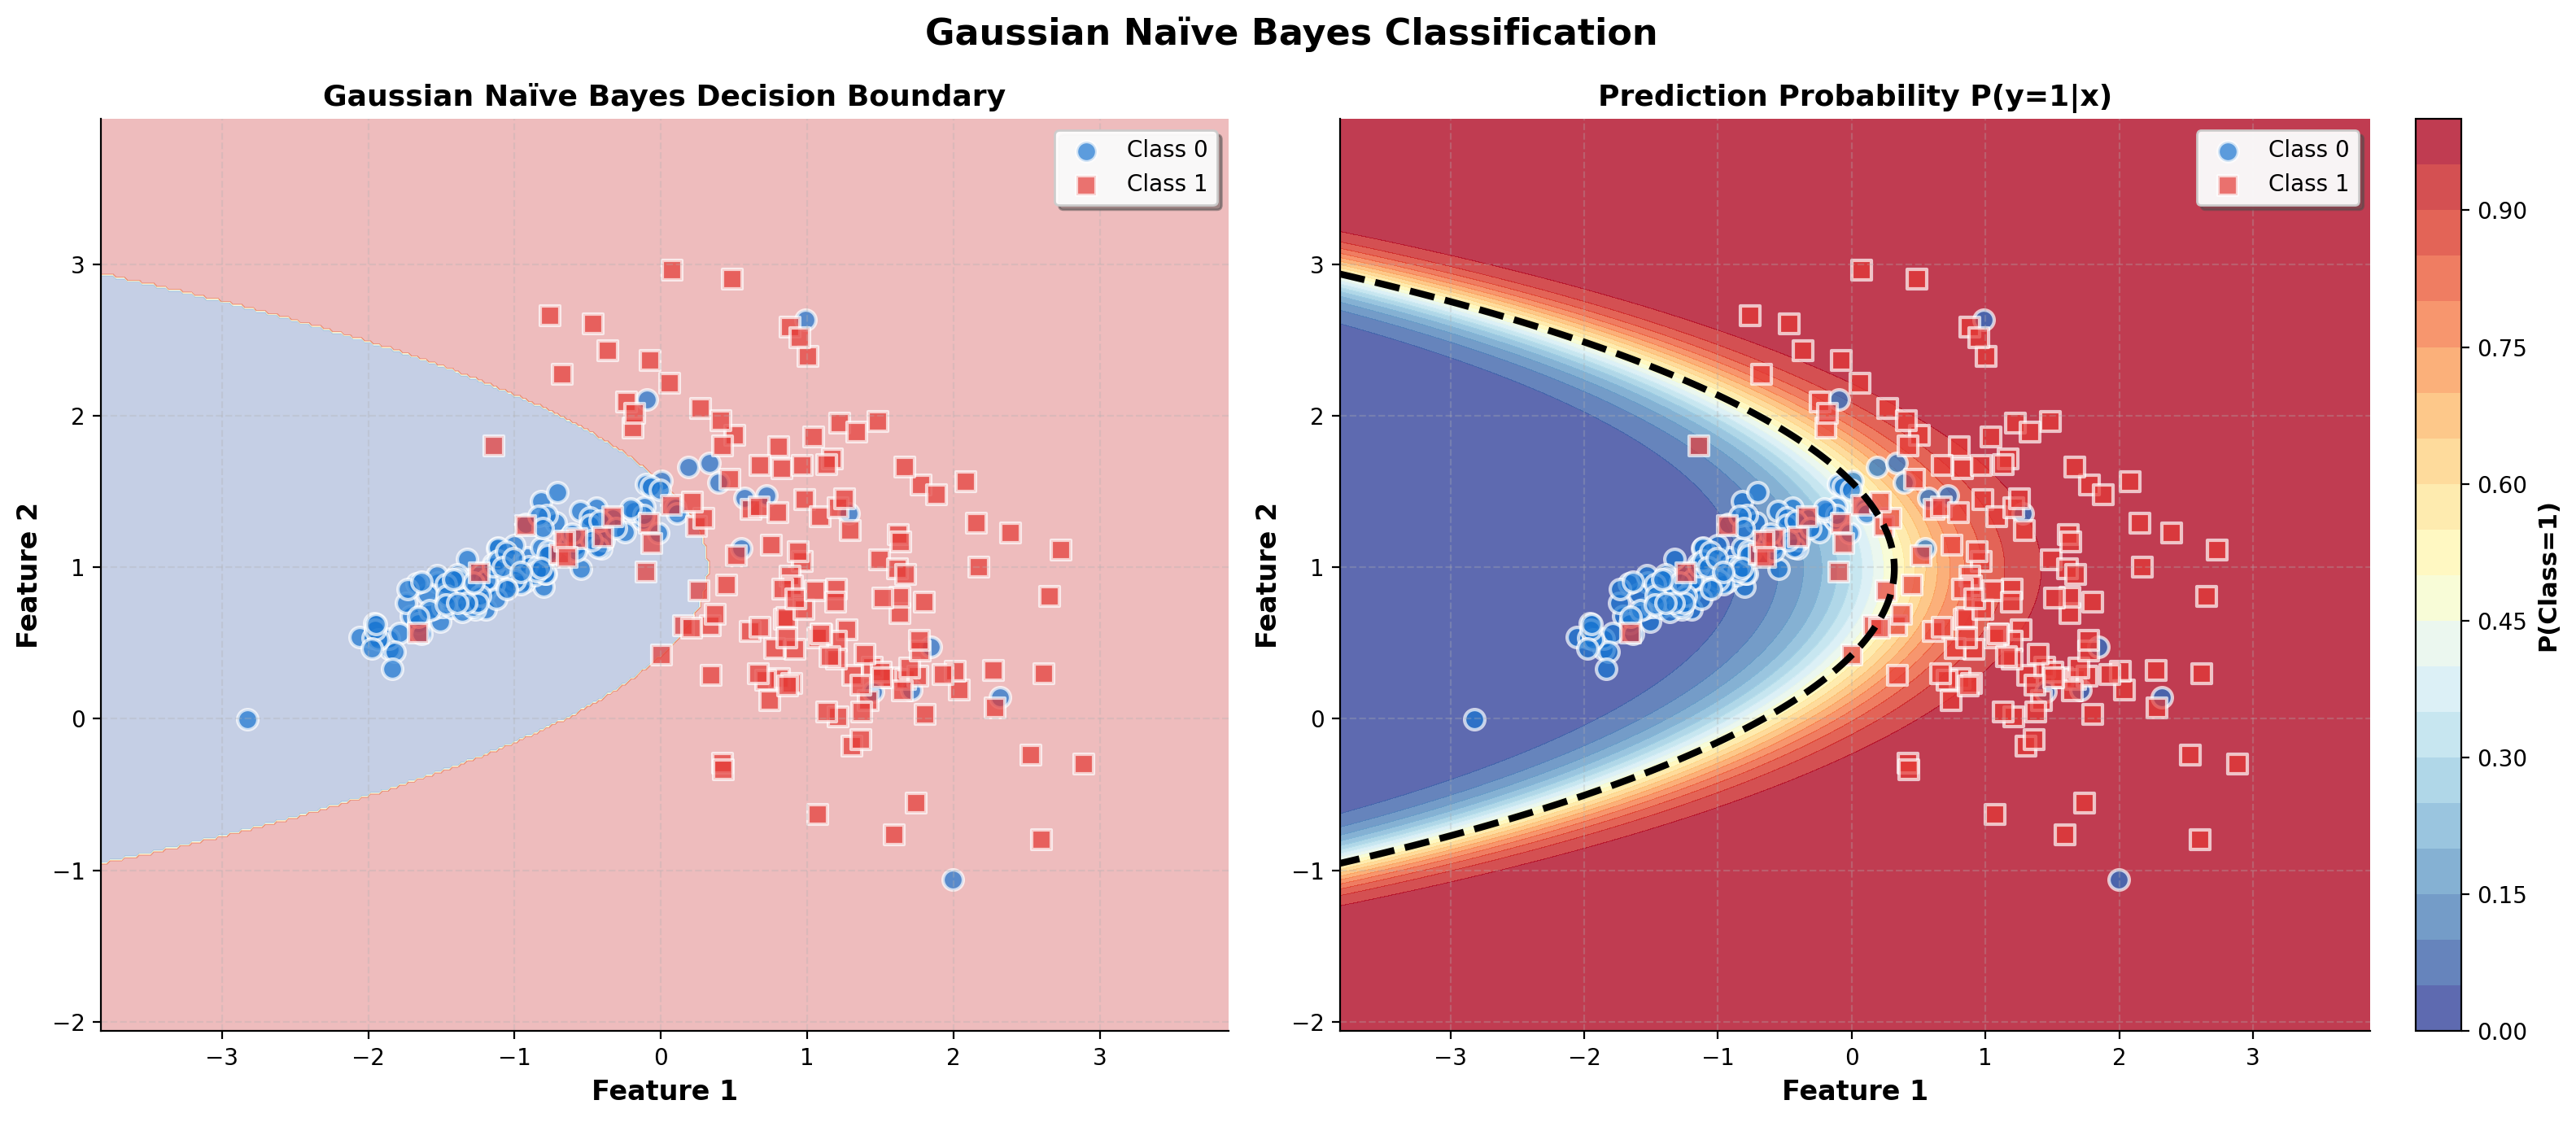
\includegraphics[width=0.95\textwidth]{../figures/nb_gaussian_decision.png}
\end{column}
\end{columns}
\end{frame}

\begin{frame}{Naive Bayes Example: Binary Classification}
\textbf{Dataset: Weather conditions for playing tennis}

\vspace{0.15cm}

\begin{columns}[T]
\begin{column}{0.38\textwidth}
\begin{block}{Training Data}
\small
\begin{tabular}{cccc}
\toprule
Outlook & Temp & Humidity & Play \\
\midrule
Sunny & Hot & High & No \\
Sunny & Hot & High & No \\
Overcast & Hot & High & Yes \\
Rainy & Mild & High & Yes \\
Rainy & Cool & Normal & Yes \\
Rainy & Cool & Normal & No \\
Overcast & Cool & Normal & Yes \\
Sunny & Mild & High & No \\
Sunny & Cool & Normal & Yes \\
\bottomrule
\end{tabular}
\end{block}

\vspace{0.05cm}

\begin{exampleblock}{Question}
Predict: Outlook=Sunny, Temp=Cool, Humidity=High
\end{exampleblock}
\end{column}

\begin{column}{0.60\textwidth}
\begin{block}{Step 1: Compute Priors}
\small
$P(\text{Yes}) = \frac{5}{9} \approx 0.56$ \quad
$P(\text{No}) = \frac{4}{9} \approx 0.44$
\end{block}

\begin{block}{Step 2: Compute Likelihoods}
\small
\textbf{For Class = Yes:}
\begin{itemize}
\setlength{\itemsep}{0pt}
\item $P(\text{Sunny}|\text{Yes}) = \frac{2}{5} = 0.40$
\item $P(\text{Cool}|\text{Yes}) = \frac{3}{5} = 0.60$
\item $P(\text{High}|\text{Yes}) = \frac{1}{5} = 0.20$
\end{itemize}

\textbf{For Class = No:}
\begin{itemize}
\setlength{\itemsep}{0pt}
\item $P(\text{Sunny}|\text{No}) = \frac{2}{4} = 0.50$
\item $P(\text{Cool}|\text{No}) = \frac{1}{4} = 0.25$
\item $P(\text{High}|\text{No}) = \frac{3}{4} = 0.75$
\end{itemize}
\end{block}

\begin{block}{Step 3: Calculate Posteriors}
\small
$P(\text{Yes}|\mathbf{x}) \propto 0.56 \times 0.40 \times 0.60 \times 0.20 = \mathbf{0.027}$

$P(\text{No}|\mathbf{x}) \propto 0.44 \times 0.50 \times 0.25 \times 0.75 = \mathbf{0.041}$

\vspace{0.05cm}

\textbf{Prediction:} \textcolor{red}{\textbf{No}} (higher posterior)
\end{block}
\end{column}
\end{columns}
\end{frame}

\begin{frame}{Naive Bayes: Iris Dataset Example}

\centering
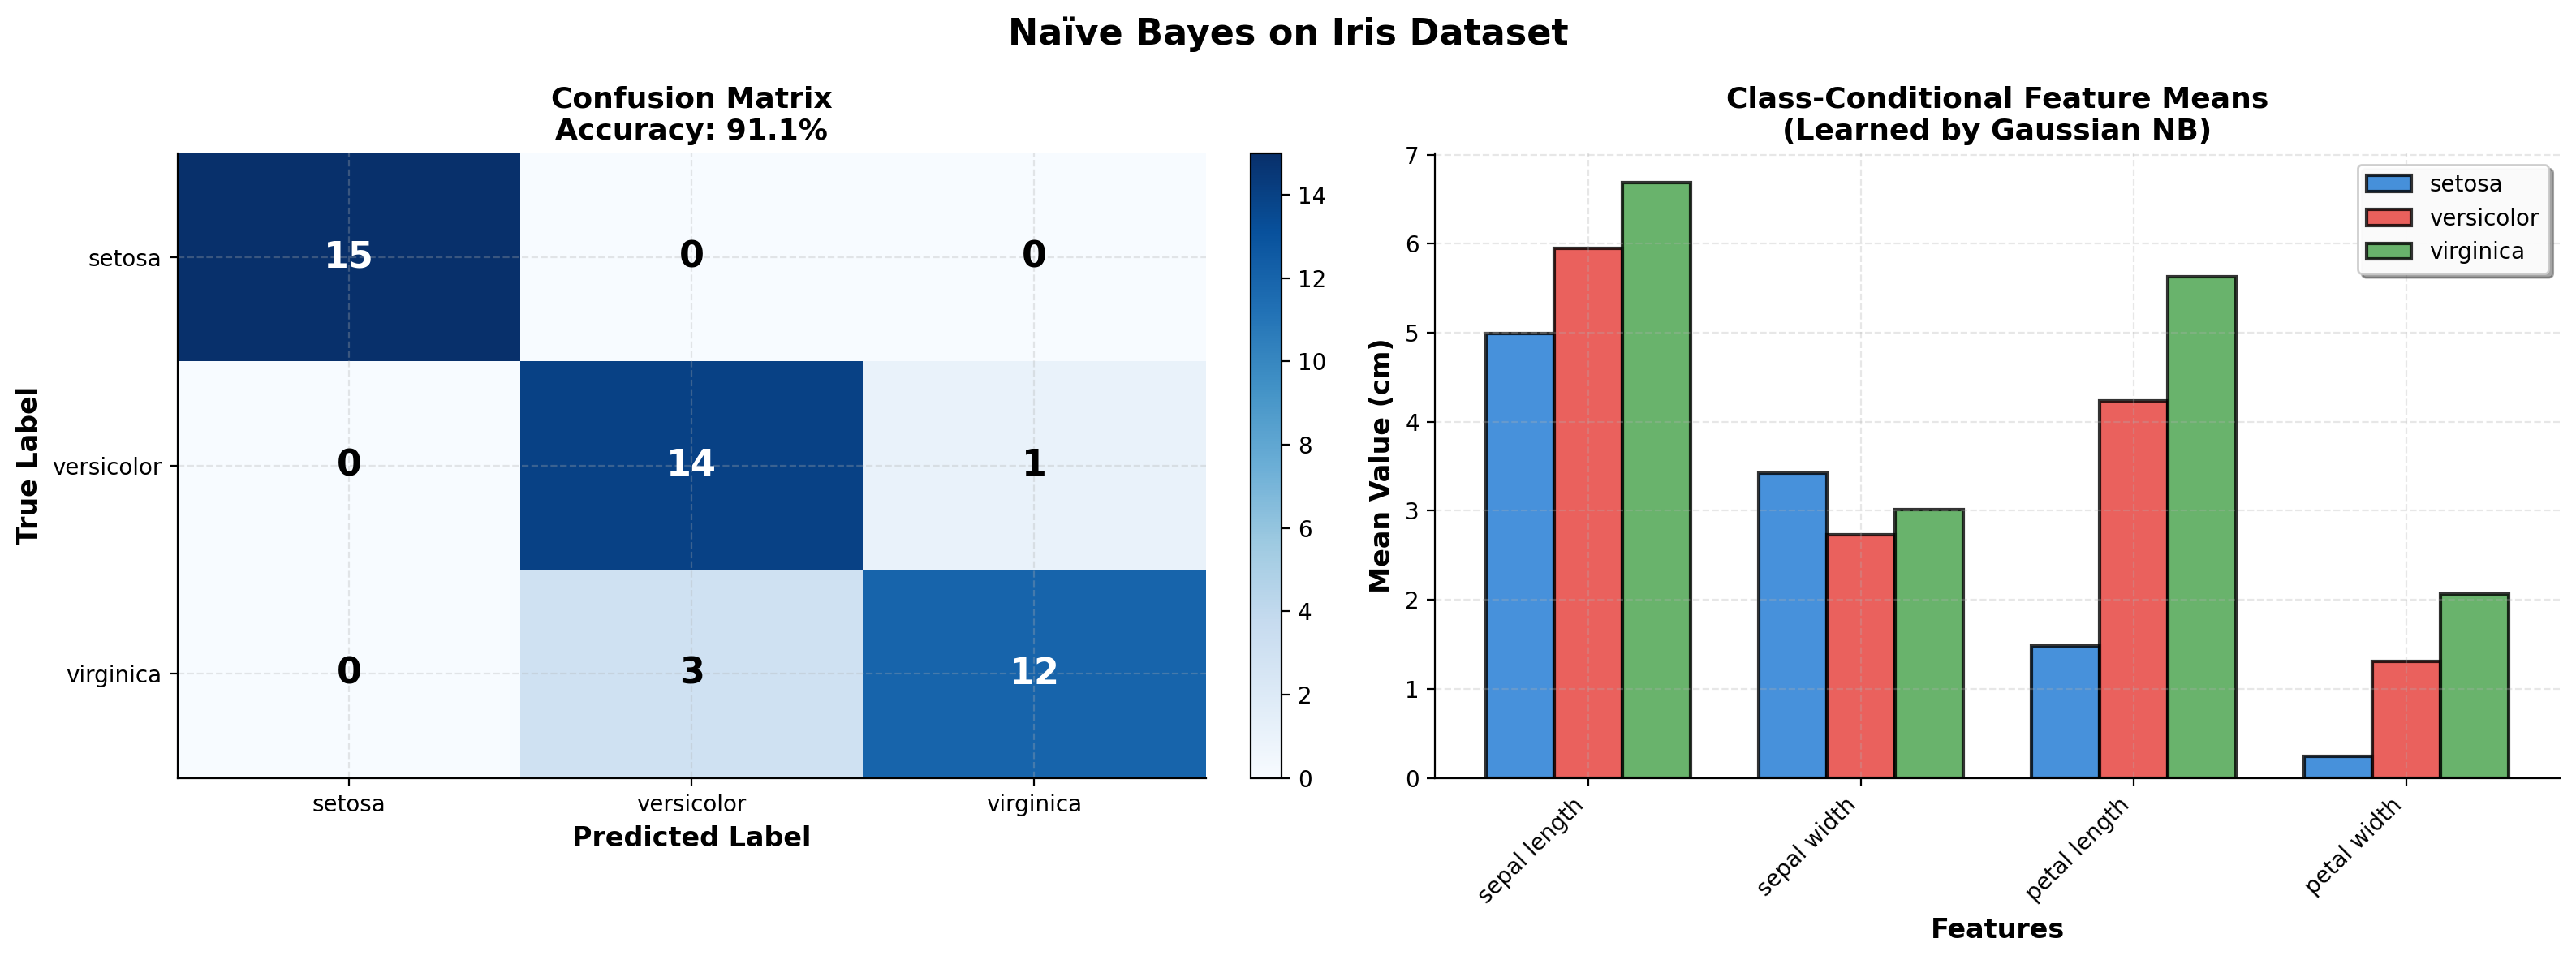
\includegraphics[width=0.95\textwidth]{../figures/nb_iris_example.png}

\vspace{0.1cm}

\begin{columns}[T]
\begin{column}{0.48\textwidth}
\begin{exampleblock}{Gaussian NB Performance}
\begin{itemize}
\setlength{\itemsep}{1pt}
\item \textbf{Training Accuracy:} 96.0\%
\item \textbf{Test Accuracy:} 93.3\%
\item \textbf{Training Time:} $<$1ms
\item \textbf{Prediction Time:} $<$1ms
\end{itemize}
\end{exampleblock}
\end{column}

\begin{column}{0.48\textwidth}
\begin{alertblock}{Key Observations}
\begin{itemize}
\setlength{\itemsep}{1pt}
\item Linear decision boundaries
\item Fast training and prediction
\item Some overlap between classes
\item Good generalization despite naive assumption
\end{itemize}
\end{alertblock}
\end{column}
\end{columns}
\end{frame}

\begin{frame}{Laplace Smoothing}

\begin{alertblock}{Problem: Zero Probabilities}
If a feature value never appears with a class in training: $P(x_i | C_k) = 0$

This makes the entire product zero: $P(C_k | \mathbf{x}) = 0$
\end{alertblock}

\vspace{0.15cm}

\begin{block}{Solution: Laplace (Additive) Smoothing}
Add pseudo-count $\alpha$ (typically $\alpha = 1$):

\vspace{0.1cm}

\textbf{For discrete features:}
$$P(x_i = v | C_k) = \frac{N_{k,v} + \alpha}{N_k + \alpha \cdot V}$$

where:
\begin{itemize}
\item $N_{k,v}$ = count of value $v$ in class $k$
\item $N_k$ = total count in class $k$
\item $V$ = number of unique values for feature $i$
\end{itemize}
\end{block}

\vspace{0.1cm}

\begin{exampleblock}{Effect}
\begin{itemize}
\setlength{\itemsep}{2pt}
\item Prevents zero probabilities
\item Provides small probability to unseen events
\item $\alpha = 1$ called "Laplace smoothing", $\alpha < 1$ called "Lidstone smoothing"
\end{itemize}
\end{exampleblock}
\end{frame}

\begin{frame}[fragile]{Naive Bayes Algorithm (Pseudocode)}

\begin{algorithm}[H]
\caption{Gaussian Naive Bayes}
\begin{algorithmic}[1]
\REQUIRE Training data $\mathcal{D} = \{(\mathbf{x}_1, y_1), \ldots, (\mathbf{x}_n, y_n)\}$
\ENSURE Class prediction for new sample $\mathbf{x}$

\STATE \textbf{Training Phase:}
\FOR{each class $k = 1, \ldots, C$}
    \STATE Compute prior: $P(C_k) = \frac{n_k}{n}$
    \FOR{each feature $i = 1, \ldots, d$}
        \STATE Compute mean: $\mu_{k,i} = \frac{1}{n_k} \sum_{\mathbf{x}_j \in C_k} x_{j,i}$
        \STATE Compute variance: $\sigma_{k,i}^2 = \frac{1}{n_k} \sum_{\mathbf{x}_j \in C_k} (x_{j,i} - \mu_{k,i})^2$
    \ENDFOR
\ENDFOR

\STATE
\STATE \textbf{Prediction Phase:}
\FOR{each class $k = 1, \ldots, C$}
    \STATE $\text{score}_k = \log P(C_k)$
    \FOR{each feature $i = 1, \ldots, d$}
        \STATE $\text{score}_k \mathrel{+}= \log P(x_i | C_k)$ \quad (using Gaussian PDF)
    \ENDFOR
\ENDFOR
\STATE \textbf{return} $\arg\max_k \text{score}_k$
\end{algorithmic}
\end{algorithm}

\vspace{0.05cm}

\begin{alertblock}{Complexity}
\textbf{Training:} $O(nd)$ \quad \textbf{Prediction:} $O(Cd)$ where $C$ = number of classes
\end{alertblock}
\end{frame}

\begin{frame}{Naive Bayes: Advantages \& Disadvantages}

\begin{columns}[t]
\begin{column}{0.48\textwidth}
\begin{block}{Advantages}
\begin{itemize}
\setlength{\itemsep}{3pt}
\item \textbf{Fast:} Training and prediction are very efficient
\item \textbf{Simple:} Easy to understand and implement
\item \textbf{Small data:} Works well with limited training samples
\item \textbf{Multi-class:} Naturally handles multiple classes
\item \textbf{Scalable:} Scales linearly with features and samples
\item \textbf{Probabilistic:} Provides probability estimates
\item \textbf{Online learning:} Can update incrementally
\end{itemize}
\end{block}
\end{column}

\begin{column}{0.48\textwidth}
\begin{block}{Disadvantages}
\begin{itemize}
\setlength{\itemsep}{3pt}
\item \textbf{Independence assumption:} Rarely true in practice
\item \textbf{Zero frequency:} Needs smoothing for unseen values
\item \textbf{Poor estimates:} Probability estimates not always accurate
\item \textbf{Feature correlations:} Cannot capture dependencies
\item \textbf{Continuous data:} Distribution assumption may not hold
\item \textbf{Imbalanced data:} Prior bias with skewed classes
\end{itemize}
\end{block}
\end{column}
\end{columns}

\vspace{0.15cm}

\begin{alertblock}{When to Use Naive Bayes}
\textbf{Good for:} Text classification, spam filtering, real-time prediction, high-dimensional data\\
\textbf{Avoid when:} Feature independence badly violated, need probability calibration
\end{alertblock}
\end{frame}

% ========================================
% Section: K-Nearest Neighbors
% ========================================

\section{K-Nearest Neighbors (KNN)}

\begin{frame}{K-Nearest Neighbors: The Idea}

\begin{columns}[t]
\begin{column}{0.48\textwidth}
\begin{block}{Core Concept}
"You are the average of your $k$ closest neighbors"

\vspace{0.1cm}

\textbf{Classification rule:}
\begin{enumerate}
\setlength{\itemsep}{2pt}
\item Find $k$ nearest training samples
\item Vote based on their labels
\item Assign most common class
\end{enumerate}
\end{block}

\vspace{0.1cm}

\begin{exampleblock}{Key Characteristics}
\begin{itemize}
\setlength{\itemsep}{2pt}
\item \textbf{Non-parametric:} No model to train
\item \textbf{Instance-based:} Stores all training data
\item \textbf{Lazy learning:} Computation at prediction time
\item \textbf{Intuitive:} Easy to understand and visualize
\end{itemize}
\end{exampleblock}
\end{column}

\begin{column}{0.48\textwidth}
\centering
\vspace{0pt}
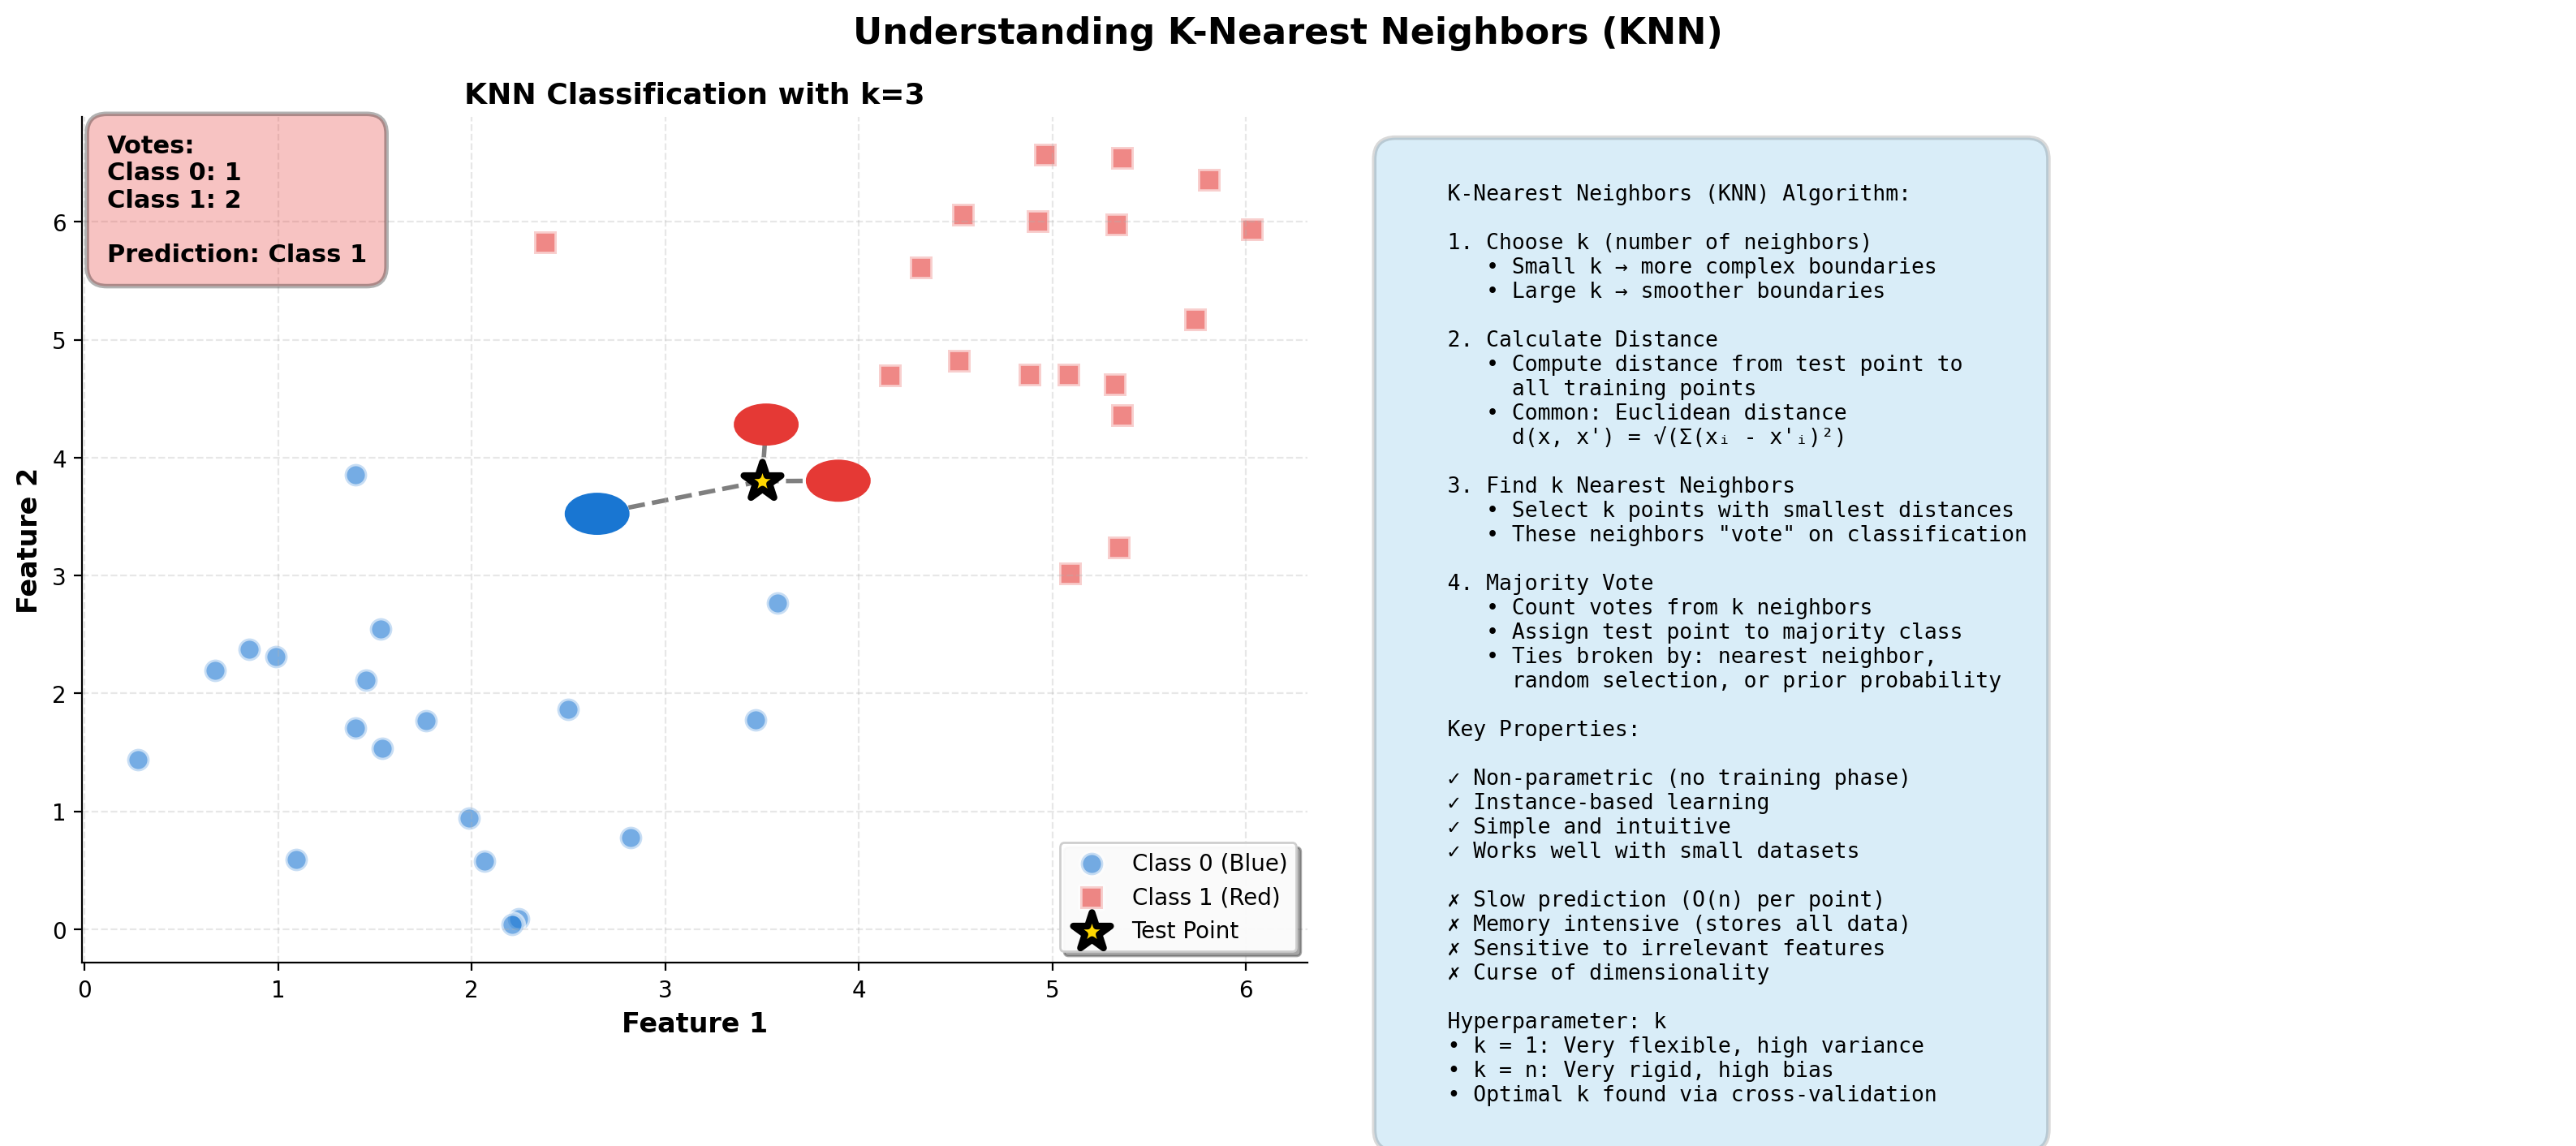
\includegraphics[width=\textwidth]{../figures/knn_concept.png}
\end{column}
\end{columns}

\vspace{0.05cm}

\begin{alertblock}{Intuition}
Similar inputs should have similar outputs!
\end{alertblock}
\end{frame}

\begin{frame}{KNN: Distance Metrics}

\begin{block}{Common Distance Metrics}
For feature vectors $\mathbf{x} = (x_1, \ldots, x_d)$ and $\mathbf{y} = (y_1, \ldots, y_d)$:

\vspace{0.15cm}

\begin{columns}[T]
\begin{column}{0.48\textwidth}
\textbf{1. Euclidean Distance (L2)}
$$d(\mathbf{x}, \mathbf{y}) = \sqrt{\sum_{i=1}^{d} (x_i - y_i)^2}$$

Most common choice, assumes all features equally important

\vspace{0.1cm}

\textbf{2. Manhattan Distance (L1)}
$$d(\mathbf{x}, \mathbf{y}) = \sum_{i=1}^{d} |x_i - y_i|$$

Less sensitive to outliers, good for high dimensions
\end{column}

\begin{column}{0.48\textwidth}
\textbf{3. Minkowski Distance (general)}
$$d(\mathbf{x}, \mathbf{y}) = \left(\sum_{i=1}^{d} |x_i - y_i|^p\right)^{1/p}$$

Generalization: $p=1$ (Manhattan), $p=2$ (Euclidean)

\vspace{0.1cm}

\textbf{4. Chebyshev Distance (L$\infty$)}
$$d(\mathbf{x}, \mathbf{y}) = \max_{i} |x_i - y_i|$$

Maximum difference across any dimension
\end{column}
\end{columns}
\end{block}

\vspace{0.1cm}

\centering
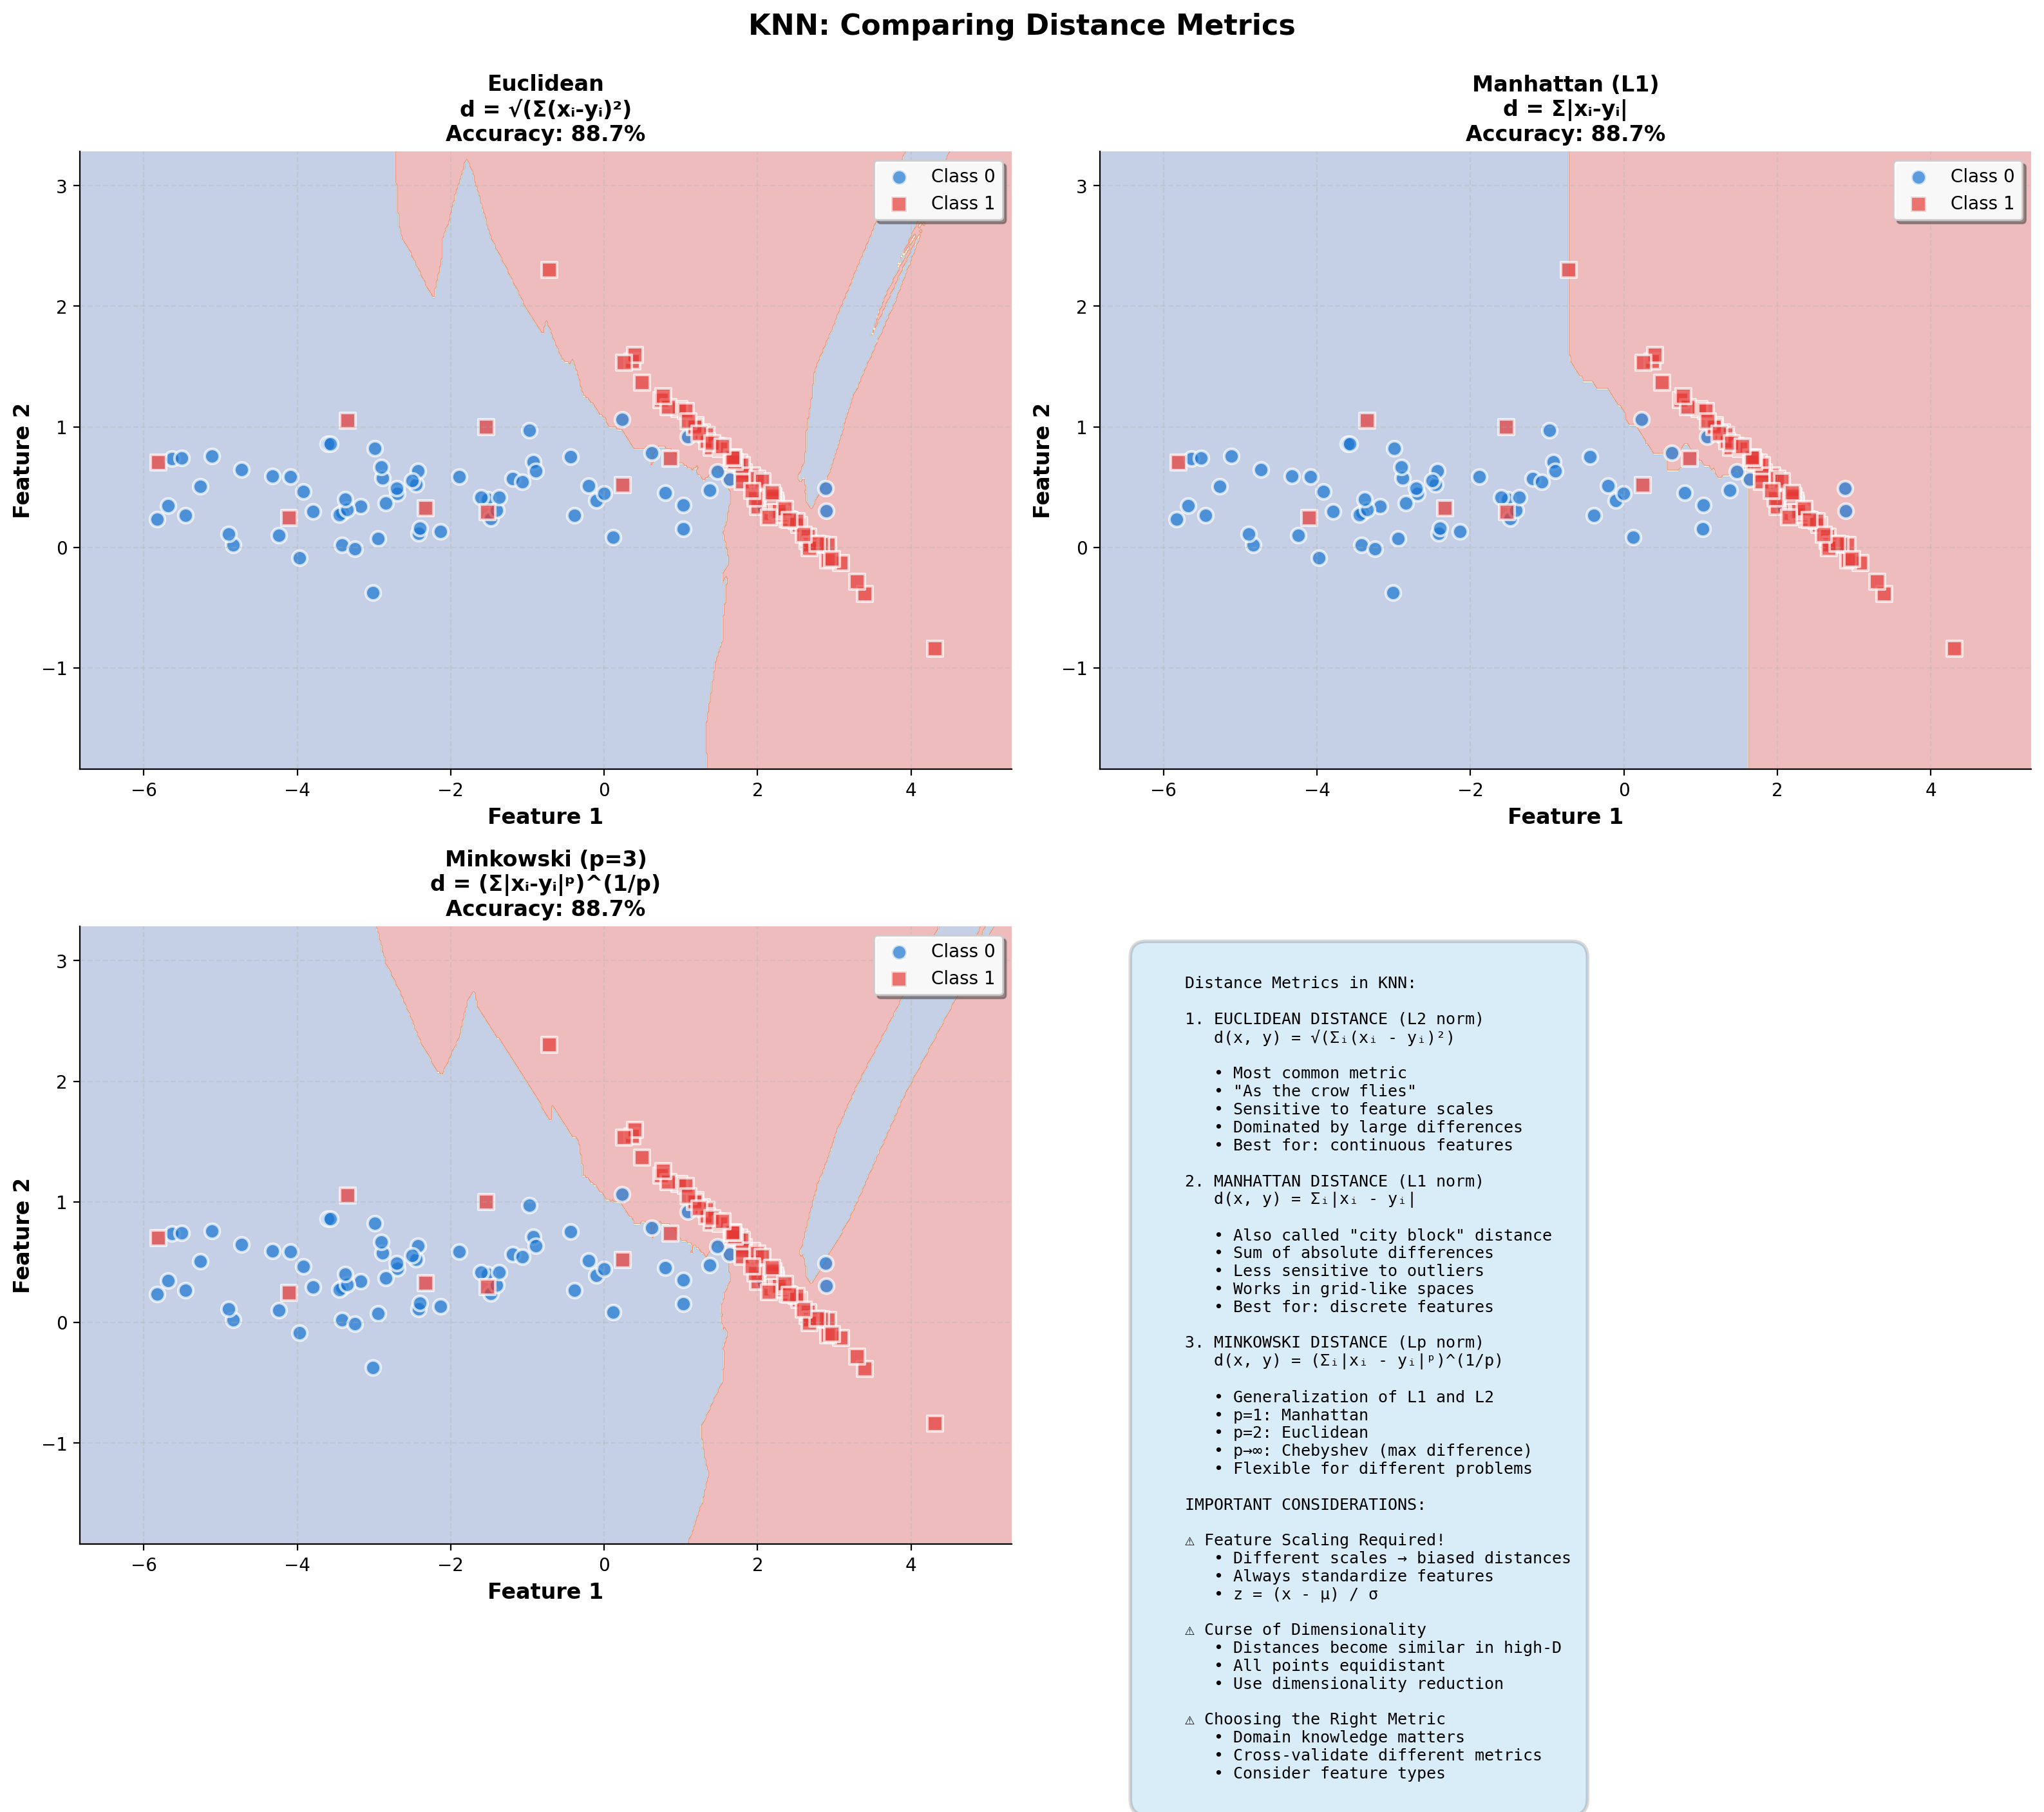
\includegraphics[width=0.75\textwidth]{../figures/knn_distance_metrics.png}
\end{frame}

\begin{frame}[fragile]{KNN Algorithm}

\begin{algorithm}[H]
\caption{K-Nearest Neighbors Classification}
\begin{algorithmic}[1]
\REQUIRE Training data $\mathcal{D} = \{(\mathbf{x}_1, y_1), \ldots, (\mathbf{x}_n, y_n)\}$, parameter $k$, test sample $\mathbf{x}_{\text{test}}$
\ENSURE Predicted class $\hat{y}$

\STATE \textbf{Training Phase:}
\STATE Store all training samples $\mathcal{D}$ \quad (no explicit training!)

\STATE
\STATE \textbf{Prediction Phase:}
\STATE Initialize distance array $D = []$
\FOR{each training sample $(\mathbf{x}_i, y_i)$ in $\mathcal{D}$}
    \STATE Compute distance: $d_i = d(\mathbf{x}_{\text{test}}, \mathbf{x}_i)$
    \STATE Append $(d_i, y_i)$ to $D$
\ENDFOR

\STATE Sort $D$ by distance (ascending)
\STATE Select $k$ nearest neighbors: $N_k = \{(d_1, y_1), \ldots, (d_k, y_k)\}$

\STATE \textbf{Classification (Majority Vote):}
\STATE Count occurrences of each class in $N_k$
\STATE \textbf{return} class with highest count
\end{algorithmic}
\end{algorithm}

\vspace{0.05cm}

\begin{alertblock}{Complexity}
\textbf{Training:} $O(1)$ \quad \textbf{Prediction:} $O(nd)$ per query
\end{alertblock}
\end{frame}

\begin{frame}{KNN Example: Manual Calculation}
\textbf{Binary classification with $k=3$, Euclidean distance}

\vspace{0.15cm}

\begin{columns}[T]
\begin{column}{0.42\textwidth}
\begin{block}{Training Data}
\small
\begin{tabular}{cccc}
\toprule
ID & $x_1$ & $x_2$ & Class \\
\midrule
A & 1 & 2 & Red \\
B & 2 & 3 & Red \\
C & 3 & 1 & Red \\
D & 5 & 4 & Blue \\
E & 5 & 6 & Blue \\
F & 6 & 5 & Blue \\
\bottomrule
\end{tabular}
\end{block}

\vspace{0.1cm}

\begin{exampleblock}{Test Point}
$\mathbf{x}_{\text{test}} = (4, 3)$

Predict class with $k=3$
\end{exampleblock}
\end{column}

\begin{column}{0.56\textwidth}
\begin{block}{Step 1: Compute Distances}
\small
\begin{align*}
d(A) &= \sqrt{(4-1)^2 + (3-2)^2} = \sqrt{10} \approx \mathbf{3.16} \\
d(B) &= \sqrt{(4-2)^2 + (3-3)^2} = \sqrt{4} = \mathbf{2.00} \\
d(C) &= \sqrt{(4-3)^2 + (3-1)^2} = \sqrt{5} \approx \mathbf{2.24} \\
d(D) &= \sqrt{(4-5)^2 + (3-4)^2} = \sqrt{2} \approx \mathbf{1.41} \\
d(E) &= \sqrt{(4-5)^2 + (3-6)^2} = \sqrt{10} \approx 3.16 \\
d(F) &= \sqrt{(4-6)^2 + (3-5)^2} = \sqrt{8} \approx 2.83
\end{align*}
\end{block}

\begin{block}{Step 2: Find 3-Nearest Neighbors}
\small
Sorted: D(1.41), B(2.00), C(2.24), \ldots

\textbf{3 nearest:} D (Blue), B (Red), C (Red)
\end{block}

\begin{block}{Step 3: Majority Vote}
\small
\textbf{Blue:} 1 vote \quad \textbf{Red:} 2 votes

\vspace{0.05cm}

\textbf{Prediction:} \textcolor{red}{\textbf{Red}} (majority class)
\end{block}
\end{column}
\end{columns}
\end{frame}

\begin{frame}{KNN: Choosing K}

\begin{columns}[t]
\begin{column}{0.48\textwidth}
\begin{block}{Effect of K}
\textbf{Small K (e.g., $k=1$):}
\begin{itemize}
\setlength{\itemsep}{1pt}
\item \textbf{Flexible} decision boundary
\item \textbf{Low bias}, high variance
\item Sensitive to noise
\item Prone to overfitting
\end{itemize}

\vspace{0.1cm}

\textbf{Large K (e.g., $k=n$):}
\begin{itemize}
\setlength{\itemsep}{1pt}
\item \textbf{Smooth} decision boundary
\item \textbf{High bias}, low variance
\item More robust to noise
\item Prone to underfitting
\end{itemize}
\end{block}

\vspace{0.05cm}

\begin{alertblock}{Rule of Thumb}
$k = \sqrt{n}$ or use cross-validation
\end{alertblock}
\end{column}

\begin{column}{0.48\textwidth}
\centering
\vspace{0pt}
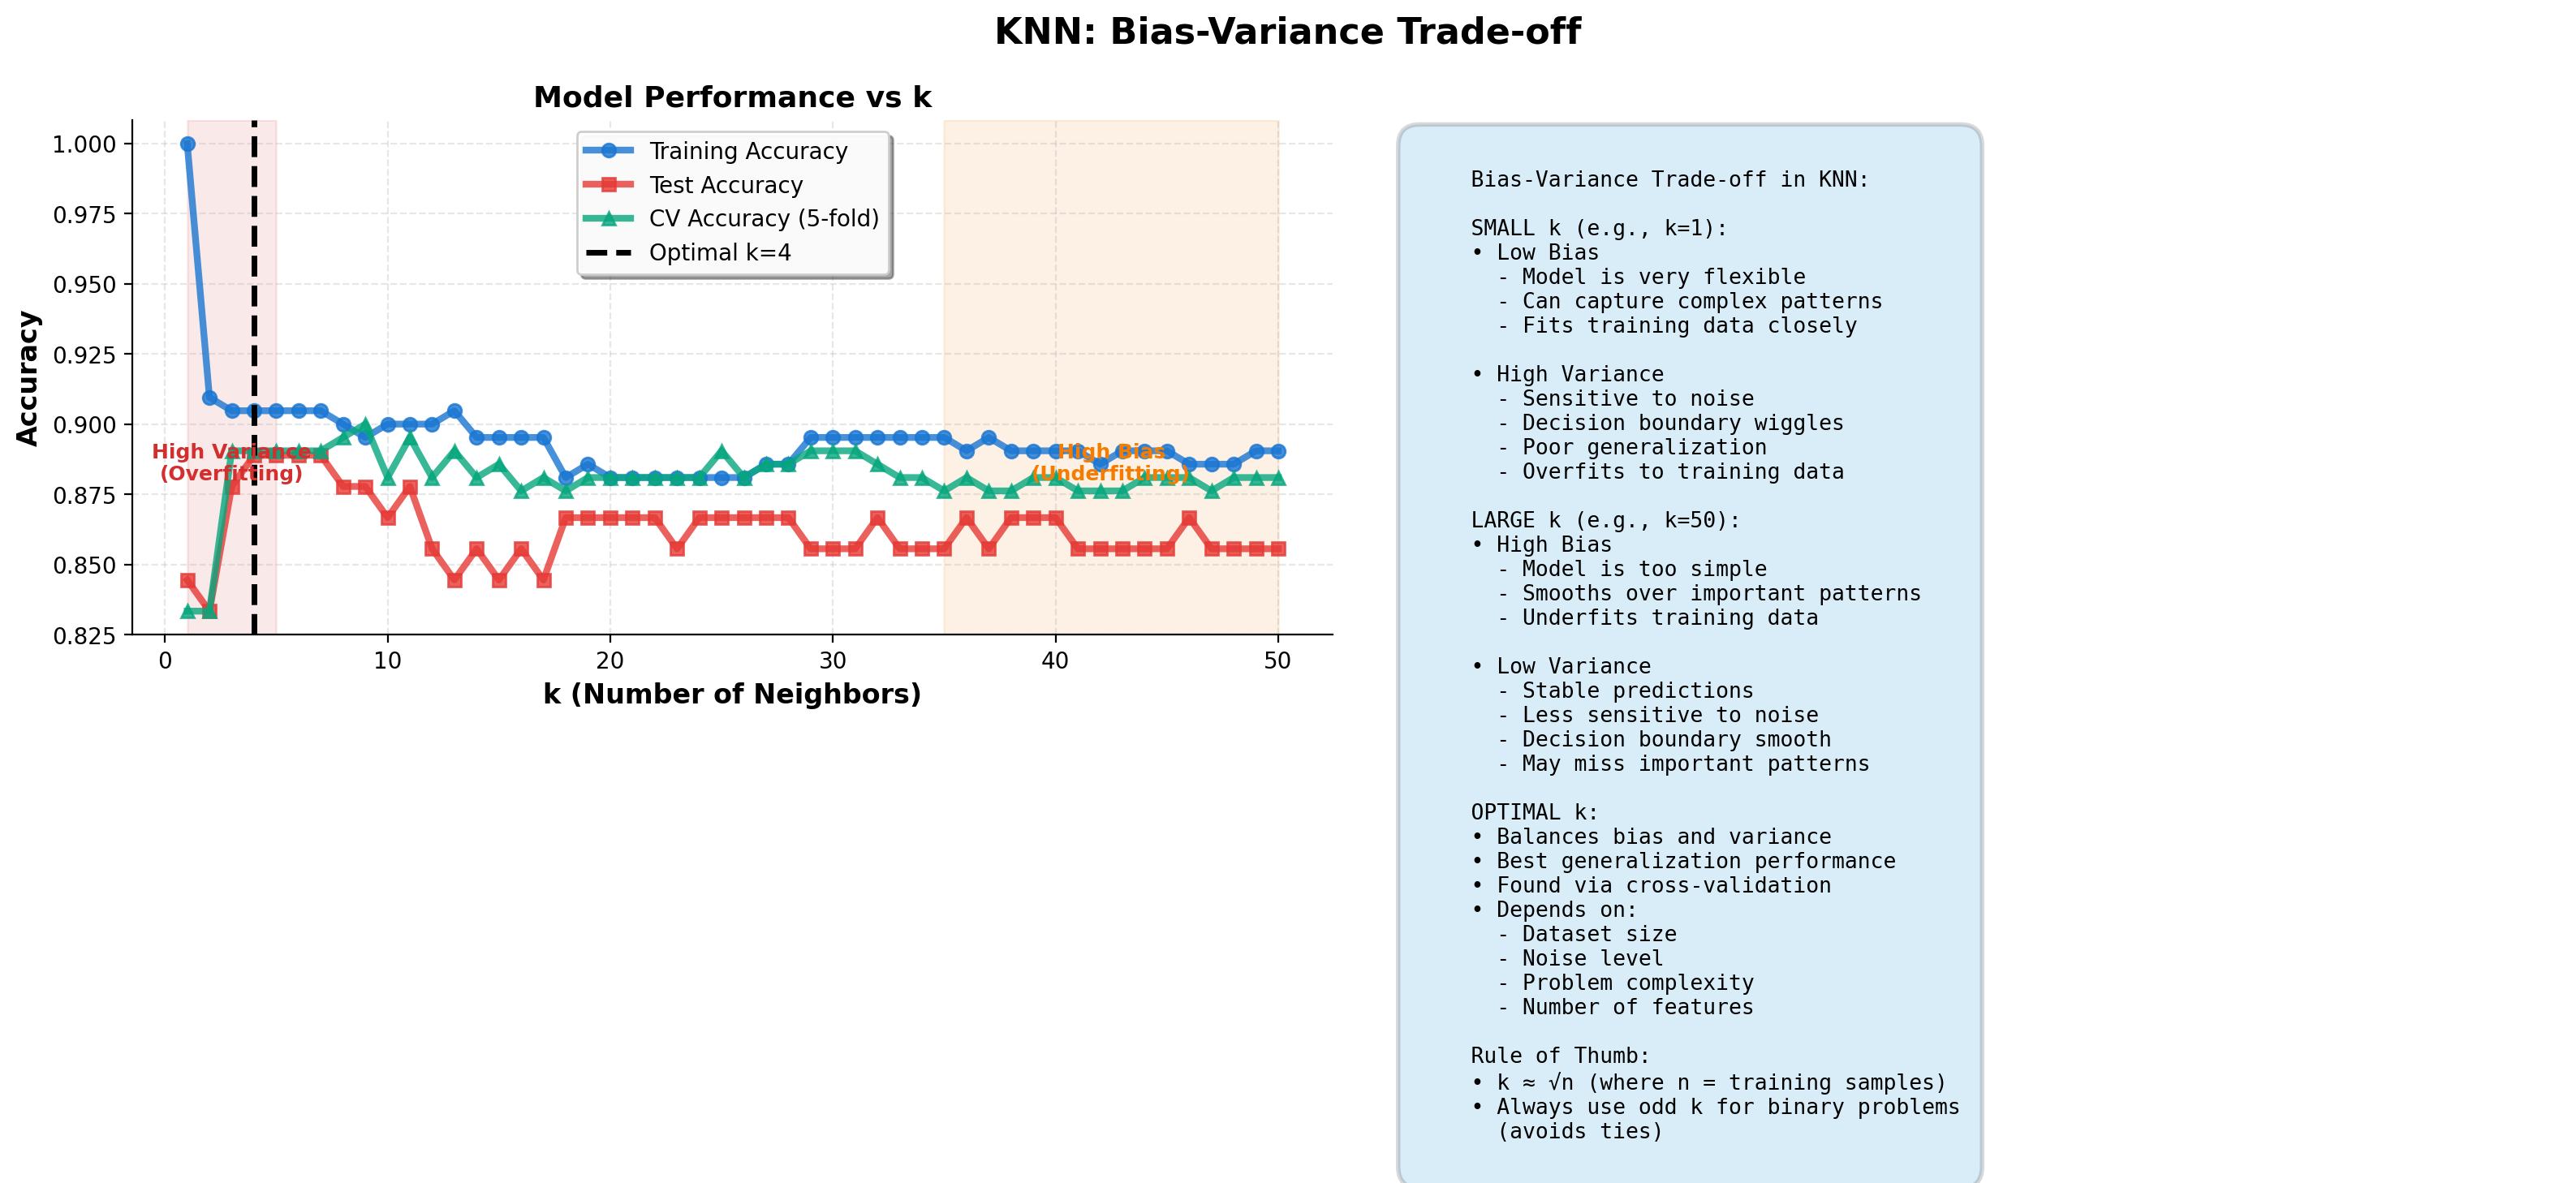
\includegraphics[width=\textwidth]{../figures/knn_bias_variance.png}

\vspace{0.15cm}

\begin{exampleblock}{Best Practice}
\begin{itemize}
\setlength{\itemsep}{2pt}
\item Use \textbf{odd} $k$ for binary classification (avoid ties)
\item Try multiple values: $k \in \{1, 3, 5, 7, 9, \ldots\}$
\item Use cross-validation to select optimal $k$
\item Consider $k \leq 20$ for most problems
\end{itemize}
\end{exampleblock}
\end{column}
\end{columns}
\end{frame}

\begin{frame}{KNN: Decision Boundaries}

\centering
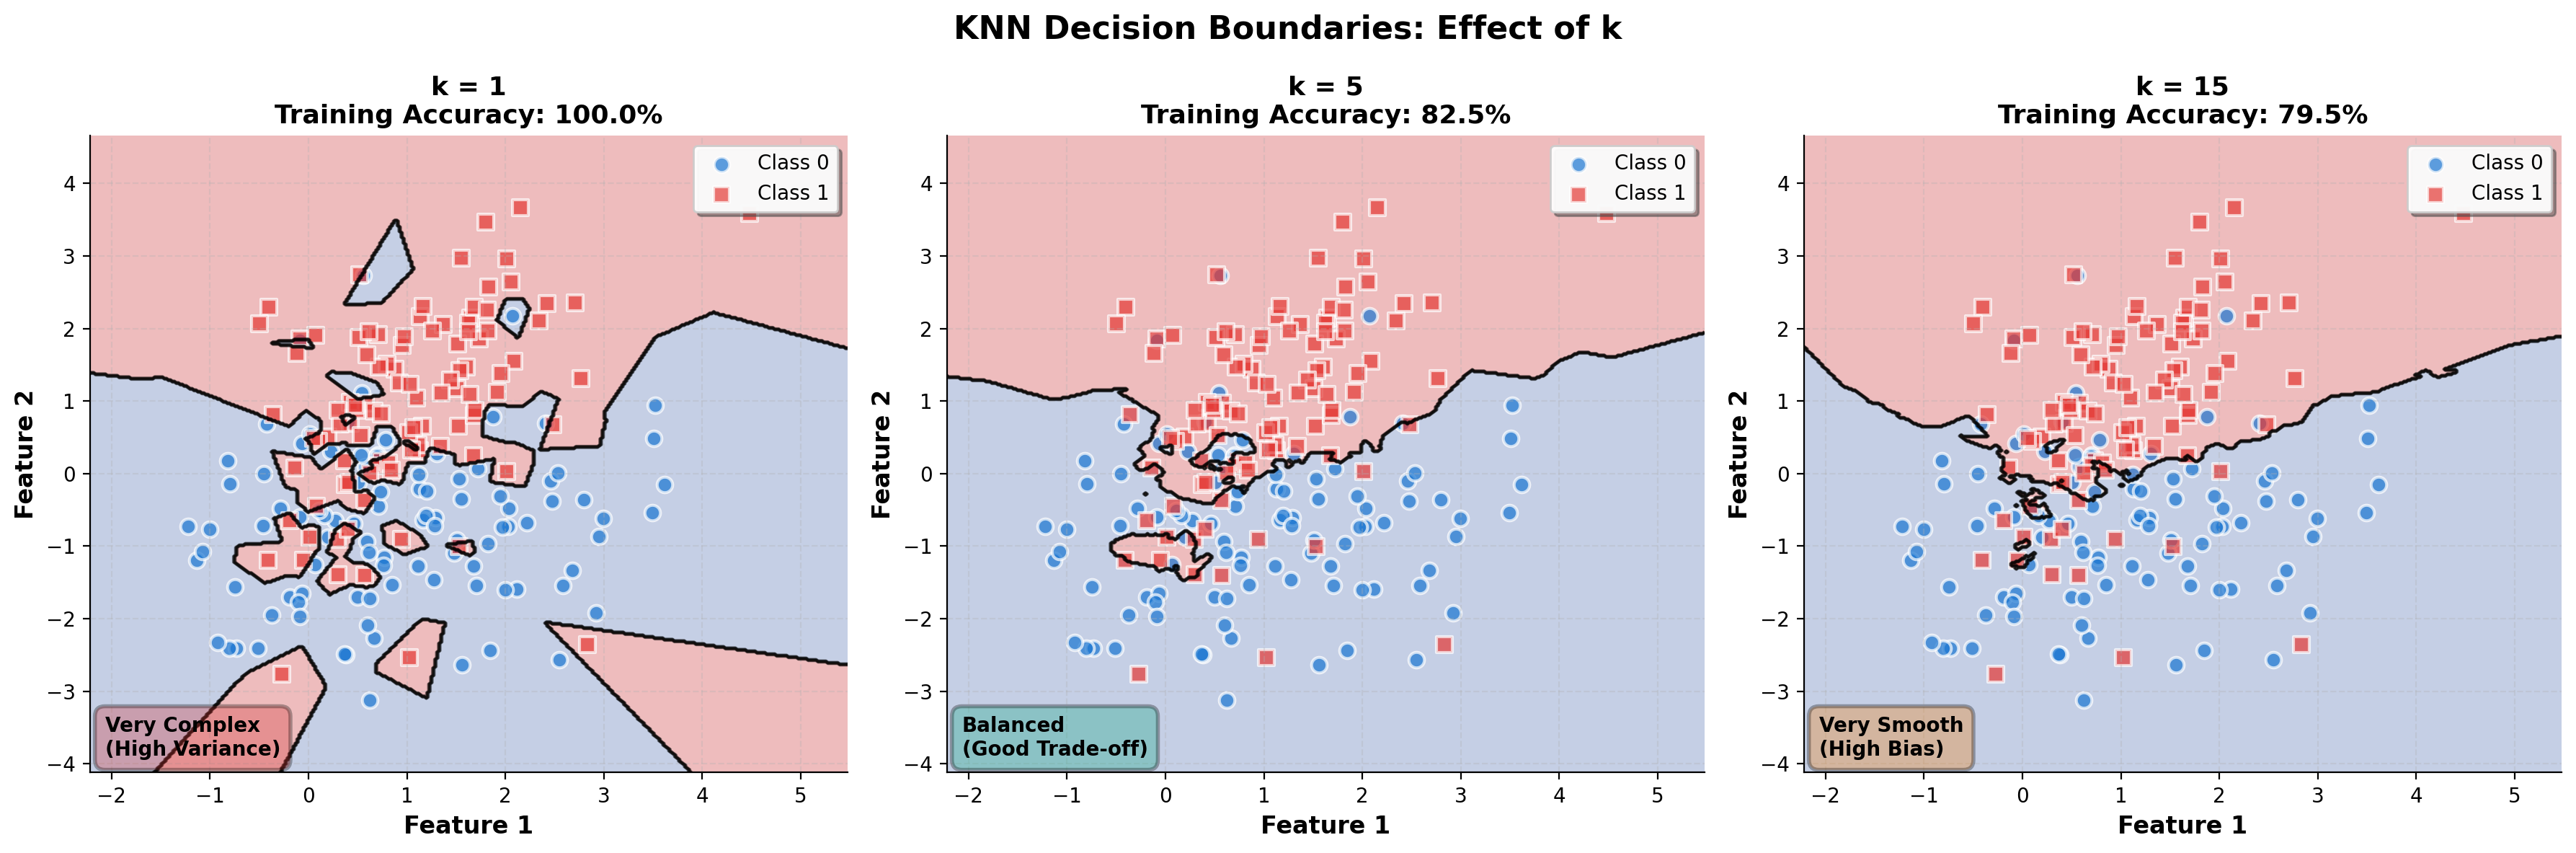
\includegraphics[width=0.95\textwidth]{../figures/knn_decision_boundaries.png}

\vspace{0.1cm}

\begin{columns}[T]
\begin{column}{0.32\textwidth}
\begin{block}{$k=1$}
\begin{itemize}
\setlength{\itemsep}{0pt}
\item Highly irregular
\item Captures all details
\item Overfits training data
\end{itemize}
\end{block}
\end{column}

\begin{column}{0.32\textwidth}
\begin{block}{$k=5$}
\begin{itemize}
\setlength{\itemsep}{0pt}
\item Balanced complexity
\item Smooth but flexible
\item Good generalization
\end{itemize}
\end{block}
\end{column}

\begin{column}{0.32\textwidth}
\begin{block}{$k=15$}
\begin{itemize}
\setlength{\itemsep}{0pt}
\item Very smooth
\item Less flexible
\item May underfit
\end{itemize}
\end{block}
\end{column}
\end{columns}

\vspace{0.05cm}

\begin{alertblock}{Key Insight}
KNN creates \textbf{non-linear} decision boundaries that adapt to local structure!
\end{alertblock}
\end{frame}

\begin{frame}{KNN: Iris Dataset Example}

\centering
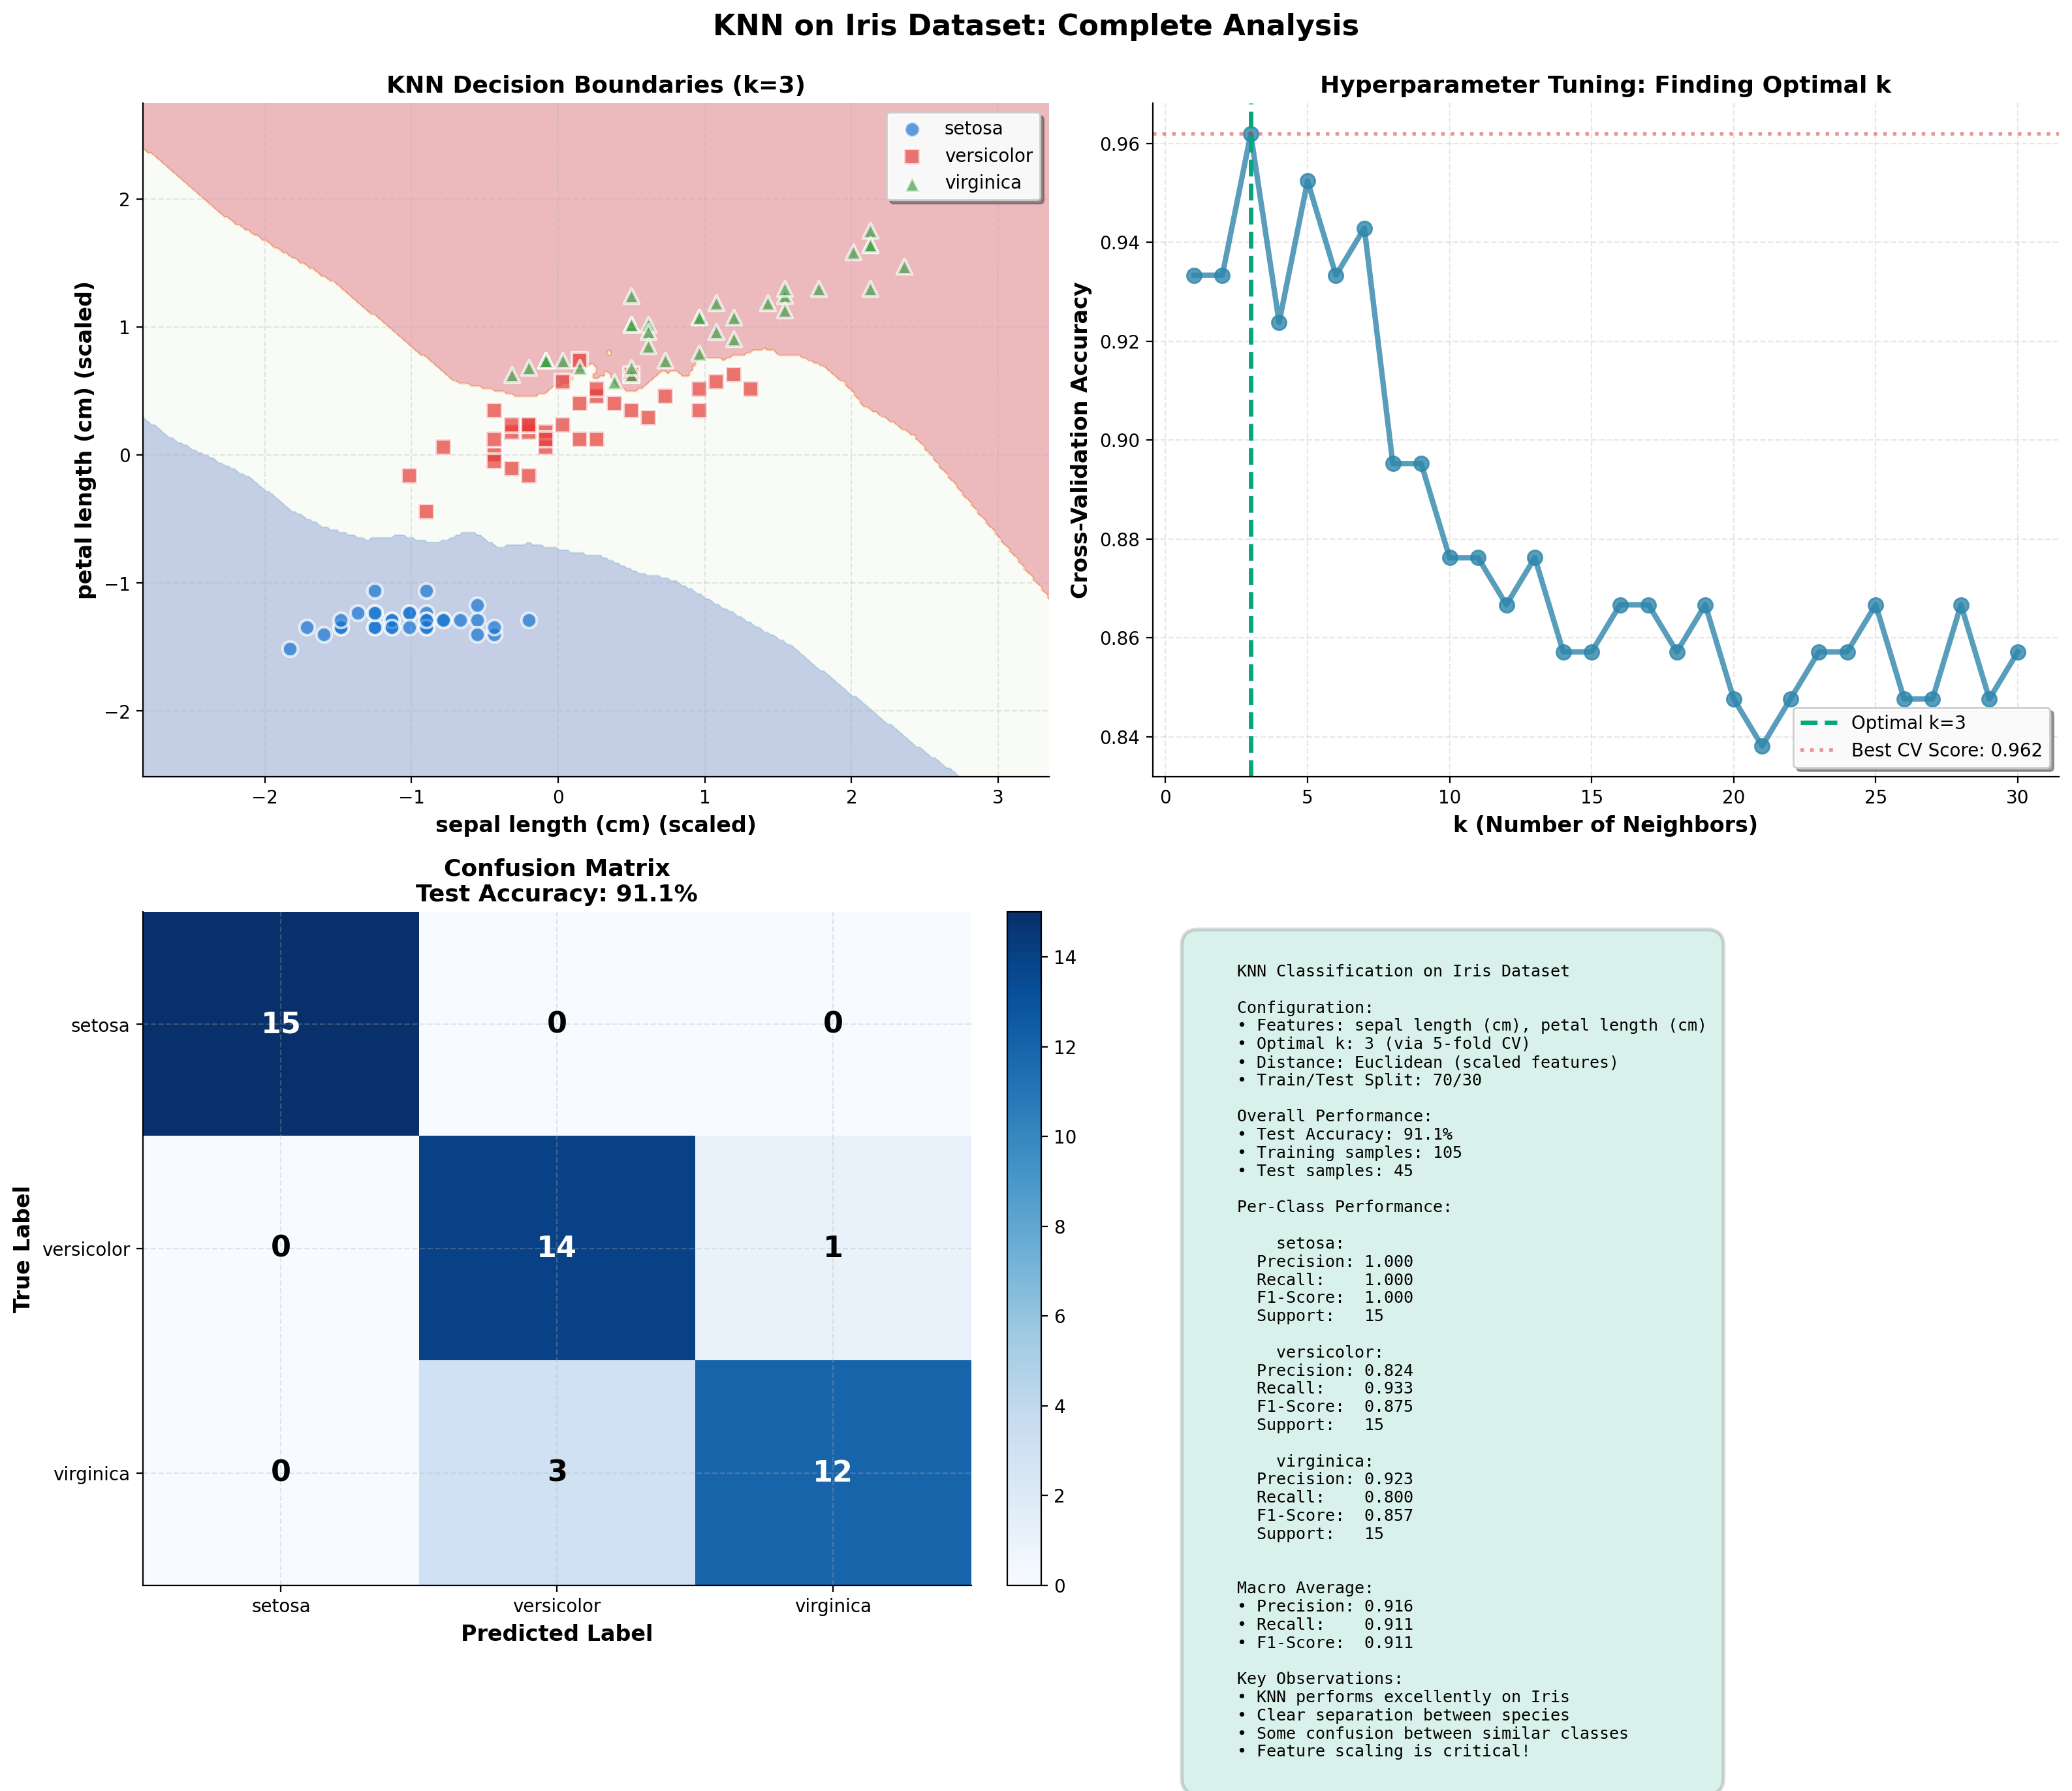
\includegraphics[width=0.95\textwidth]{../figures/knn_iris_example.png}

\vspace{0.05cm}

\begin{columns}[T]
\begin{column}{0.48\textwidth}
\begin{exampleblock}{Performance ($k=5$)}
\begin{itemize}
\setlength{\itemsep}{1pt}
\item \textbf{Training Accuracy:} 96.7\%
\item \textbf{Test Accuracy:} 96.7\%
\item \textbf{Prediction Time:} 2-5ms per sample
\item \textbf{Best $k$:} 5 (via cross-validation)
\end{itemize}
\end{exampleblock}
\end{column}

\begin{column}{0.48\textwidth}
\begin{alertblock}{Key Observations}
\begin{itemize}
\setlength{\itemsep}{1pt}
\item Non-linear decision boundaries
\item Adapts to local data structure
\item Some classification errors at overlap
\item Feature scaling important!
\end{itemize}
\end{alertblock}
\end{column}
\end{columns}
\end{frame}

\begin{frame}{Curse of Dimensionality}

\begin{alertblock}{Problem: Distance Concentration}
In high dimensions, distances between points become similar!

All points appear equidistant $\Rightarrow$ "nearest" neighbors not actually close
\end{alertblock}

\vspace{0.15cm}

\begin{columns}[t]
\begin{column}{0.48\textwidth}
\begin{block}{Why This Happens}
\begin{itemize}
\setlength{\itemsep}{2pt}
\item Volume of hypersphere grows exponentially with $d$
\item Most data lies near surface of hypersphere
\item Ratio of nearest to farthest distance $\rightarrow 1$
\item Need exponentially more data as $d$ increases
\end{itemize}
\end{block}

\vspace{0.1cm}

\begin{exampleblock}{Mitigation Strategies}
\begin{itemize}
\setlength{\itemsep}{2pt}
\item \textbf{Feature selection:} Remove irrelevant features
\item \textbf{Dimensionality reduction:} PCA, feature extraction
\item \textbf{Distance weighting:} Weight by feature importance
\item \textbf{Use appropriate distance:} Manhattan often better in high-d
\end{itemize}
\end{exampleblock}
\end{column}

\begin{column}{0.48\textwidth}
\centering
\vspace{0pt}
\begin{tikzpicture}[scale=1.0]
\begin{axis}[
    xlabel={Number of Dimensions ($d$)},
    ylabel={Samples Needed},
    width=\textwidth,
    height=0.6\textwidth,
    grid=major,
    legend pos=north west,
    ymode=log
]
\addplot[blue, thick, mark=*] coordinates {
    (1, 10) (2, 100) (3, 1000) (4, 10000) (5, 100000)
};
\legend{Training samples}
\end{axis}
\end{tikzpicture}

\vspace{0.15cm}

\begin{alertblock}{Rule of Thumb}
KNN works best with $d < 20$ features
\end{alertblock}
\end{column}
\end{columns}
\end{frame}

\begin{frame}{KNN: Advantages \& Disadvantages}

\begin{columns}[t]
\begin{column}{0.48\textwidth}
\begin{block}{Advantages}
\begin{itemize}
\setlength{\itemsep}{3pt}
\item \textbf{Simple:} Easy to understand and implement
\item \textbf{No training:} No explicit model fitting
\item \textbf{Non-parametric:} No assumptions about data distribution
\item \textbf{Flexible:} Non-linear decision boundaries
\item \textbf{Multi-class:} Naturally handles multiple classes
\item \textbf{Adaptive:} Decision boundary adapts locally
\item \textbf{Incremental:} Easy to add new training data
\end{itemize}
\end{block}
\end{column}

\begin{column}{0.48\textwidth}
\begin{block}{Disadvantages}
\begin{itemize}
\setlength{\itemsep}{3pt}
\item \textbf{Slow prediction:} $O(nd)$ per query
\item \textbf{Memory intensive:} Stores all training data
\item \textbf{Curse of dimensionality:} Poor in high dimensions
\item \textbf{Scaling sensitive:} Must normalize features
\item \textbf{Imbalanced data:} Majority class dominates
\item \textbf{Choosing k:} Requires cross-validation
\item \textbf{No interpretability:} Cannot explain decisions
\end{itemize}
\end{block}
\end{column}
\end{columns}

\vspace{0.15cm}

\begin{alertblock}{When to Use KNN}
\textbf{Good for:} Small to medium datasets ($n < 10,000$), low dimensions ($d < 20$), non-linear patterns\\
\textbf{Avoid when:} Large datasets, high dimensions, real-time requirements, need interpretability
\end{alertblock}
\end{frame}

% ========================================
% Section: Decision Trees
% ========================================

\section{Decision Trees}

\begin{frame}{Decision Trees: The Idea}

\begin{columns}[t]
\begin{column}{0.48\textwidth}
\begin{block}{Core Concept}
Learn a \textbf{tree of if-then-else rules} to classify data

\vspace{0.1cm}

\textbf{Structure:}
\begin{itemize}
\setlength{\itemsep}{2pt}
\item \textbf{Root node:} Start of tree (top)
\item \textbf{Internal nodes:} Decision/test on feature
\item \textbf{Branches:} Outcome of test
\item \textbf{Leaf nodes:} Class predictions (bottom)
\end{itemize}
\end{block}

\vspace{0.1cm}

\begin{exampleblock}{Classification Process}
\begin{enumerate}
\setlength{\itemsep}{2pt}
\item Start at root
\item Test feature at current node
\item Follow branch based on result
\item Repeat until leaf
\item Return class at leaf
\end{enumerate}
\end{exampleblock}
\end{column}

\begin{column}{0.48\textwidth}
\centering
\vspace{0pt}
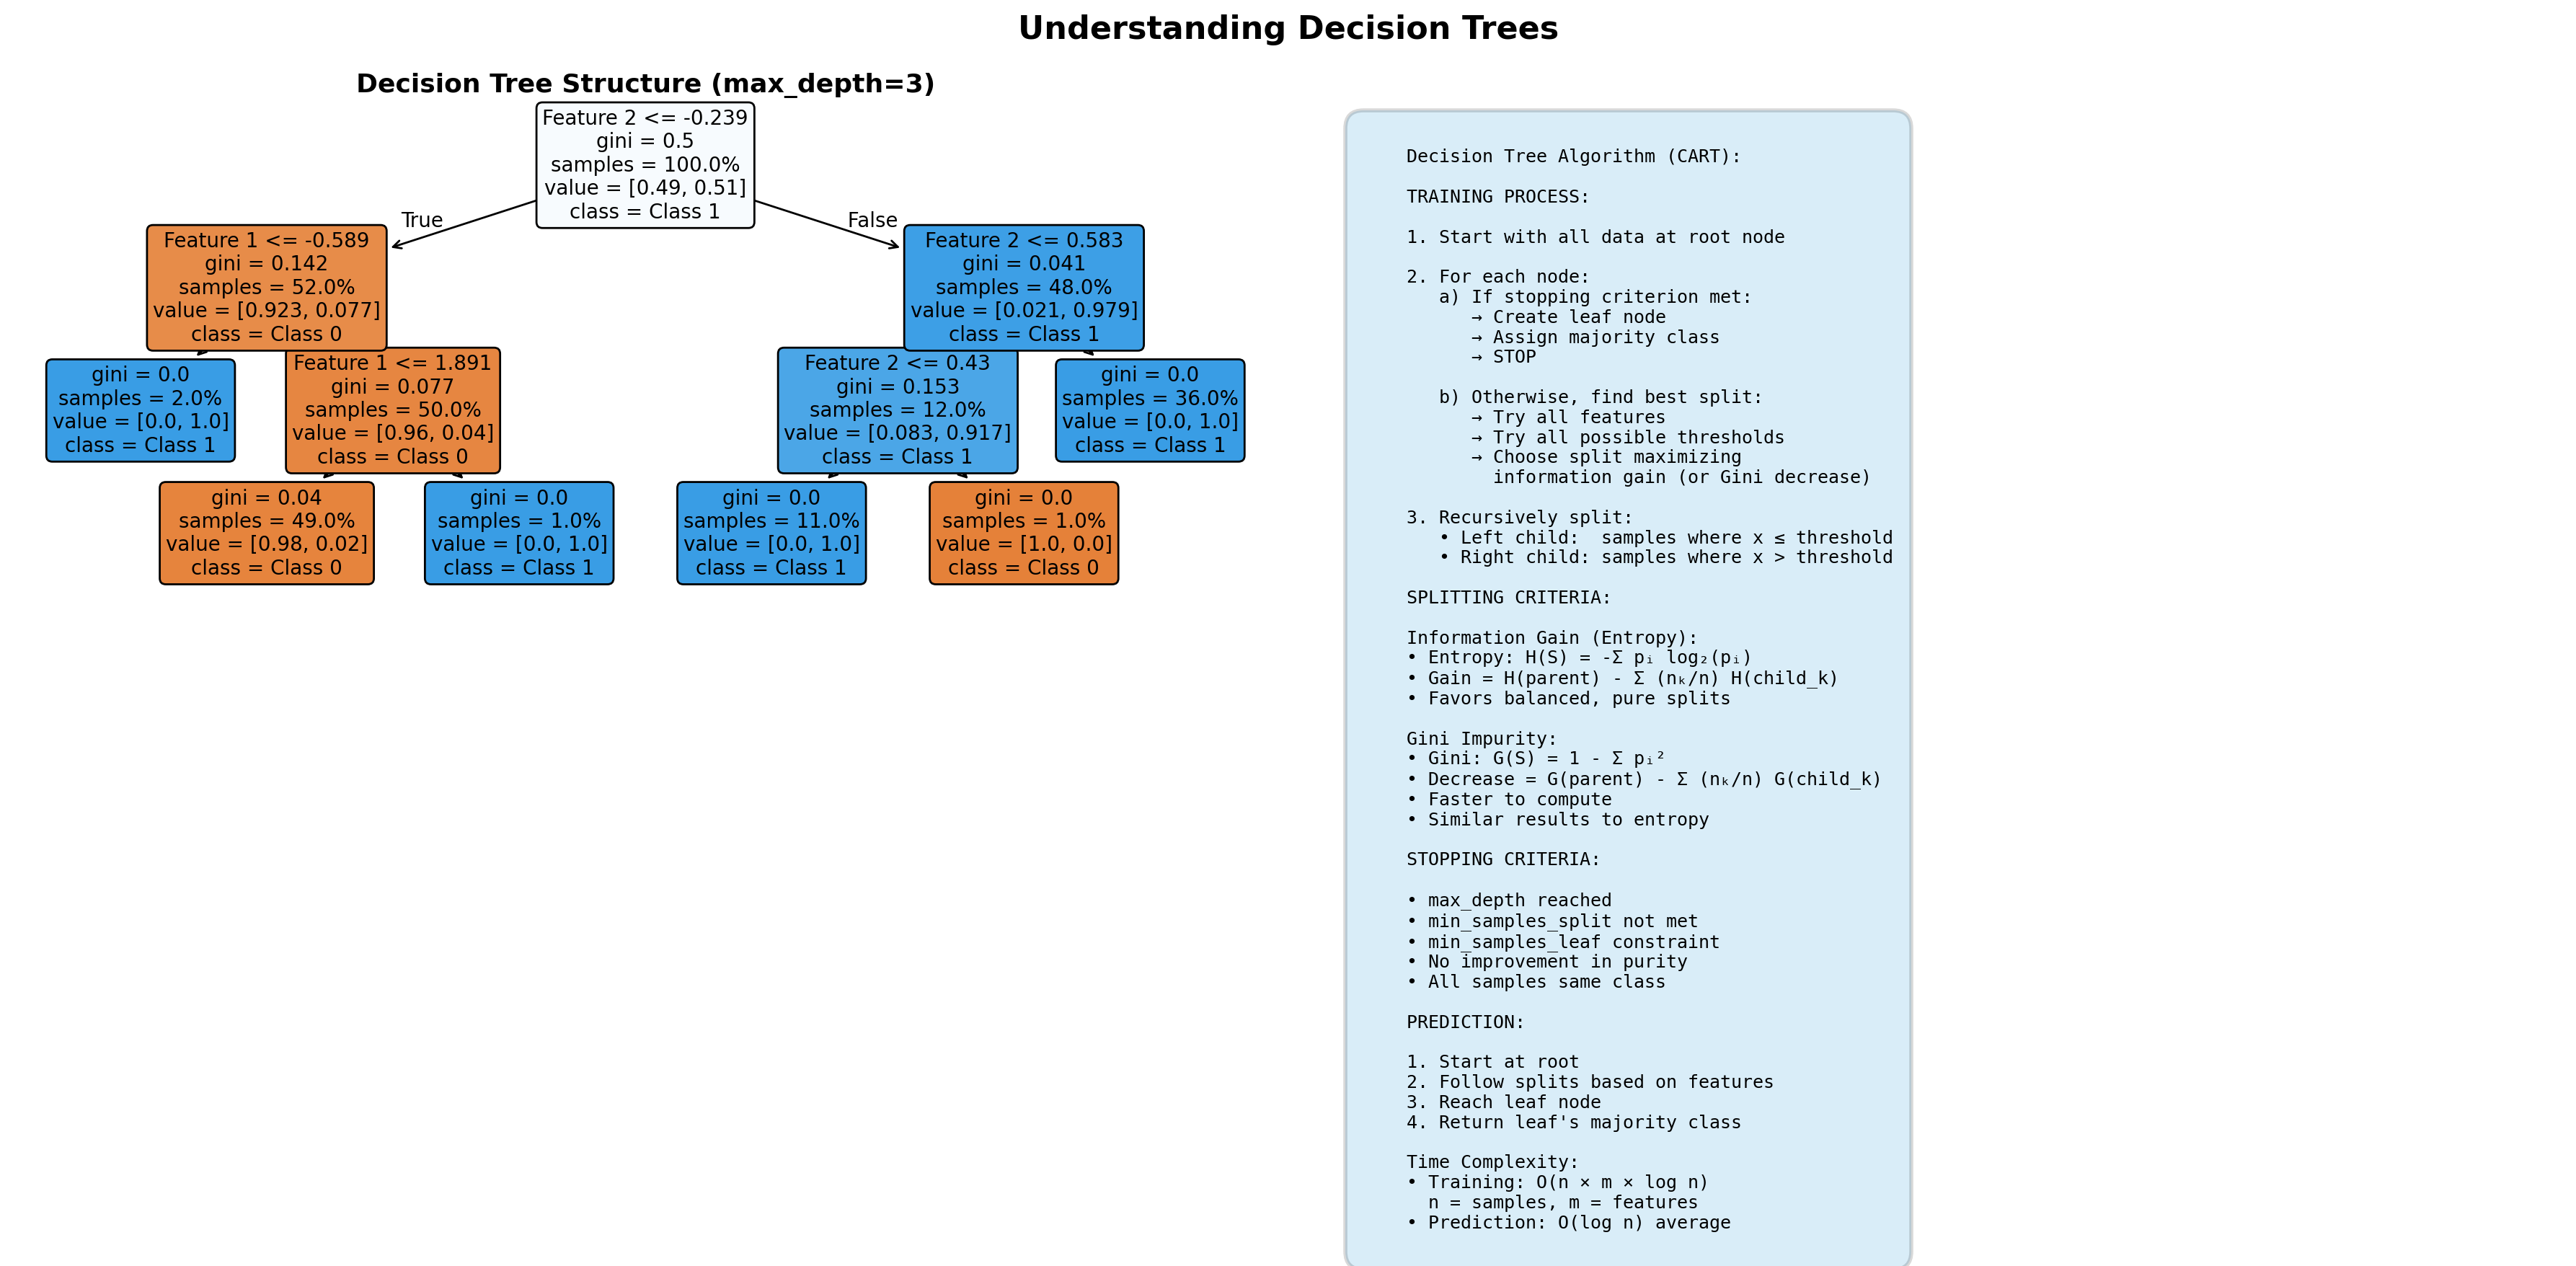
\includegraphics[width=\textwidth]{../figures/dt_tree_structure.png}
\end{column}
\end{columns}

\vspace{0.05cm}

\begin{alertblock}{Key Advantage}
Highly \textbf{interpretable} - can explain every decision!
\end{alertblock}
\end{frame}

\begin{frame}{Decision Tree: Example}

\textbf{Classification: Will a person buy a computer?}

\vspace{0.2cm}

\centering
\begin{tikzpicture}[
  level distance=1.8cm,
  level 1/.style={sibling distance=5cm},
  level 2/.style={sibling distance=2.5cm},
  every node/.style={rectangle, draw, rounded corners, align=center, minimum height=0.8cm},
  leaf/.style={rectangle, draw, fill=green!20, rounded corners},
  internal/.style={rectangle, draw, fill=blue!15, rounded corners}
]

\node[internal] {Age?}
  child {node[internal] {Student?}
    child {node[leaf] {Yes\\Buy}
      edge from parent node[left, draw=none] {Yes}}
    child {node[leaf] {No\\Don't Buy}
      edge from parent node[right, draw=none] {No}}
    edge from parent node[left, draw=none] {$\leq 30$}
  }
  child {node[leaf] {Yes\\Buy}
    edge from parent node[above, draw=none] {31-40}
  }
  child {node[internal] {Credit?}
    child {node[leaf] {Yes\\Buy}
      edge from parent node[left, draw=none] {Good}}
    child {node[leaf] {No\\Don't Buy}
      edge from parent node[right, draw=none] {Poor}}
    edge from parent node[right, draw=none] {$> 40$}
  };
\end{tikzpicture}

\vspace{0.3cm}

\begin{exampleblock}{Example Classification}
\textbf{Query:} Age=35, Student=No, Credit=Good

\textbf{Path:} Age $>$ 40? No $\rightarrow$ Age 31-40? Yes $\rightarrow$ \textcolor{green!60!black}{\textbf{Buy}}
\end{exampleblock}
\end{frame}

\begin{frame}{Building Decision Trees: CART Algorithm}

\begin{block}{CART = Classification And Regression Trees}
\textbf{Greedy recursive algorithm:}
\begin{enumerate}
\setlength{\itemsep}{3pt}
\item Start with all data at root
\item Find \textbf{best split} that maximizes information gain
\item Partition data into two subsets
\item Recursively build left and right subtrees
\item Stop when stopping criterion met (pure node, max depth, min samples)
\end{enumerate}
\end{block}

\vspace{0.15cm}

\begin{alertblock}{Key Question}
How do we determine the "\textbf{best split}"?

$\Rightarrow$ Use splitting criteria: Gini impurity or entropy
\end{alertblock}

\vspace{0.15cm}

\begin{exampleblock}{Splitting Decision}
For each feature $j$ and threshold $t$:
\begin{itemize}
\item Split data: $\mathcal{D}_{\text{left}} = \{\mathbf{x} | x_j \leq t\}$, $\mathcal{D}_{\text{right}} = \{\mathbf{x} | x_j > t\}$
\item Compute impurity of split
\item Choose $(j, t)$ with lowest impurity
\end{itemize}
\end{exampleblock}
\end{frame}

\begin{frame}{Splitting Criteria}

\begin{block}{1. Gini Impurity (CART default)}
Measures probability of incorrect classification:

$$\text{Gini}(D) = 1 - \sum_{k=1}^{C} p_k^2$$

where $p_k$ = proportion of class $k$ in dataset $D$

\vspace{0.05cm}

\textbf{Range:} [0, 1], where 0 = pure (all same class), higher = more mixed

\textbf{Interpretation:} Probability of misclassifying if label randomly assigned
\end{block}

\begin{block}{2. Entropy (ID3, C4.5 algorithms)}
Measures disorder/uncertainty:

$$\text{Entropy}(D) = -\sum_{k=1}^{C} p_k \log_2(p_k)$$

\textbf{Range:} [0, $\log_2 C$], where 0 = pure, higher = more uncertain

\textbf{Interpretation:} Average number of bits needed to encode class
\end{block}

\vspace{0.05cm}

\centering
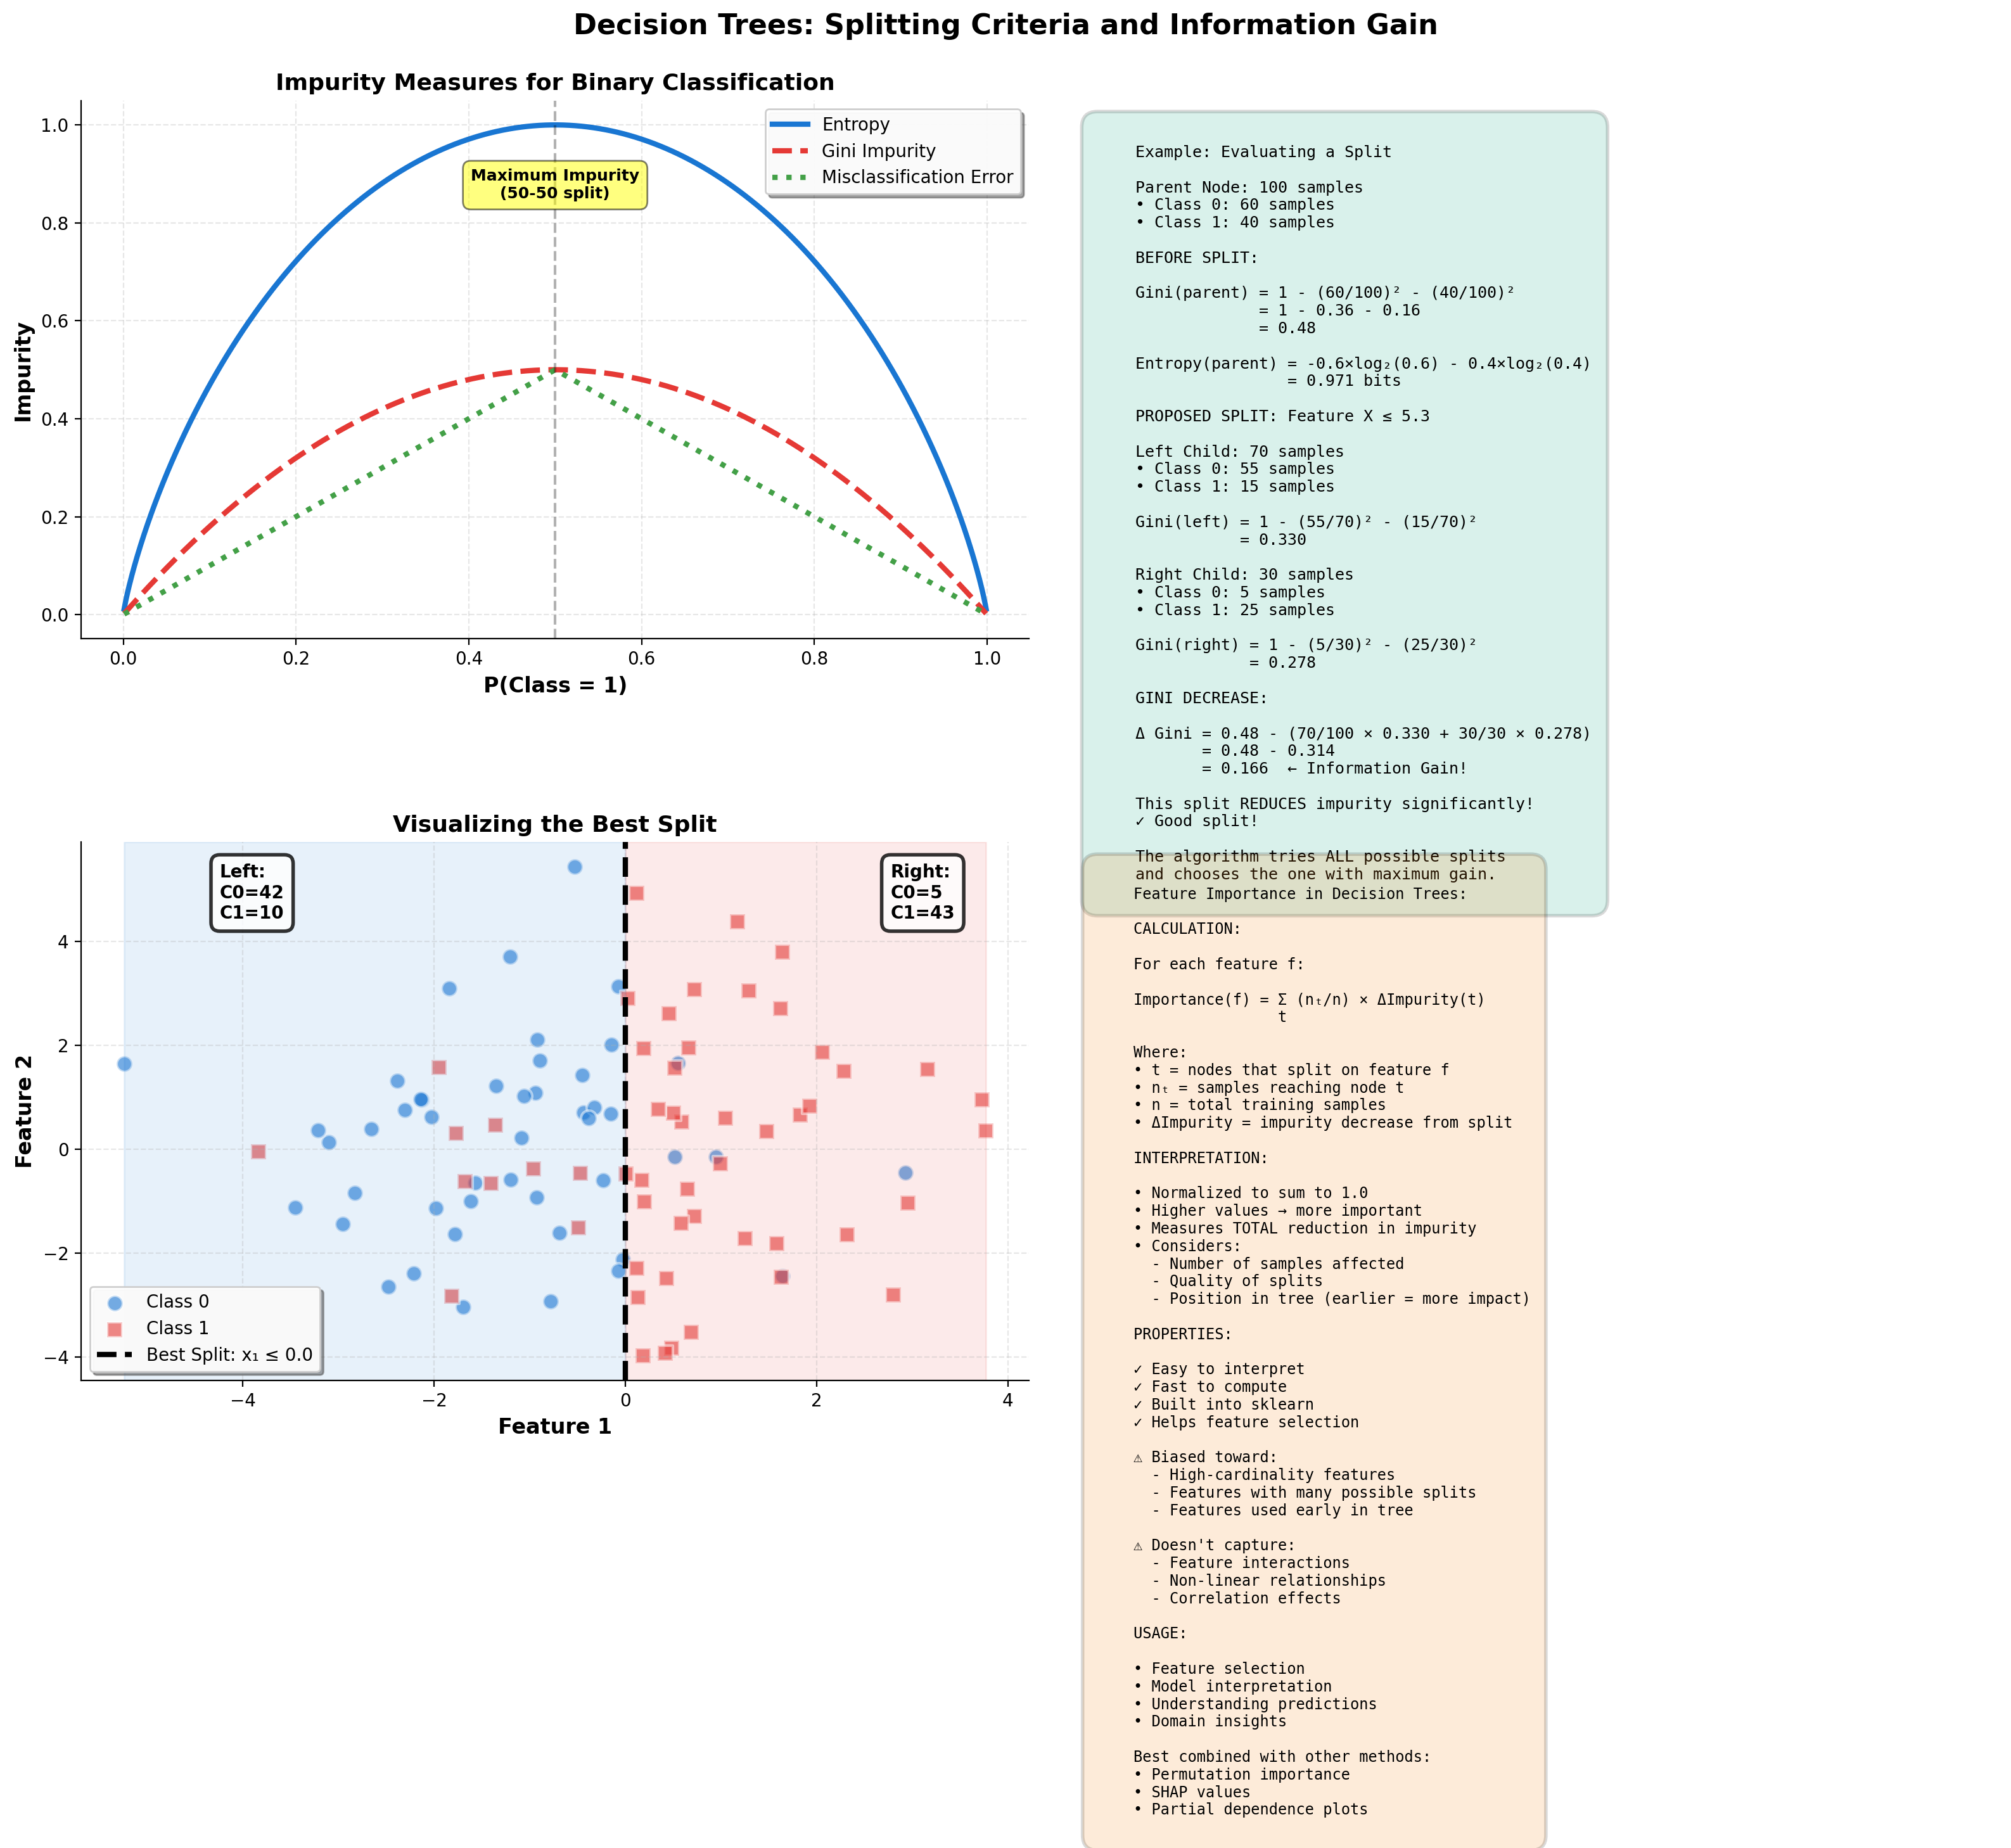
\includegraphics[width=0.65\textwidth]{../figures/dt_splitting_criteria.png}
\end{frame}

\begin{frame}{Information Gain}

\begin{block}{Definition}
\textbf{Information Gain} = Reduction in impurity after split

$$\text{IG}(D, j, t) = \text{Impurity}(D) - \left( \frac{|D_L|}{|D|} \text{Impurity}(D_L) + \frac{|D_R|}{|D|} \text{Impurity}(D_R) \right)$$

where:
\begin{itemize}
\item $D$ = parent dataset
\item $D_L$ = left child (samples with $x_j \leq t$)
\item $D_R$ = right child (samples with $x_j > t$)
\item $|D|$ = number of samples
\end{itemize}
\end{block}

\vspace{0.15cm}

\begin{exampleblock}{Splitting Algorithm}
\textbf{For each feature $j$ and each possible threshold $t$:}
\begin{enumerate}
\setlength{\itemsep}{2pt}
\item Compute information gain IG$(D, j, t)$
\item Keep track of best $(j^*, t^*)$ with highest gain
\end{enumerate}

\textbf{Split on} $(j^*, t^*)$ to maximize information gain
\end{exampleblock}

\vspace{0.05cm}

\begin{alertblock}{Goal}
Maximize purity of child nodes (minimize impurity)
\end{alertblock}
\end{frame}

\begin{frame}{Decision Tree Example: Manual Construction}

\textbf{Dataset: Play tennis? (same as Naive Bayes example)}

\vspace{0.1cm}

\begin{columns}[T]
\begin{column}{0.42\textwidth}
\begin{block}{Training Data (9 samples)}
\tiny
\begin{tabular}{cccc}
\toprule
Outlook & Temp & Humidity & Play \\
\midrule
Sunny & Hot & High & No \\
Sunny & Hot & High & No \\
Overcast & Hot & High & Yes \\
Rainy & Mild & High & Yes \\
Rainy & Cool & Normal & Yes \\
Rainy & Cool & Normal & No \\
Overcast & Cool & Normal & Yes \\
Sunny & Mild & High & No \\
Sunny & Cool & Normal & Yes \\
\bottomrule
\end{tabular}
\end{block}

\vspace{0.05cm}

\begin{exampleblock}{Class Distribution}
Yes: 5, No: 4
\end{exampleblock}
\end{column}

\begin{column}{0.56\textwidth}
\begin{block}{Step 1: Compute Root Entropy}
\small
$$\text{Entropy}(\text{root}) = -\frac{5}{9}\log_2\frac{5}{9} - \frac{4}{9}\log_2\frac{4}{9}$$
$$\approx 0.994 \text{ bits}$$
\end{block}

\begin{block}{Step 2: Try Splitting on Outlook}
\small
\textbf{Sunny} (3 samples): No=2, Yes=1\\
$\text{Entropy} = -\frac{2}{3}\log_2\frac{2}{3} - \frac{1}{3}\log_2\frac{1}{3} \approx 0.918$

\textbf{Overcast} (2 samples): Yes=2\\
$\text{Entropy} = 0$ (pure!)

\textbf{Rainy} (4 samples): Yes=2, No=1, Yes=1\\
$\text{Entropy} = -\frac{2}{4}\log_2\frac{2}{4} - \frac{2}{4}\log_2\frac{2}{4} = 1.0$
\end{block}

\begin{block}{Step 3: Information Gain}
\small
$$\text{IG}(\text{Outlook}) = 0.994 - \left(\frac{3}{9}(0.918) + \frac{2}{9}(0) + \frac{4}{9}(1.0)\right)$$
$$= 0.994 - 0.750 = \mathbf{0.244}$$

\textbf{Result:} Outlook has good information gain!
\end{block}
\end{column}
\end{columns}
\end{frame}

\begin{frame}{Decision Tree: Iris Dataset Example}

\centering
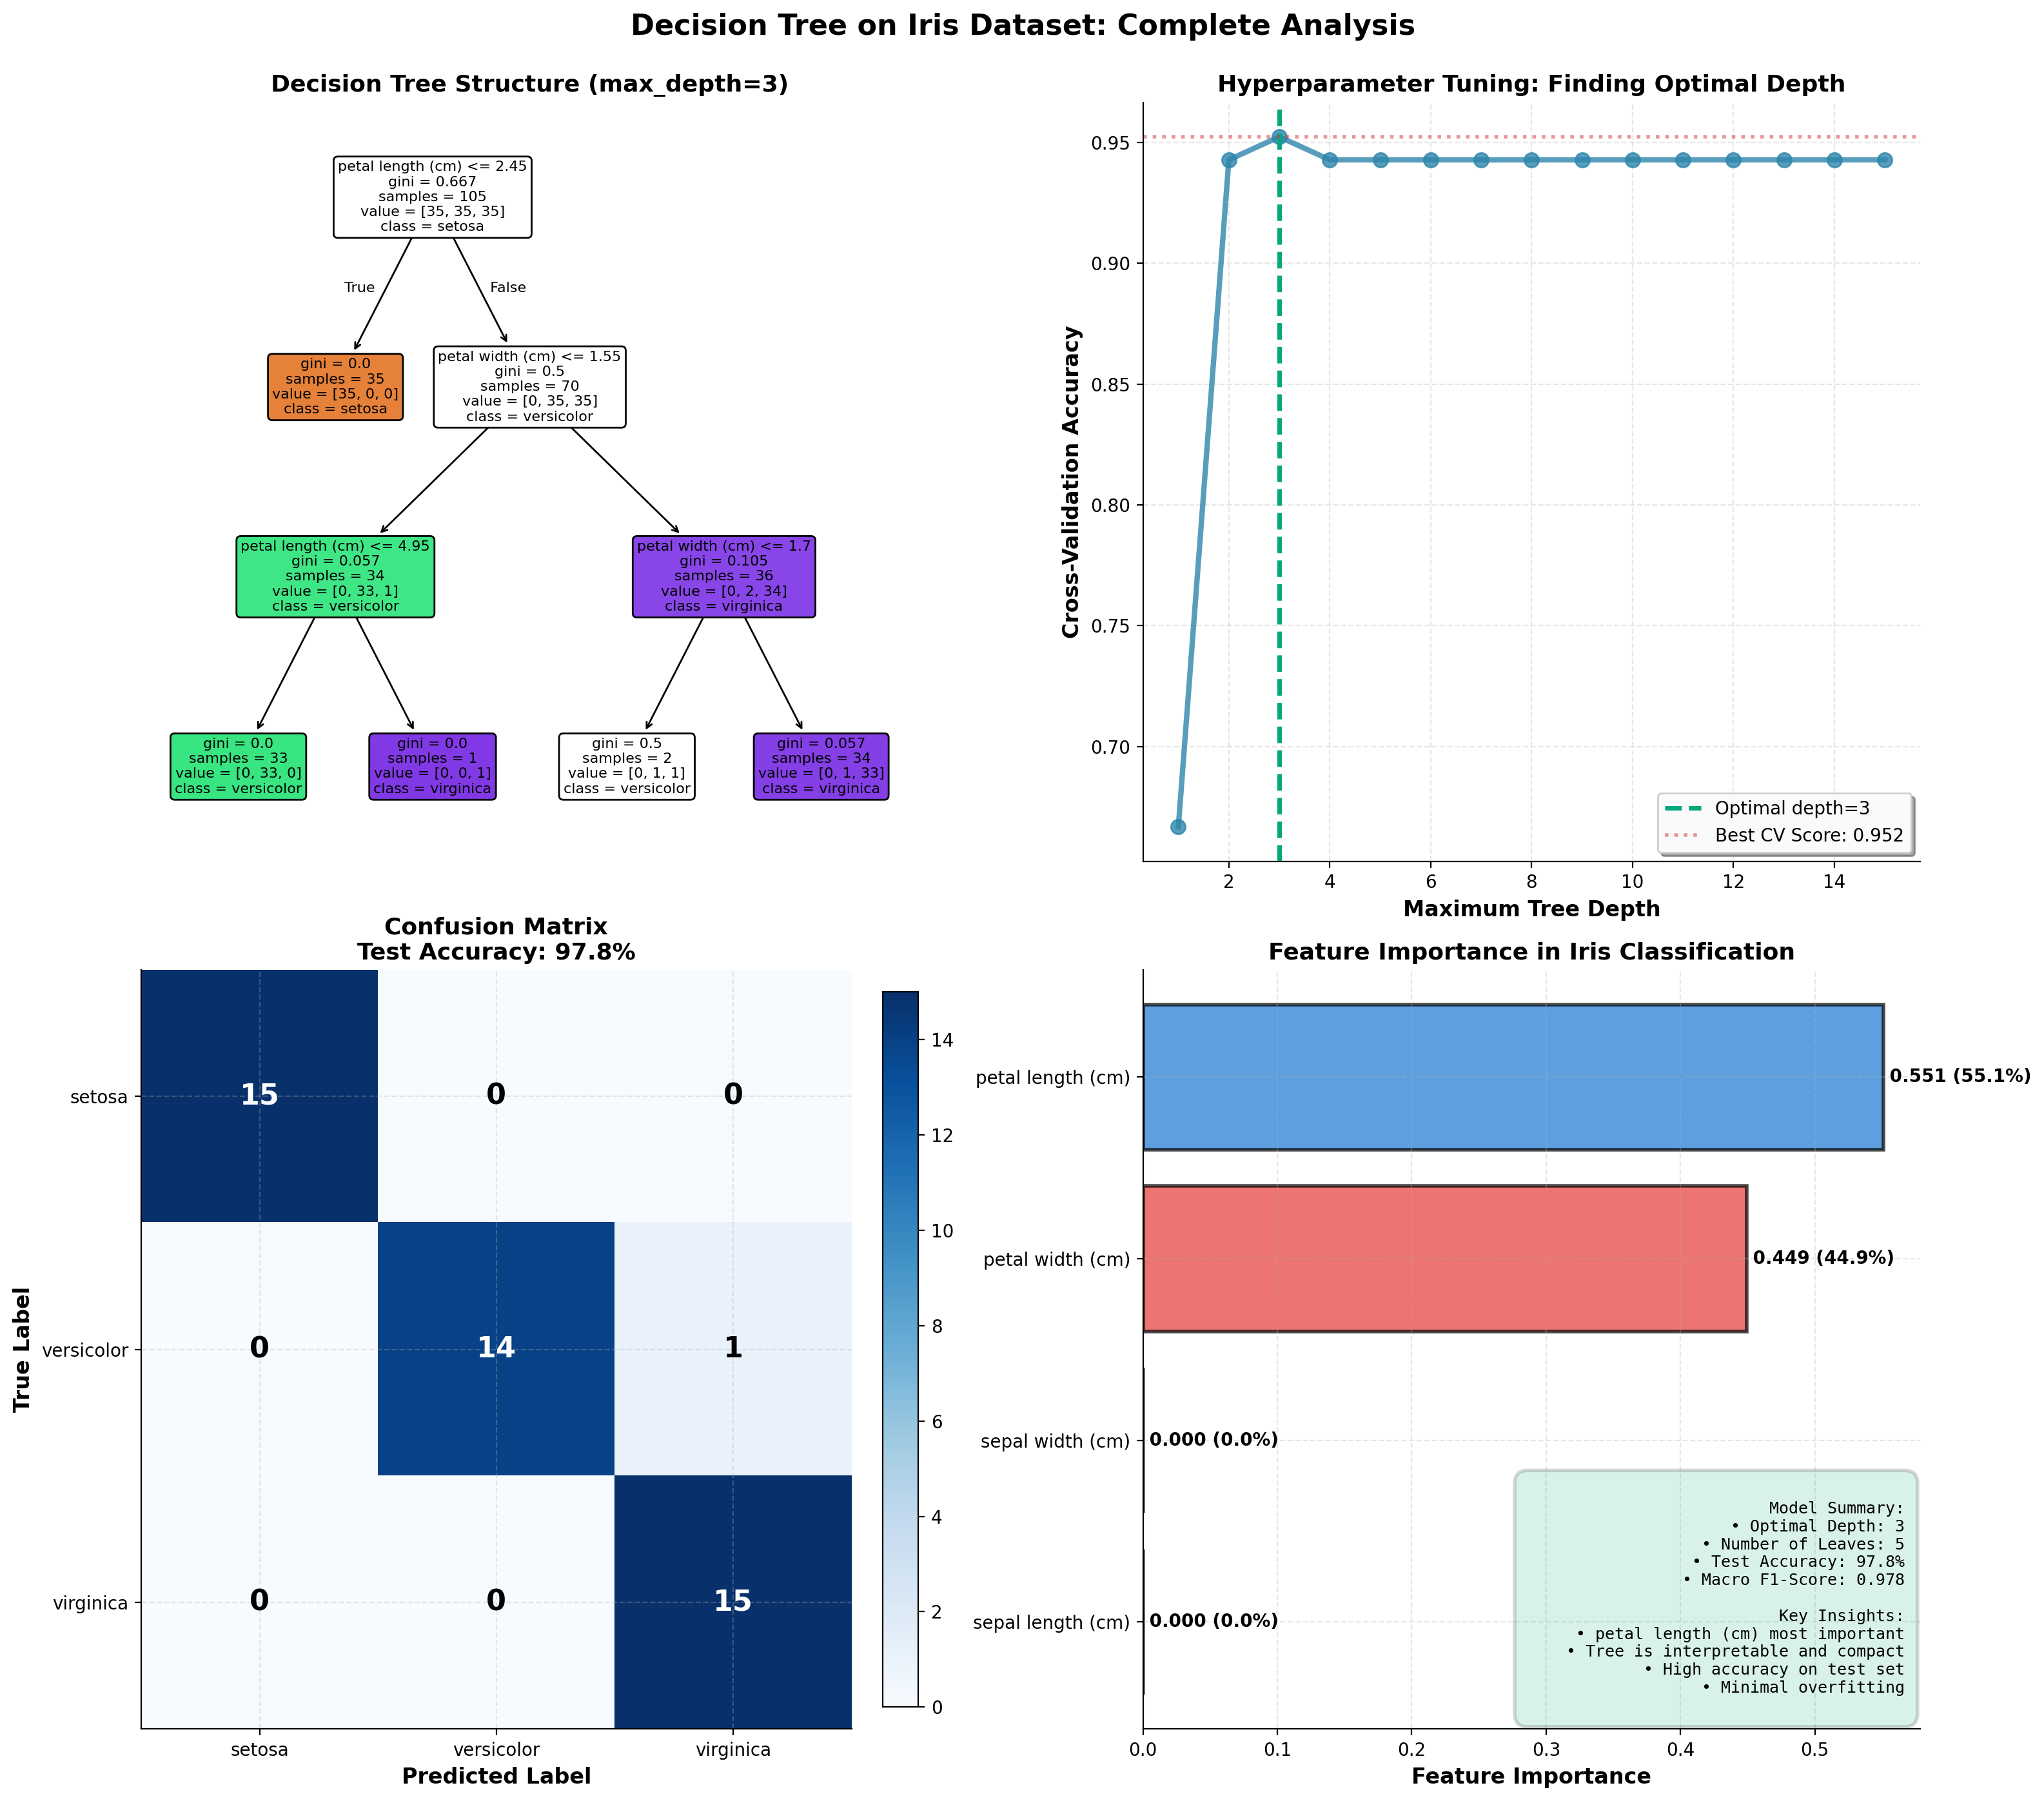
\includegraphics[width=0.92\textwidth]{../figures/dt_iris_example.png}

\vspace{0.05cm}

\begin{columns}[T]
\begin{column}{0.48\textwidth}
\begin{exampleblock}{Performance (max\_depth=3)}
\begin{itemize}
\setlength{\itemsep}{1pt}
\item \textbf{Training Accuracy:} 98.3\%
\item \textbf{Test Accuracy:} 93.3\%
\item \textbf{Tree Depth:} 3
\item \textbf{Number of Leaves:} 5
\end{itemize}
\end{exampleblock}
\end{column}

\begin{column}{0.48\textwidth}
\begin{alertblock}{Key Observations}
\begin{itemize}
\setlength{\itemsep}{1pt}
\item Axis-aligned decision boundaries
\item Interpretable rules
\item Feature importance clear
\item Some overfitting without pruning
\end{itemize}
\end{alertblock}
\end{column}
\end{columns}
\end{frame}

\begin{frame}{Decision Boundaries: Different Depths}

\centering
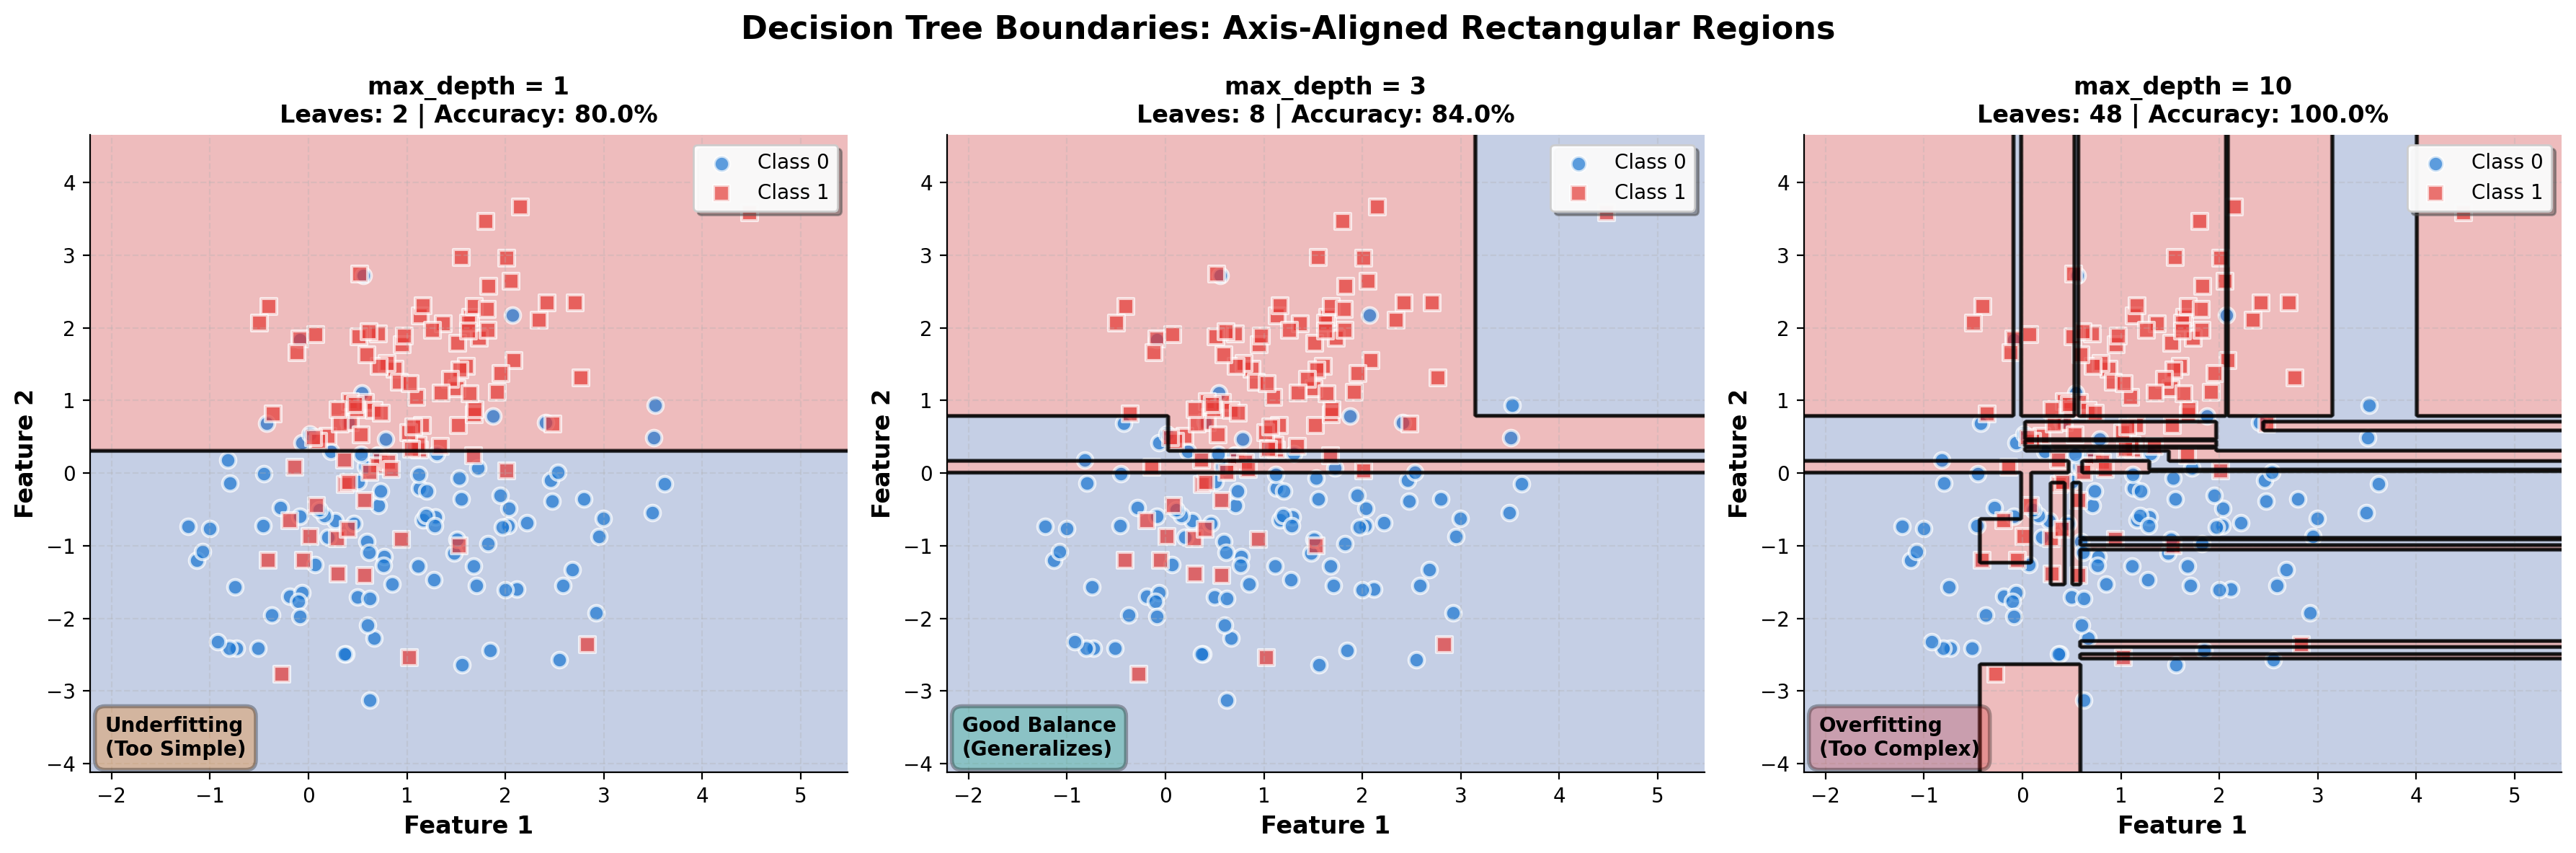
\includegraphics[width=0.95\textwidth]{../figures/dt_decision_boundaries.png}

\vspace{0.05cm}

\begin{columns}[T]
\begin{column}{0.32\textwidth}
\begin{block}{Depth = 2}
\begin{itemize}
\setlength{\itemsep}{0pt}
\item Simple boundaries
\item High bias
\item Underfits
\end{itemize}
\end{block}
\end{column}

\begin{column}{0.32\textwidth}
\begin{block}{Depth = 5}
\begin{itemize}
\setlength{\itemsep}{0pt}
\item Balanced
\item Good generalization
\item Optimal complexity
\end{itemize}
\end{block}
\end{column}

\begin{column}{0.32\textwidth}
\begin{block}{Depth = 20}
\begin{itemize}
\setlength{\itemsep}{0pt}
\item Complex boundaries
\item High variance
\item Overfits
\end{itemize}
\end{block}
\end{column}
\end{columns}

\vspace{0.05cm}

\begin{alertblock}{Key Insight}
Decision trees create \textbf{axis-aligned rectangular} decision regions!
\end{alertblock}
\end{frame}

\begin{frame}[fragile]{Decision Tree Algorithm (Pseudocode)}

\begin{algorithm}[H]
\caption{CART Decision Tree (Recursive)}
\begin{algorithmic}[1]
\REQUIRE Dataset $D$, features $F$, max\_depth, min\_samples
\ENSURE Decision tree $T$

\STATE \textbf{function} BuildTree($D$, depth)
\IF{stopping criterion met}
    \STATE \textbf{return} LeafNode(majority class in $D$)
\ENDIF

\STATE $\text{best\_gain} \gets 0$
\STATE $(j^*, t^*) \gets \text{None}$

\FOR{each feature $j \in F$}
    \FOR{each threshold $t$ (midpoints of sorted values)}
        \STATE Split: $D_L \gets \{\mathbf{x} \in D : x_j \leq t\}$, $D_R \gets \{\mathbf{x} \in D : x_j > t\}$
        \STATE $\text{gain} \gets \text{InformationGain}(D, D_L, D_R)$
        \IF{gain $>$ best\_gain}
            \STATE $\text{best\_gain} \gets \text{gain}$
            \STATE $(j^*, t^*) \gets (j, t)$
        \ENDIF
    \ENDFOR
\ENDFOR

\STATE $D_L, D_R \gets$ Split $D$ on feature $j^*$ at threshold $t^*$
\STATE $T_L \gets$ BuildTree($D_L$, depth + 1)
\STATE $T_R \gets$ BuildTree($D_R$, depth + 1)
\STATE \textbf{return} DecisionNode($j^*, t^*, T_L, T_R$)
\end{algorithmic}
\end{algorithm}
\end{frame}

\begin{frame}{Overfitting and Pruning}

\centering
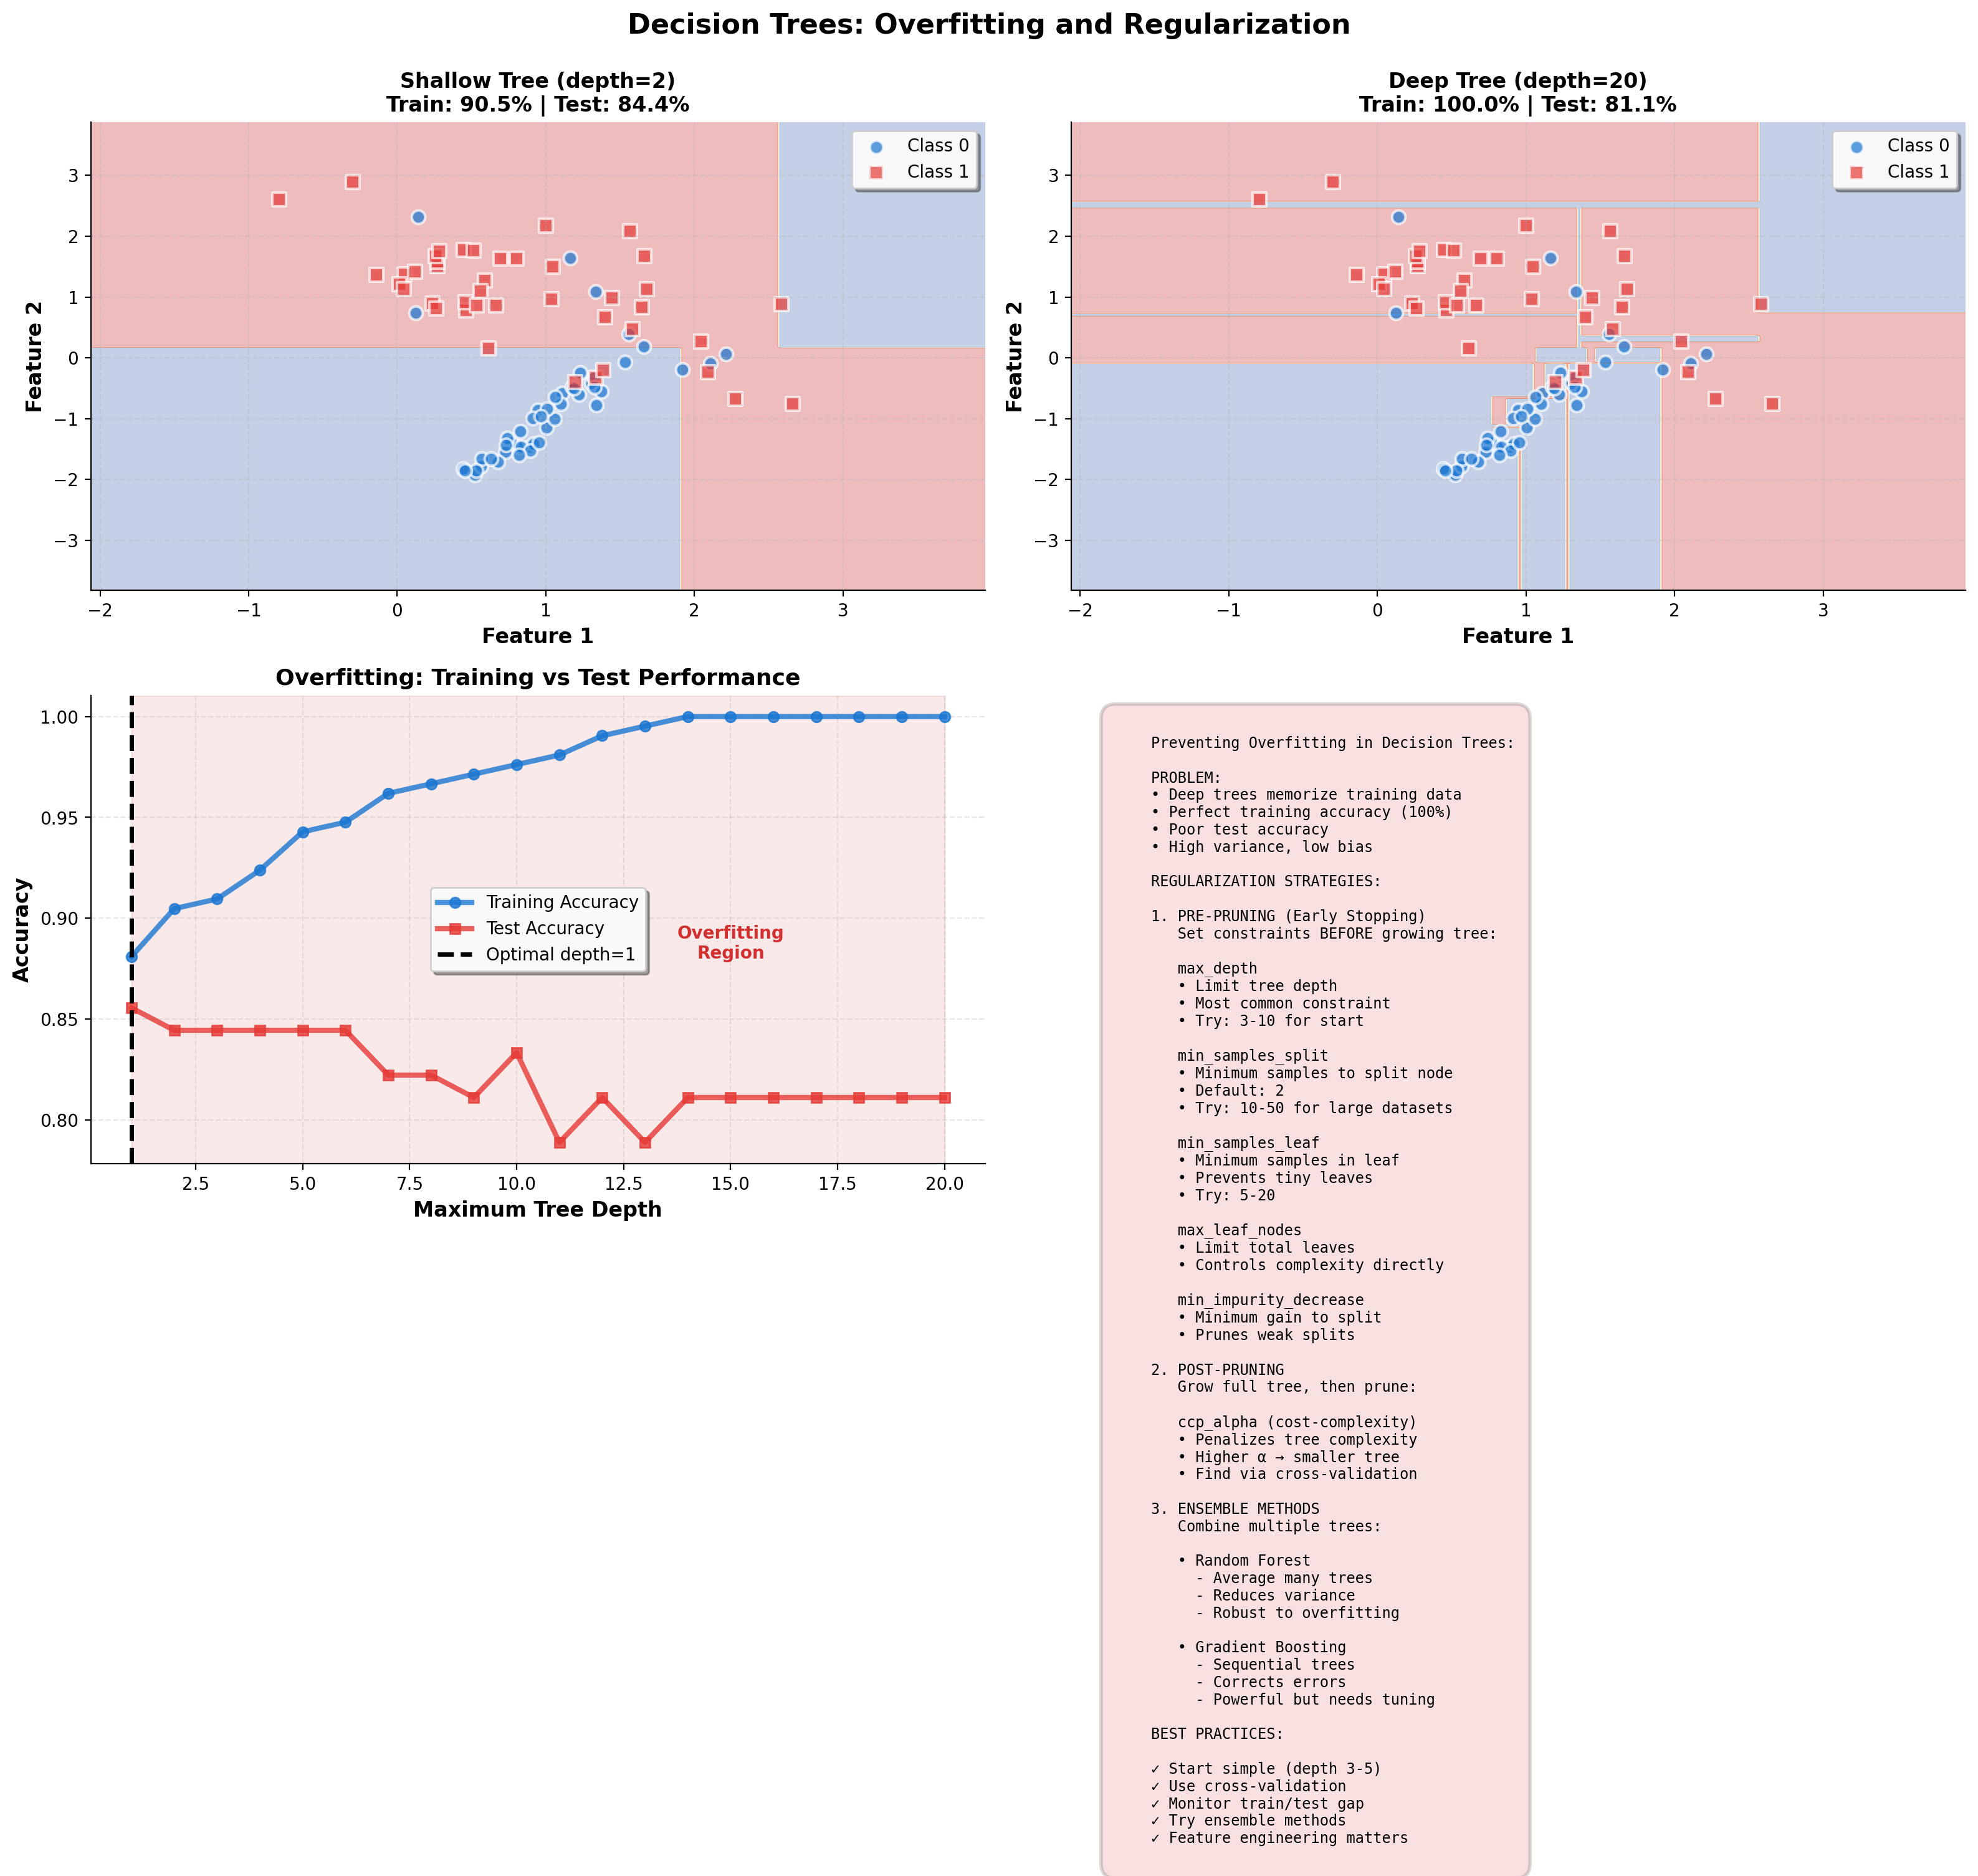
\includegraphics[width=0.85\textwidth]{../figures/dt_overfitting.png}

\vspace{0.1cm}

\begin{columns}[t]
\begin{column}{0.48\textwidth}
\begin{alertblock}{Overfitting Problem}
\begin{itemize}
\setlength{\itemsep}{2pt}
\item Deep trees memorize training data
\item Poor generalization
\item High variance
\item Noisy patterns captured
\end{itemize}
\end{alertblock}

\vspace{0.1cm}

\begin{block}{Pre-Pruning (Early Stopping)}
Stop growing tree when:
\begin{itemize}
\setlength{\itemsep}{1pt}
\item Max depth reached
\item Min samples per node
\item Min information gain
\item Max number of leaves
\end{itemize}
\end{block}
\end{column}

\begin{column}{0.48\textwidth}
\begin{block}{Post-Pruning}
\begin{itemize}
\setlength{\itemsep}{2pt}
\item Grow full tree first
\item Remove subtrees that don't improve validation accuracy
\item Use cost-complexity pruning
\item More expensive but often better
\end{itemize}
\end{block}

\vspace{0.1cm}

\begin{exampleblock}{Best Practice}
\begin{itemize}
\setlength{\itemsep}{2pt}
\item Use cross-validation to tune parameters
\item Start with max\_depth $\in [3, 10]$
\item Require min\_samples\_split $\geq 20$
\item Monitor train vs validation accuracy
\end{itemize}
\end{exampleblock}
\end{column}
\end{columns}
\end{frame}

\begin{frame}{Feature Importance}

\begin{columns}[t]
\begin{column}{0.52\textwidth}
\begin{block}{Computing Importance}
For each feature $j$:

$$\text{Importance}(j) = \sum_{\text{nodes using } j} \frac{n_{\text{node}}}{n_{\text{total}}} \cdot \Delta\text{Impurity}$$

where:
\begin{itemize}
\item Sum over all nodes that split on feature $j$
\item Weight by fraction of samples at node
\item $\Delta\text{Impurity}$ = reduction in impurity
\end{itemize}
\end{block}

\vspace{0.1cm}

\begin{exampleblock}{Interpretation}
\begin{itemize}
\setlength{\itemsep}{2pt}
\item Higher importance = more useful for prediction
\item Normalized to sum to 1.0
\item Features not used have 0 importance
\item Can identify redundant features
\end{itemize}
\end{exampleblock}
\end{column}

\begin{column}{0.45\textwidth}
\centering
\vspace{0pt}
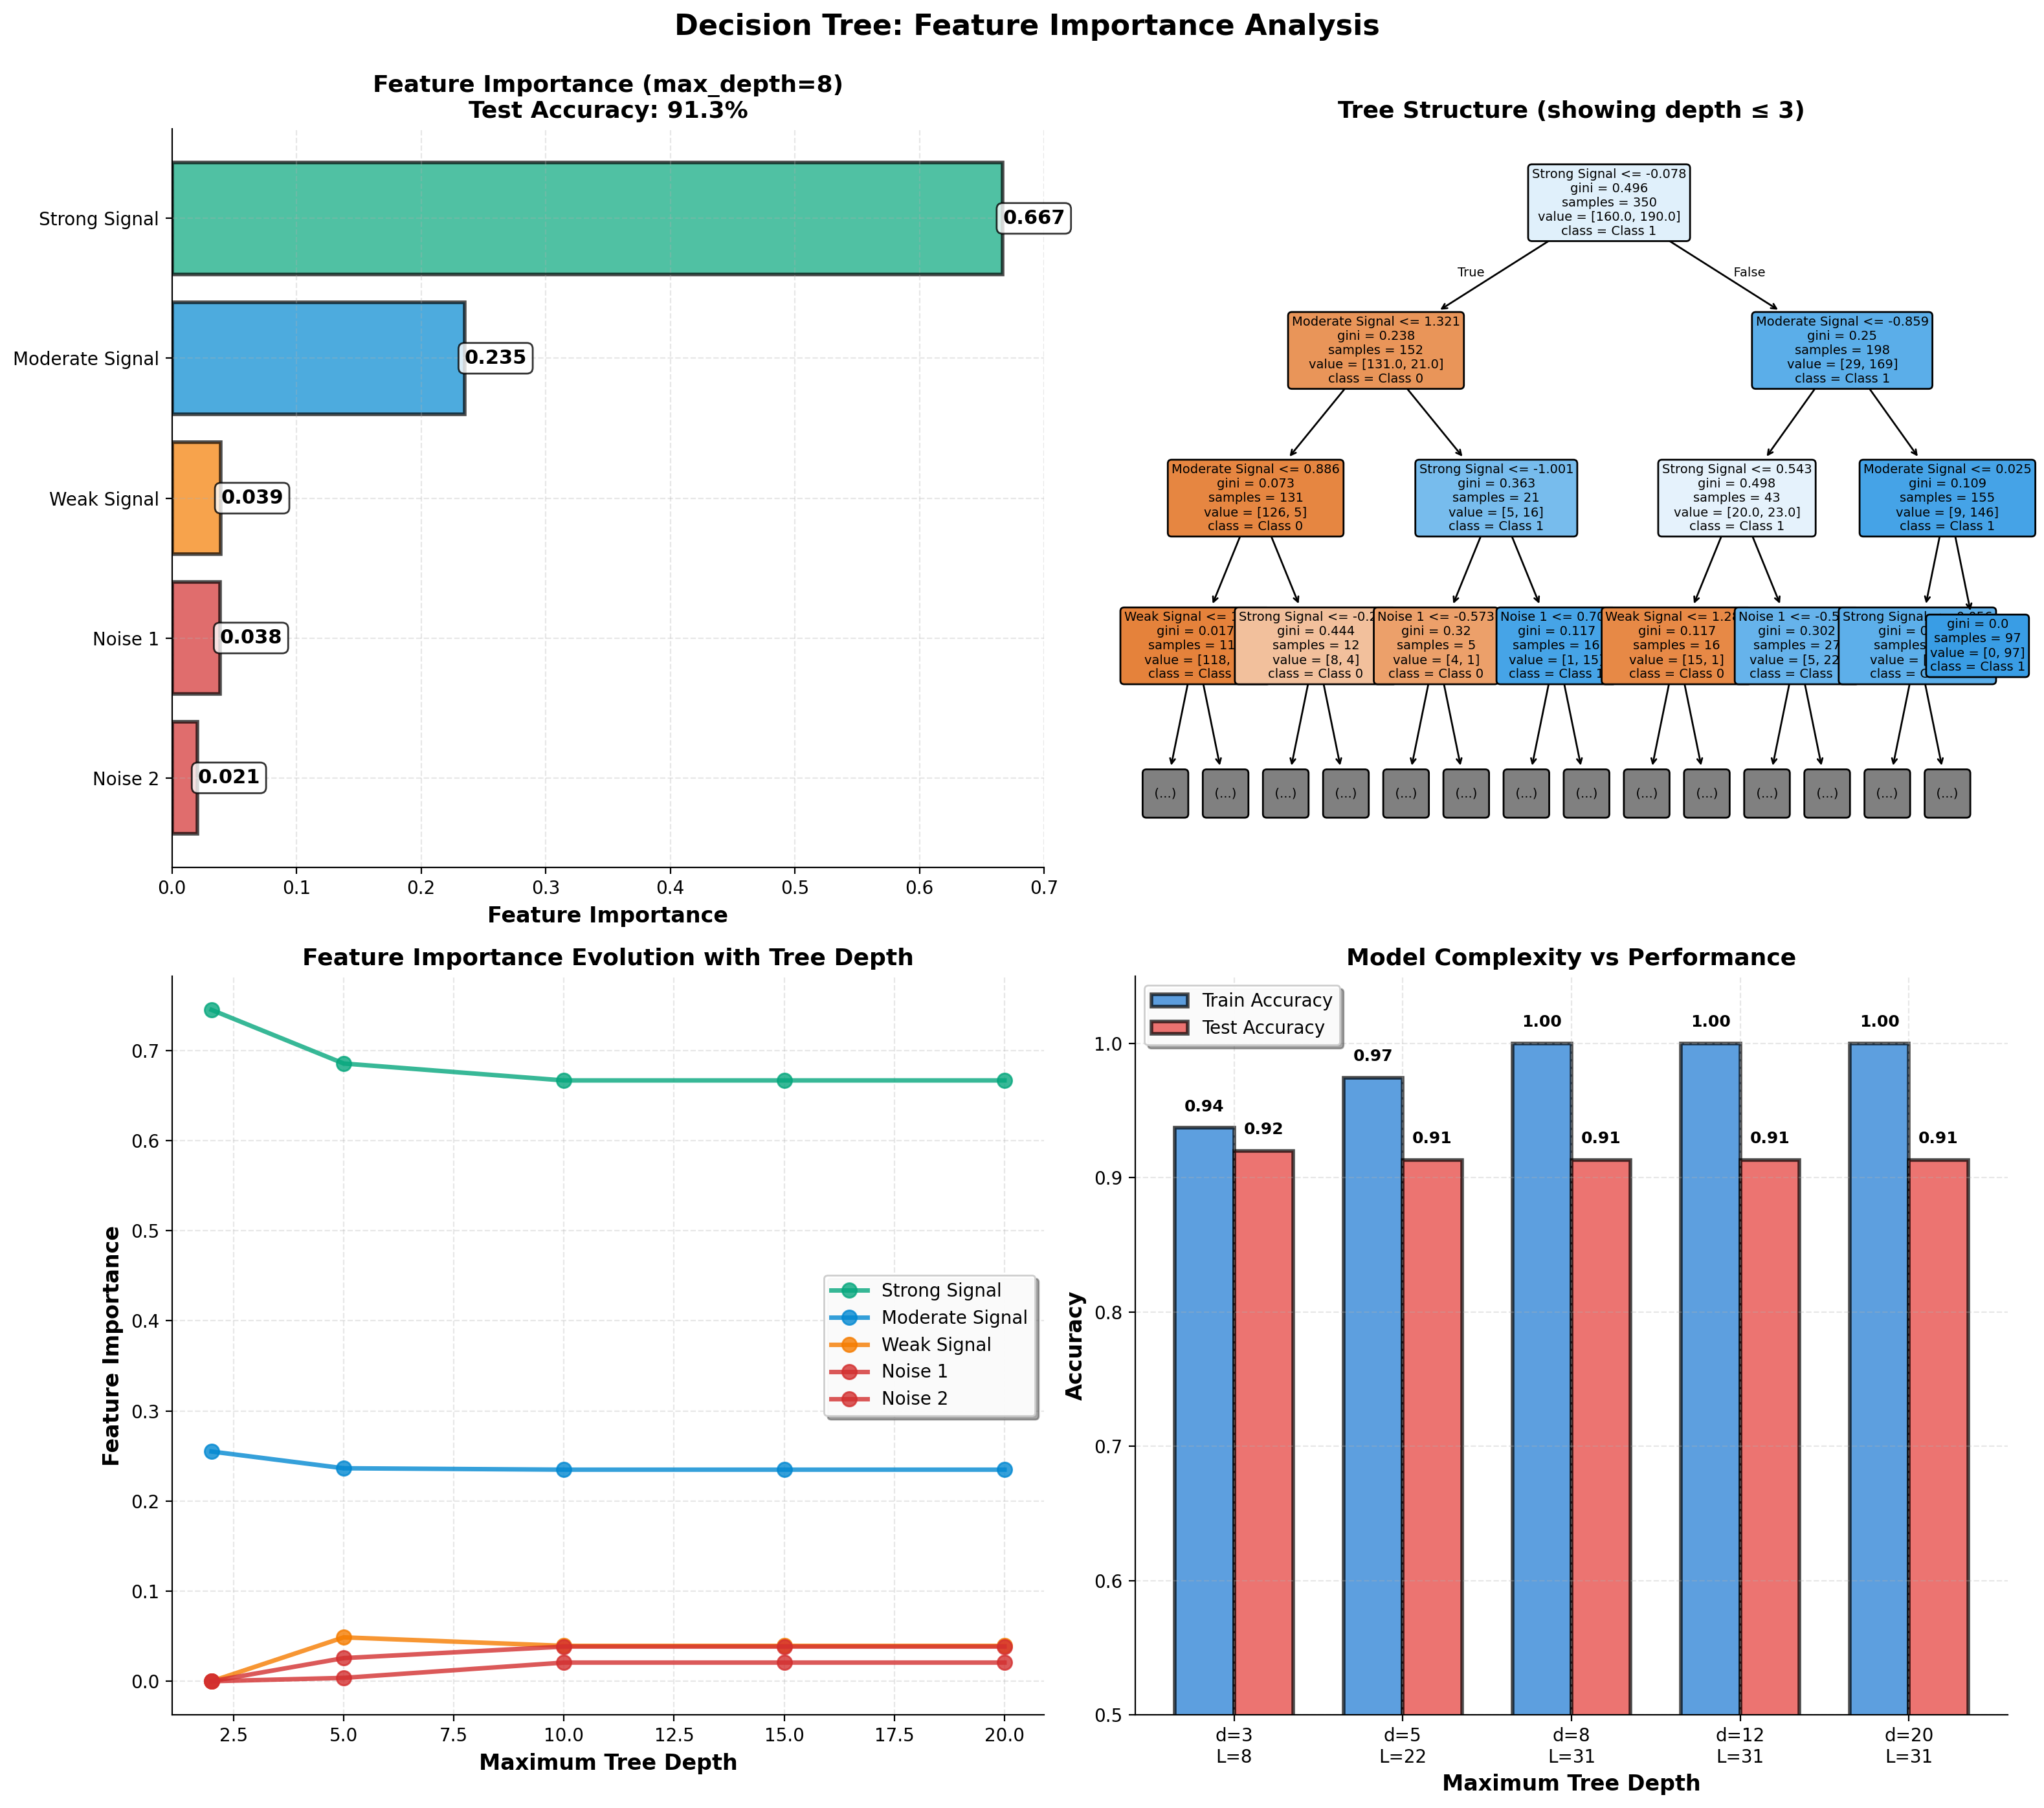
\includegraphics[width=\textwidth]{../figures/dt_feature_importance.png}
\end{column}
\end{columns}

\vspace{0.05cm}

\begin{alertblock}{Use Cases}
Feature selection, domain insights, model interpretation, debugging
\end{alertblock}
\end{frame}

\begin{frame}{Ensemble Methods Preview}

\begin{block}{Limitation: Single Tree Instability}
\begin{itemize}
\setlength{\itemsep}{2pt}
\item Small changes in data $\rightarrow$ very different tree
\item High variance
\item Sensitive to training set
\end{itemize}
\end{block}

\vspace{0.15cm}

\begin{exampleblock}{Solution: Ensemble Methods}
Combine multiple trees for better performance:

\vspace{0.1cm}

\textbf{1. Random Forest}
\begin{itemize}
\setlength{\itemsep}{1pt}
\item Train many trees on bootstrap samples
\item Random feature subset at each split
\item Average predictions (voting for classification)
\end{itemize}

\vspace{0.1cm}

\textbf{2. Gradient Boosting (XGBoost, LightGBM)}
\begin{itemize}
\setlength{\itemsep}{1pt}
\item Train trees sequentially
\item Each tree corrects errors of previous
\item Weighted combination of predictions
\end{itemize}

\vspace{0.1cm}

\textbf{3. AdaBoost}
\begin{itemize}
\setlength{\itemsep}{1pt}
\item Weighted training samples
\item Focus on hard-to-classify examples
\item Weighted voting
\end{itemize}
\end{exampleblock}

\vspace{0.05cm}

\begin{alertblock}{Note}
These methods will be covered in detail in the Ensemble Learning module!
\end{alertblock}
\end{frame}

\begin{frame}{Decision Trees: Advantages \& Disadvantages}

\begin{columns}[t]
\begin{column}{0.48\textwidth}
\begin{block}{Advantages}
\begin{itemize}
\setlength{\itemsep}{3pt}
\item \textbf{Interpretable:} Easy to visualize and explain
\item \textbf{No scaling:} Works with raw features
\item \textbf{Mixed types:} Handles numerical and categorical
\item \textbf{Non-linear:} Captures complex patterns
\item \textbf{Feature selection:} Automatic importance ranking
\item \textbf{Missing values:} Can handle with surrogates
\item \textbf{Fast prediction:} $O(\log n)$ time
\end{itemize}
\end{block}
\end{column}

\begin{column}{0.48\textwidth}
\begin{block}{Disadvantages}
\begin{itemize}
\setlength{\itemsep}{3pt}
\item \textbf{Overfitting:} Prone to high variance
\item \textbf{Instability:} Small data changes = big tree changes
\item \textbf{Axis-aligned:} Cannot capture diagonal boundaries well
\item \textbf{Biased:} Favors features with many values
\item \textbf{Imbalanced:} Struggles with skewed classes
\item \textbf{Local optima:} Greedy algorithm
\item \textbf{Extrapolation:} Poor outside training range
\end{itemize}
\end{block}
\end{column}
\end{columns}

\vspace{0.15cm}

\begin{alertblock}{When to Use Decision Trees}
\textbf{Good for:} Interpretability needed, mixed feature types, feature interactions, baseline model\\
\textbf{Avoid when:} Need best accuracy (use ensembles), many irrelevant features
\end{alertblock}
\end{frame}

% ========================================
% Section: Comparison
% ========================================

\section{Method Comparison \& Selection}

\begin{frame}{Comparison: Decision Boundaries}

\textbf{Visual comparison on synthetic 2D dataset:}

\vspace{0.2cm}

\begin{columns}[T]
\begin{column}{0.32\textwidth}
\centering
\textbf{Naive Bayes}
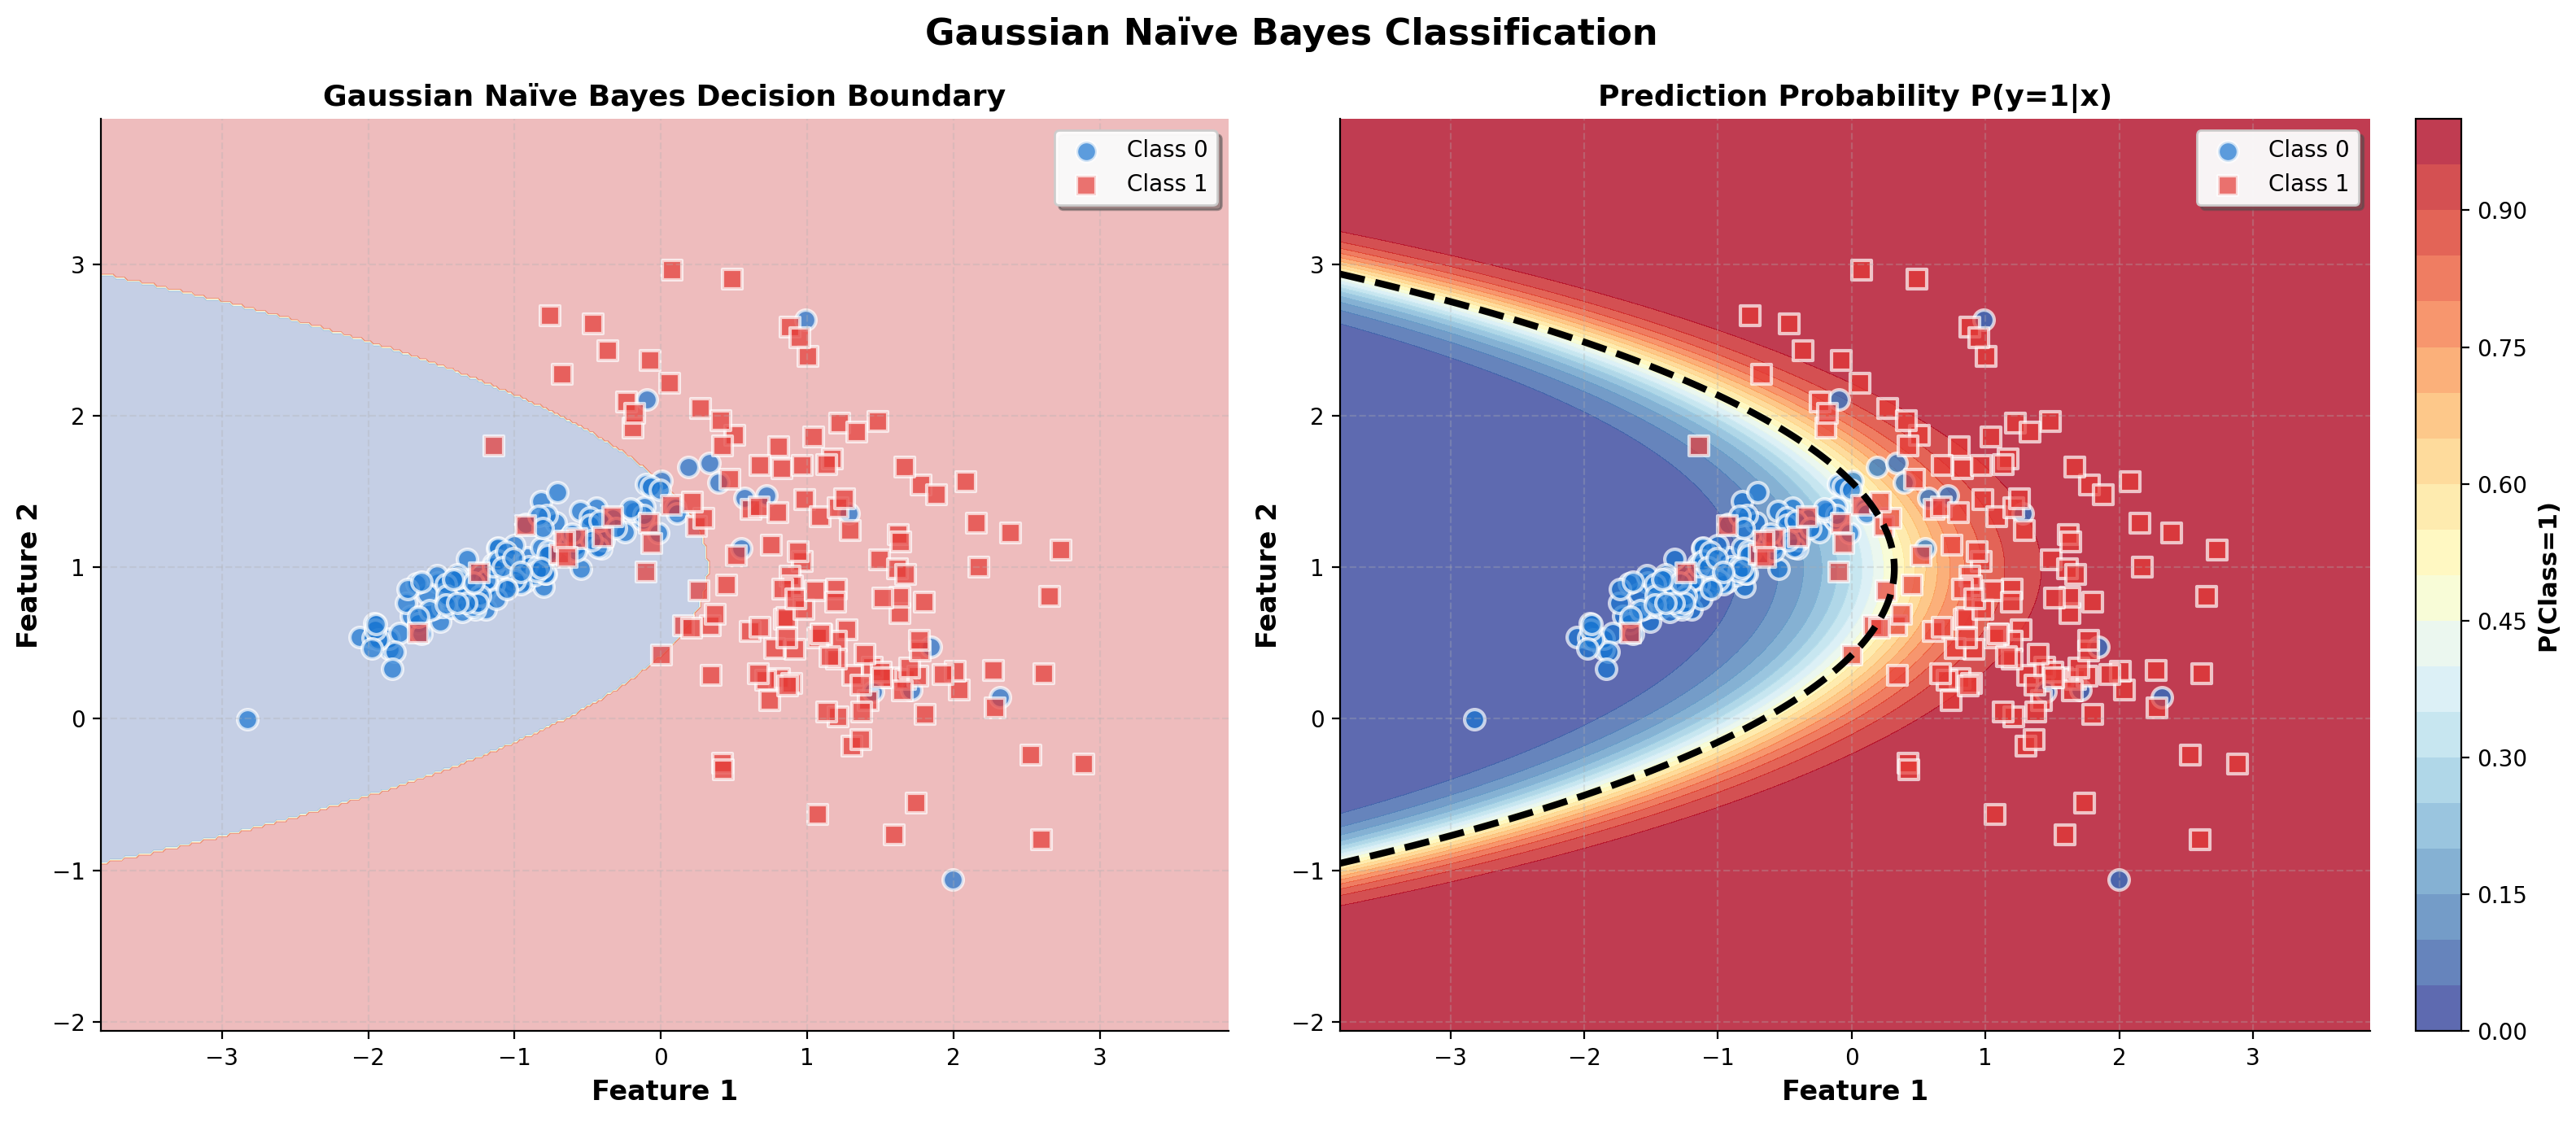
\includegraphics[width=\textwidth]{../figures/nb_gaussian_decision.png}

\begin{block}{\small Properties}
\begin{itemize}
\setlength{\itemsep}{0pt}
\small
\item Linear/quadratic
\item Smooth probabilistic
\item Assumes Gaussian
\end{itemize}
\end{block}
\end{column}

\begin{column}{0.32\textwidth}
\centering
\textbf{K-Nearest Neighbors}
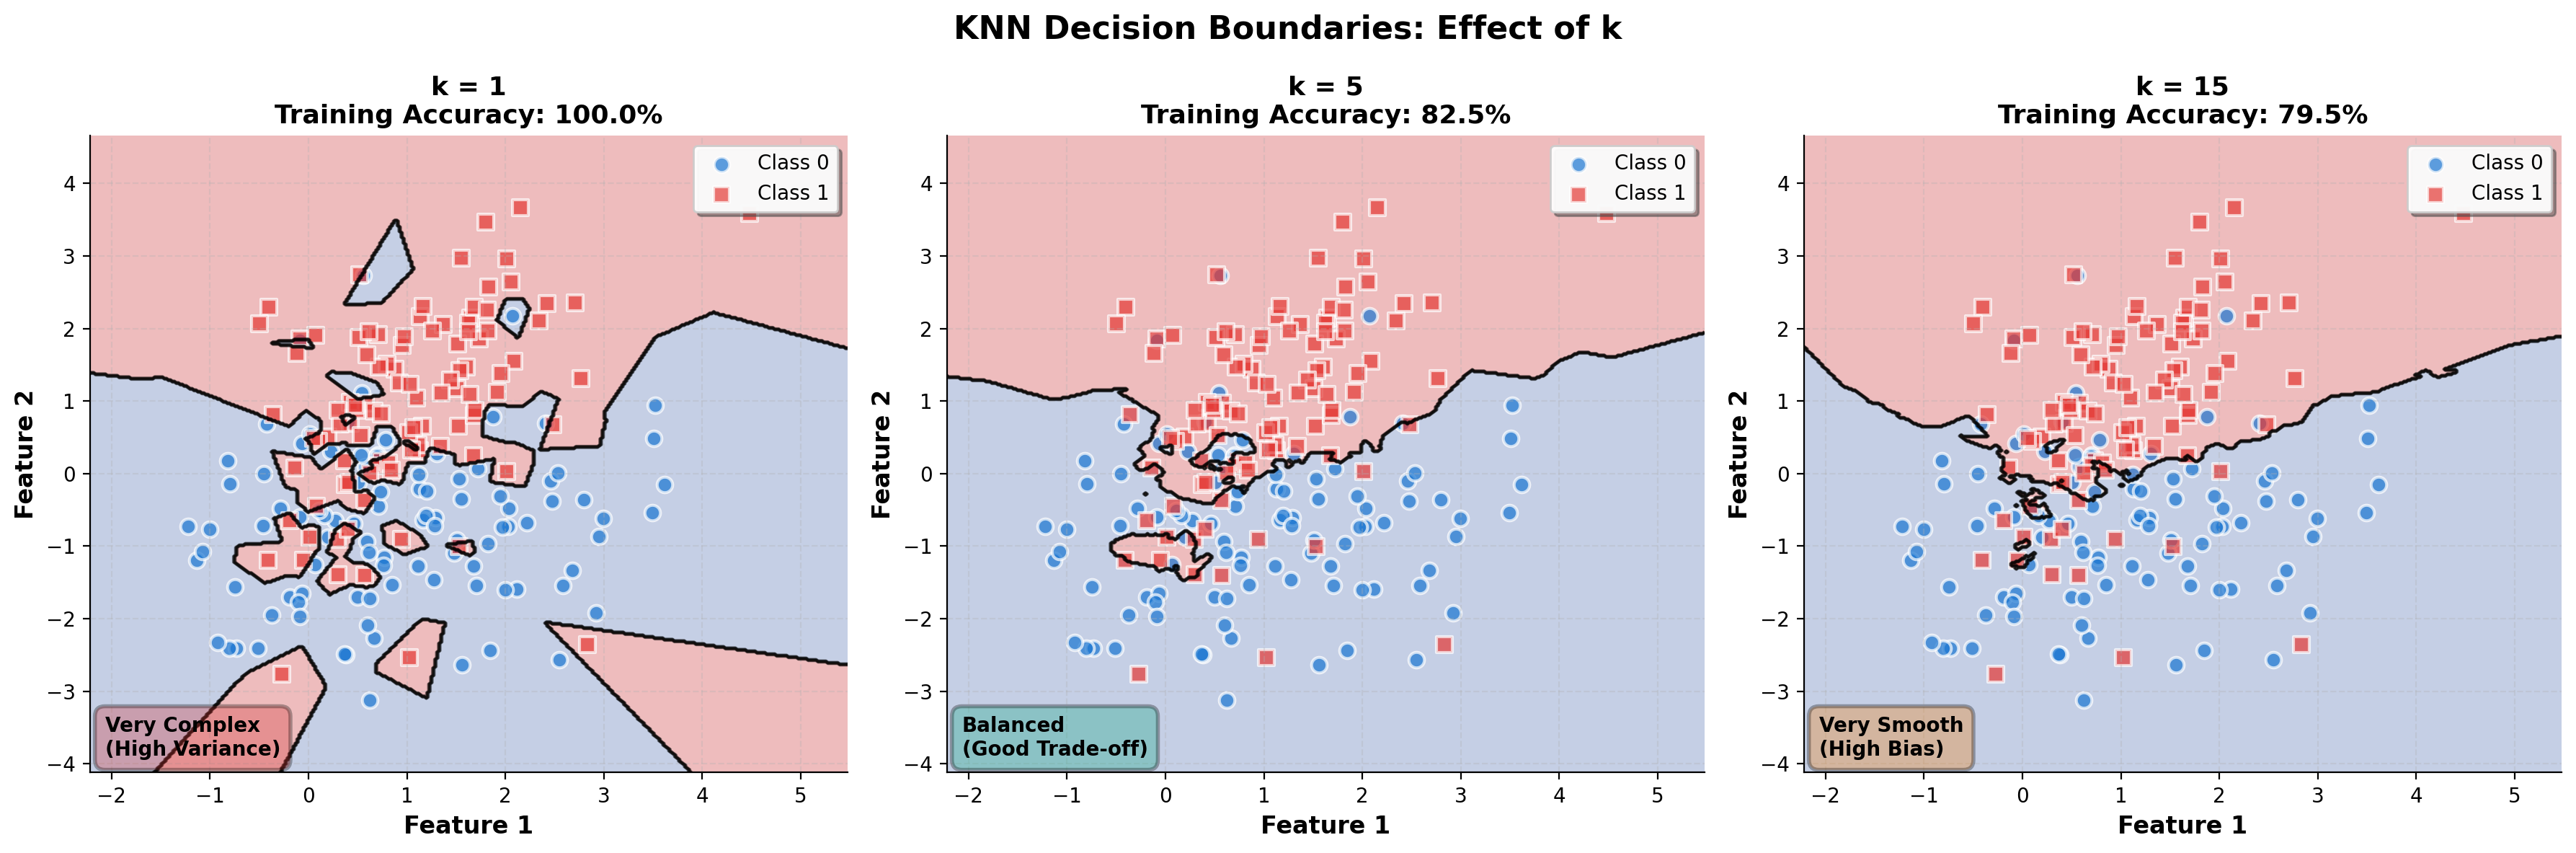
\includegraphics[width=\textwidth]{../figures/knn_decision_boundaries.png}

\begin{block}{\small Properties}
\begin{itemize}
\setlength{\itemsep}{0pt}
\small
\item Non-linear
\item Locally adaptive
\item No assumptions
\end{itemize}
\end{block}
\end{column}

\begin{column}{0.32\textwidth}
\centering
\textbf{Decision Tree}
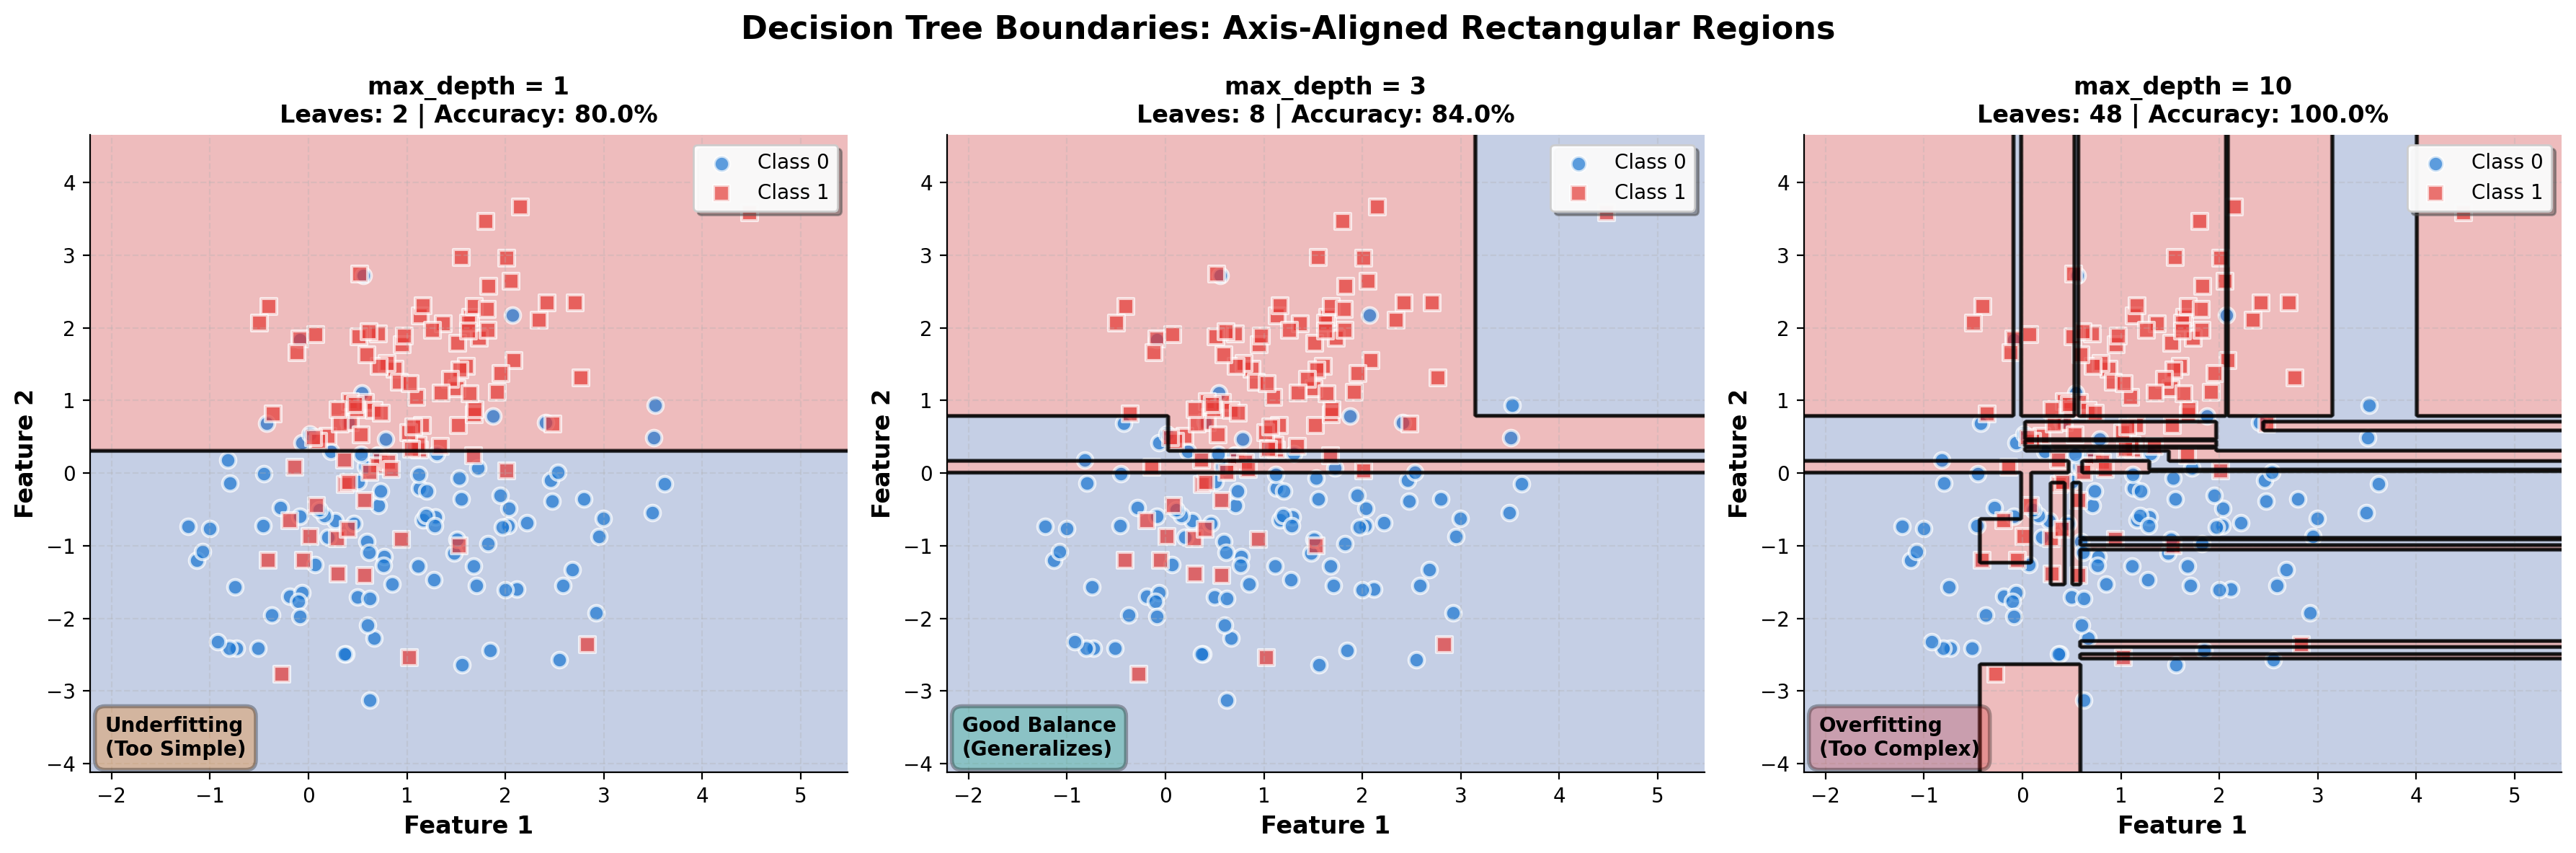
\includegraphics[width=\textwidth]{../figures/dt_decision_boundaries.png}

\begin{block}{\small Properties}
\begin{itemize}
\setlength{\itemsep}{0pt}
\small
\item Axis-aligned
\item Rectangular regions
\item Rule-based
\end{itemize}
\end{block}
\end{column}
\end{columns}

\vspace{0.15cm}

\begin{alertblock}{Key Insight}
Different methods create fundamentally different decision boundaries!
\end{alertblock}
\end{frame}

\begin{frame}{Detailed Comparison Table}

\small
\begin{table}
\centering
\begin{tabular}{p{2.5cm}p{3.5cm}p{3.5cm}p{3.5cm}}
\toprule
\textbf{Criterion} & \textbf{Naive Bayes} & \textbf{K-Nearest Neighbors} & \textbf{Decision Trees} \\
\midrule
\textbf{Type} & Probabilistic & Instance-based & Rule-based \\
\textbf{Training Time} & Very fast ($O(nd)$) & None ($O(1)$) & Medium ($O(nd\log n)$) \\
\textbf{Prediction Time} & Very fast ($O(Cd)$) & Slow ($O(nd)$) & Fast ($O(\log n)$) \\
\textbf{Memory} & Low (parameters only) & High (stores all data) & Medium (tree structure) \\
\textbf{Interpretability} & Medium (probabilistic) & Low (no model) & High (rules) \\
\textbf{Assumptions} & Feature independence & Locality principle & None \\
\textbf{Overfitting Risk} & Low & Medium-High & High (needs pruning) \\
\textbf{Handling Noise} & Robust & Sensitive & Medium \\
\textbf{Feature Scaling} & Not needed & Critical & Not needed \\
\textbf{Missing Values} & Can handle & Requires imputation & Can handle \\
\textbf{Categorical Features} & Natural & Needs encoding & Natural \\
\textbf{High Dimensions} & Good & Poor (curse) & Medium \\
\textbf{Imbalanced Data} & Prior adjustment & Class weighting & Sample weighting \\
\bottomrule
\end{tabular}
\end{table}

\vspace{0.1cm}

\begin{alertblock}{Recommendation}
Try all three methods and use cross-validation to choose the best for your data!
\end{alertblock}
\end{frame}

\begin{frame}{When to Use Each Method}

\begin{block}{Use Naive Bayes When:}
\begin{itemize}
\setlength{\itemsep}{2pt}
\item \textbf{Text classification} (spam filtering, document categorization)
\item \textbf{Real-time prediction} required (fast training and prediction)
\item \textbf{High-dimensional data} (works well even with many features)
\item \textbf{Small training set} (few parameters to estimate)
\item \textbf{Probabilistic output} needed (uncertainty estimates)
\item \textbf{Baseline model} (quick first approach)
\end{itemize}
\end{block}

\begin{block}{Use K-Nearest Neighbors When:}
\begin{itemize}
\setlength{\itemsep}{2pt}
\item \textbf{Small to medium dataset} ($n < 10,000$)
\item \textbf{Low dimensions} ($d < 20$)
\item \textbf{Non-linear patterns} present
\item \textbf{No training time} budget
\item \textbf{Anomaly detection} (outliers far from neighbors)
\item \textbf{Recommendation systems} (similarity-based)
\end{itemize}
\end{block}

\begin{block}{Use Decision Trees When:}
\begin{itemize}
\setlength{\itemsep}{2pt}
\item \textbf{Interpretability crucial} (medical, legal, financial decisions)
\item \textbf{Mixed feature types} (numerical and categorical)
\item \textbf{Feature interactions} important
\item \textbf{Non-linear relationships} expected
\item \textbf{Feature selection} needed (importance ranking)
\item \textbf{Building ensemble models} (Random Forest, XGBoost)
\end{itemize}
\end{block}
\end{frame}

\begin{frame}{Performance Comparison: Iris Dataset}

\begin{columns}[t]
\begin{column}{0.48\textwidth}
\begin{block}{Accuracy Comparison}
\begin{center}
\begin{tabular}{lcc}
\toprule
\textbf{Method} & \textbf{Train} & \textbf{Test} \\
\midrule
Naive Bayes & 96.0\% & 93.3\% \\
KNN ($k=5$) & 96.7\% & 96.7\% \\
Decision Tree (depth=3) & 98.3\% & 93.3\% \\
\bottomrule
\end{tabular}
\end{center}
\end{block}

\vspace{0.1cm}

\begin{block}{Timing Comparison}
\begin{center}
\begin{tabular}{lcc}
\toprule
\textbf{Method} & \textbf{Train} & \textbf{Predict} \\
\midrule
Naive Bayes & $<$1 ms & $<$1 ms \\
KNN & 0 ms & 2-5 ms \\
Decision Tree & 1-2 ms & $<$1 ms \\
\bottomrule
\end{tabular}
\end{center}
\end{block}
\end{column}

\begin{column}{0.48\textwidth}
\begin{exampleblock}{Key Insights}
\begin{itemize}
\setlength{\itemsep}{3pt}
\item All methods perform well on Iris
\item KNN best test accuracy
\item Decision tree shows slight overfit
\item Naive Bayes fastest overall
\item Timing differences negligible for small data
\end{itemize}
\end{exampleblock}

\vspace{0.1cm}

\begin{alertblock}{Important Note}
Performance varies greatly by dataset!

\vspace{0.05cm}

Always use cross-validation to compare methods on \textbf{your specific data}.
\end{alertblock}
\end{column}
\end{columns}
\end{frame}

% ========================================
% Section: Best Practices
% ========================================

\section{Best Practices \& Guidelines}

\begin{frame}{General Best Practices}

\begin{exampleblock}{Data Preprocessing}
\begin{itemize}
\setlength{\itemsep}{2pt}
\item \textbf{Handle missing values:} Impute or remove (method-dependent)
\item \textbf{Scale features:} Essential for KNN, not for Naive Bayes/Trees
\item \textbf{Encode categorical:} One-hot encoding (KNN), label encoding (Trees)
\item \textbf{Remove outliers:} Especially important for KNN
\item \textbf{Feature engineering:} Create domain-specific features
\item \textbf{Balance classes:} Use SMOTE, class weights, or resampling
\end{itemize}
\end{exampleblock}

\begin{exampleblock}{Model Selection \& Tuning}
\begin{itemize}
\setlength{\itemsep}{2pt}
\item \textbf{Split data properly:} Train/validation/test or cross-validation
\item \textbf{Tune hyperparameters:} Grid search or random search
\item \textbf{Compare multiple methods:} Don't commit to one prematurely
\item \textbf{Use appropriate metrics:} Accuracy, precision, recall, F1, AUC
\item \textbf{Validate generalization:} Check on held-out test set
\end{itemize}
\end{exampleblock}

\begin{exampleblock}{Model Interpretation}
\begin{itemize}
\setlength{\itemsep}{2pt}
\item \textbf{Analyze errors:} Confusion matrix, error analysis
\item \textbf{Feature importance:} Which features matter most?
\item \textbf{Decision boundaries:} Visualize for 2D data
\item \textbf{Cross-validate:} Report mean and std of metrics
\end{itemize}
\end{exampleblock}
\end{frame}

\begin{frame}{Common Pitfalls \& Solutions}

\begin{block}{Pitfall 1: Not Scaling Features (KNN)}
\textbf{Problem:} Features with large ranges dominate distance calculations

\textbf{Solution:} Always use StandardScaler or MinMaxScaler for KNN
\end{block}

\begin{block}{Pitfall 2: Using Test Data for Hyperparameter Tuning}
\textbf{Problem:} Test accuracy is optimistically biased

\textbf{Solution:} Use separate validation set or cross-validation
\end{block}

\begin{block}{Pitfall 3: Overfitting Deep Decision Trees}
\textbf{Problem:} Tree memorizes training data, poor generalization

\textbf{Solution:} Use pruning (max\_depth, min\_samples\_split, min\_samples\_leaf)
\end{block}

\begin{block}{Pitfall 4: Ignoring Class Imbalance}
\textbf{Problem:} Majority class dominates, poor minority class performance

\textbf{Solution:} Use class weights, SMOTE, or stratified sampling
\end{block}

\begin{block}{Pitfall 5: Naive Bayes with Correlated Features}
\textbf{Problem:} Independence assumption violated, overconfident predictions

\textbf{Solution:} Remove redundant features or use different method
\end{block}
\end{frame}

\begin{frame}{Hyperparameter Tuning Guide}

\begin{block}{Naive Bayes}
\begin{itemize}
\setlength{\itemsep}{2pt}
\item \textbf{Type:} Gaussian, Multinomial, or Bernoulli (match to data type)
\item \textbf{Smoothing $\alpha$:} Try [0.1, 0.5, 1.0, 2.0, 5.0] (for discrete features)
\item \textbf{Priors:} Uniform or class-balanced (adjust for imbalance)
\end{itemize}
\end{block}

\begin{block}{K-Nearest Neighbors}
\begin{itemize}
\setlength{\itemsep}{2pt}
\item \textbf{$k$:} Try odd values [1, 3, 5, 7, 9, 15, 21] (cross-validate!)
\item \textbf{Distance metric:} Euclidean, Manhattan, Minkowski
\item \textbf{Weights:} 'uniform' or 'distance' (weight by inverse distance)
\item \textbf{Algorithm:} 'brute', 'kd\_tree', 'ball\_tree' (for efficiency)
\end{itemize}
\end{block}

\begin{block}{Decision Trees}
\begin{itemize}
\setlength{\itemsep}{2pt}
\item \textbf{max\_depth:} Try [3, 5, 7, 10, 15, None] (most important!)
\item \textbf{min\_samples\_split:} Try [2, 10, 20, 50] (prevent overfitting)
\item \textbf{min\_samples\_leaf:} Try [1, 5, 10, 20] (smoother boundaries)
\item \textbf{criterion:} 'gini' or 'entropy' (usually similar performance)
\item \textbf{max\_features:} 'sqrt', 'log2', or None (for Random Forest)
\end{itemize}
\end{block}

\vspace{0.05cm}

\begin{alertblock}{Tip}
Use GridSearchCV or RandomizedSearchCV from scikit-learn for systematic tuning!
\end{alertblock}
\end{frame}

\begin{frame}{Feature Engineering Tips}

\begin{exampleblock}{For Naive Bayes}
\begin{itemize}
\setlength{\itemsep}{2pt}
\item \textbf{Text:} Use TF-IDF or count vectors (Multinomial NB)
\item \textbf{Discretize:} Bin continuous features if needed
\item \textbf{Remove correlated:} Drop highly redundant features
\item \textbf{Log transform:} For skewed distributions (Gaussian NB)
\end{itemize}
\end{exampleblock}

\begin{exampleblock}{For K-Nearest Neighbors}
\begin{itemize}
\setlength{\itemsep}{2pt}
\item \textbf{Dimensionality reduction:} Use PCA to reduce features
\item \textbf{Feature selection:} Remove irrelevant/noisy features
\item \textbf{Polynomial features:} Create interaction terms
\item \textbf{Distance metric:} Choose appropriate for domain (e.g., cosine for text)
\end{itemize}
\end{exampleblock}

\begin{exampleblock}{For Decision Trees}
\begin{itemize}
\setlength{\itemsep}{2pt}
\item \textbf{Keep raw features:} Trees handle non-linearity automatically
\item \textbf{Interaction terms:} Not needed (tree finds them)
\item \textbf{Categorical encoding:} Use label encoding (not one-hot)
\item \textbf{Create domain features:} Trees can use them directly
\end{itemize}
\end{exampleblock}

\vspace{0.05cm}

\begin{alertblock}{Universal Tip}
Domain knowledge is more valuable than complex feature engineering!
\end{alertblock}
\end{frame}

% ========================================
% Section: Summary
% ========================================

\section{Summary \& Conclusion}

\begin{frame}{Key Takeaways}

\begin{block}{Core Concepts}
\begin{itemize}
\setlength{\itemsep}{3pt}
\item \textbf{Classification:} Supervised learning for discrete labels
\item \textbf{Three fundamental approaches:} Probabilistic, instance-based, rule-based
\item \textbf{Different assumptions:} Match method to data characteristics
\item \textbf{Trade-offs:} Speed vs accuracy vs interpretability
\end{itemize}
\end{block}

\begin{block}{Method Summaries}
\begin{itemize}
\setlength{\itemsep}{3pt}
\item \textbf{Naive Bayes:} Fast probabilistic, assumes independence, great for text
\item \textbf{K-Nearest Neighbors:} Simple instance-based, non-parametric, slow prediction
\item \textbf{Decision Trees:} Interpretable rules, non-linear, prone to overfit
\end{itemize}
\end{block}

\begin{block}{Best Practices}
\begin{itemize}
\setlength{\itemsep}{3pt}
\item \textbf{Preprocess appropriately:} Scaling for KNN, encoding for trees
\item \textbf{Use cross-validation:} For model selection and hyperparameter tuning
\item \textbf{Try multiple methods:} No single best classifier for all problems
\item \textbf{Interpret results:} Understand why model makes predictions
\end{itemize}
\end{block}
\end{frame}

\begin{frame}{What We Covered}

\begin{enumerate}
\setlength{\itemsep}{4pt}
\item \textbf{Introduction:} Classification definition, applications, comparison with regression
\item \textbf{Naive Bayes:} Bayes theorem, independence assumption, Gaussian/Multinomial/Bernoulli variants, worked example
\item \textbf{K-Nearest Neighbors:} Distance metrics, algorithm, choosing $k$, curse of dimensionality, worked example
\item \textbf{Decision Trees:} CART algorithm, splitting criteria (Gini/Entropy), pruning, feature importance, worked example
\item \textbf{Comparison:} Decision boundaries, performance metrics, when to use each method
\item \textbf{Best Practices:} Data preprocessing, hyperparameter tuning, common pitfalls, feature engineering
\end{enumerate}

\vspace{0.2cm}

\begin{alertblock}{Next Steps}
\begin{itemize}
\setlength{\itemsep}{2pt}
\item \textbf{Practice:} Implement all three methods from scratch
\item \textbf{Experiment:} Try on different datasets (UCI ML Repository)
\item \textbf{Read ahead:} Ensemble methods (Random Forest, Boosting)
\item \textbf{Workshop:} Hands-on exercises in Jupyter notebook
\end{itemize}
\end{alertblock}
\end{frame}

\begin{frame}{Further Reading}

\begin{block}{Textbooks}
\begin{itemize}
\setlength{\itemsep}{3pt}
\item \textbf{Hastie et al.}: "The Elements of Statistical Learning" (Ch. 9: Additive Models, Trees)
\item \textbf{Bishop}: "Pattern Recognition and Machine Learning" (Ch. 4: Linear Models for Classification)
\item \textbf{Murphy}: "Machine Learning: A Probabilistic Perspective" (Ch. 3, 16: Generative and Discriminative Models)
\item \textbf{Mitchell}: "Machine Learning" (Ch. 3: Decision Tree Learning)
\end{itemize}
\end{block}

\begin{block}{Key Papers}
\begin{itemize}
\setlength{\itemsep}{3pt}
\item Breiman et al. (1984): "Classification and Regression Trees (CART)"
\item Quinlan (1986): "Induction of Decision Trees (ID3)"
\item Cover \& Hart (1967): "Nearest Neighbor Pattern Classification"
\item Rish (2001): "An Empirical Study of the Naive Bayes Classifier"
\end{itemize}
\end{block}

\begin{block}{Implementations}
\begin{itemize}
\setlength{\itemsep}{3pt}
\item \textbf{scikit-learn}: GaussianNB, MultinomialNB, KNeighborsClassifier, DecisionTreeClassifier
\item \textbf{Documentation}: https://scikit-learn.org/stable/supervised\_learning.html
\item \textbf{Tutorials}: scikit-learn user guide, Kaggle Learn
\end{itemize}
\end{block}
\end{frame}

\begin{frame}[standout]
\Huge Questions?

\vspace{1cm}

\large
Thank you for your attention!

\vspace{0.5cm}

\normalsize
Noel Jeffrey Pinton\\
Department of Computer Science\\
University of the Philippines - Cebu
\end{frame}

\end{document}
